%%%%%%%%%%%%%%%%%%%%%%%%%%%%%%%%%%%%%%%%%%%%%%%%%%%%%%%%%%%%
%%% LIVECOMS ARTICLE TEMPLATE FOR BEST PRACTICES GUIDE
%%% ADAPTED FROM ELIFE ARTICLE TEMPLATE (8/10/2017)
%%%%%%%%%%%%%%%%%%%%%%%%%%%%%%%%%%%%%%%%%%%%%%%%%%%%%%%%%%%%
%%% PREAMBLE
\documentclass[9pt,tutorial,pubversion]{livecoms}

\usepackage{lipsum} % Required to insert dummy text
\usepackage[version=4]{mhchem}
\usepackage{siunitx}
\usepackage{subcaption}
\usepackage{graphicx}
\usepackage{tabu}
\usepackage{color}
\usepackage{outlines}
\DeclareSIUnit\Molar{M}
\usepackage[italic]{mathastext}
%\usepackage{fixltx2e} % No longer necessary to load
\usepackage{listings}
\graphicspath{{figures/}}
\usepackage{verbatim} 

%%%%%%%%%%%%%%%%%%%%%%%%%%%%%%%%%%%%%%%%%%%%%%%%%%%%%%%%%%%%
%%% IMPORTANT USER CONFIGURATION
%%%%%%%%%%%%%%%%%%%%%%%%%%%%%%%%%%%%%%%%%%%%%%%%%%%%%%%%%%%%

\newcommand{\versionnumber}{2.0}  % you should update the minor version number in preprints and major version number of submissions.
\newcommand{\githubrepository}{\url{https://github.com/westpa/tutorials}}  %this should be the main github repository for this article

%%%%%%%%%%%%%%%%%%%%%%%%%%%%%%%%%%%%%%%%%%%%%%%%%%%%%%%%%%%%
%%% ARTICLE SETUP
%%%%%%%%%%%%%%%%%%%%%%%%%%%%%%%%%%%%%%%%%%%%%%%%%%%%%%%%%%%%
\title{A Suite of Tutorials for the WESTPA 2.0 Rare-Events Sampling Software
 [Article v\versionnumber]}

%\author[1*]{Firstname Middlename Surname}
%\author[1,2\authfn{1}\authfn{3}]{Firstname Middlename Familyname}
\author[1,\authfn{1}]{Anthony T. Bogetti}
\author[1,\authfn{1}]{Jeremy M. G. Leung}
\author[2,\authfn{1}]{John D. Russo}
\author[3,\authfn{1}]{She Zhang}
\author[3,\authfn{1}]{Jeff P. Thompson}
\author[4,\authfn{1}]{Ali S. Saglam}
\author[5,\authfn{1}]{Dhiman Ray}
\author[2]{Barmak Mostofian}
\author[1]{AJ Pratt}
\author[1]{Rhea C. Abraham}
\author[1]{Page O. Harrison}
\author[1]{Max Dudek}
\author[1]{Paul A. Torrillo}
\author[1]{Alex J. DeGrave}
\author[2]{Upendra Adhikari}
\author[4]{James R. Faeder}
\author[5]{Ioan Andricioaei}
\author[4]{Joshua L. Adelman}
\author[6]{Matthew C. Zwier}
\author[3]{David N. LeBard}
\author[2]{Daniel M. Zuckerman}
\author[1*]{Lillian T. Chong}

\affil[1]{Department of Chemistry, University of Pittsburgh, Pittsburgh, PA}
\affil[2]{Department of Biomedical Engineering, Oregon Health and Science University, Portland, OR}
\affil[3]{OpenEye Scientific, Santa Fe, NM}
\affil[4]{Department of Biological Sciences, University of Pittsburgh, Pittsburgh, PA}
\affil[5]{Department of Chemistry, University of California Irvine, Irvine, CA}
\affil[6]{Department of Chemistry, Drake University, Des Moines, IA}


\corr{ltchong@pitt.edu}{LTC}  % Correspondence emails.  FMS and FS are the appropriate authors initials.
%\corr{zuckermd@ohsu.edu}{DMZ}
\contrib[\authfn{1}]{These authors contributed equally to this work}

%OLD authors:  Not sure where the orcid's went? 
%MRS: Previous authors - the understanding is that the authors can change with versions.
%\author[1,\authfn{1}]{Anthony T. Bogetti}
%\author[1,\authfn{1}]{Jeremy M. G. Leung}
%\author[2,\authfn{1}]{John D. Russo}
%\author[3,\authfn{1}]{She Zhang}
%\author[3,\authfn{1}]{Jeff P. Thompson}
%\author[4,\authfn{1}]{Ali S. Saglam}
%\author[5,\authfn{1}]{Dhiman Ray}
%\author[1]{Rhea C. Abraham}
%\author[4]{James R. Faeder}
%\author[5]{Ioan Andricioaei}
%\author[4]{Joshua L. Adelman}
%\author[6]{Matthew C. Zwier}
%\author[3]{David N. LeBard}
%\author[2]{Daniel M. Zuckerman}
%\author[1*]{Lillian T. Chong}


%\orcid{Author 1 name}{AAAA-BBBB-CCCC-DDDD}
%\orcid{Author 2 name}{EEEE-FFFF-GGGG-HHHH}
\orcid{Anthony T. Bogetti}{0000-0003-0610-2879}
\orcid{Jeremy M. G. Leung}{0000-0001-7021-4619}
\orcid{John D. Russo}{0000-0002-2813-6554}
\orcid{She Zhang}{0000-0001-9265-4498}
\orcid{Jeff P. Thompson}{0000-0003-3134-9451}
\orcid{Ali S. Saglam}{0000-0002-6513-8401}
\orcid{Dhiman Ray}{0000-0002-7103-0886}
\orcid{Barmak Mostofian}{0000-0003-0568-9866}
\orcid{AJ Pratt}{0000-0002-5275-1020}
\orcid{Rhea C. Abraham}{0000-0003-3823-3822}
\orcid{Page O. Harrison}{0000-0003-2301-6016}
\orcid{Max Dudek}{0000-0001-8521-9543}
\orcid{Paul A. Torrillo}{0000-0002-4618-6061}
\orcid{Alex J. DeGrave}{0000-0001-9933-6273}
\orcid{Upendra Adhikari}{0000-0002-7568-1598}
\orcid{James R. Faeder}{0000-0001-8127-609X}
\orcid{Ioan Andricioaei}{0000-0002-6655-0721}
\orcid{Joshua L. Adelman}{0000-0001-9986-7533}
\orcid{Matthew C. Zwier}{0000-0002-0744-1146}
\orcid{David N. LeBard}{0000-0002-0979-800X}
\orcid{Daniel M. Zuckerman}{0000-0001-7662-2031}
\orcid{Lillian T. Chong}{0000-0002-0590-483X}



%\presentadd[\authfn{3}]{Department, Institute, Country}
%\presentadd[\authfn{4}]{Department, Institute, Country}

\blurb{This LiveCoMS document is maintained online on GitHub at \githubrepository; to provide feedback, suggestions, or help improve it, please visit the GitHub repository and participate via the issue tracker.}

%%%%%%%%%%%%%%%%%%%%%%%%%%%%%%%%%%%%%%%%%%%%%%%%%%%%%%%%%%%%
%%% PUBLICATION INFORMATION
%%% Fill out these parameters when available
%%% These are used when the "pubversion" option is invoked
%%%%%%%%%%%%%%%%%%%%%%%%%%%%%%%%%%%%%%%%%%%%%%%%%%%%%%%%%%%%
\pubDOI{10.33011/livecoms.5.1.1655}
\pubvolume{5}
\pubissue{1}
\pubyear{2023}
\articlenum{1655}
\datereceived{18 May 2022}
\dateaccepted{14 January 2023}


\newcommand{\hl}[1]{{\colorbox{orange}{#1}}}


%%%%%%%%%%%%%%%%%%%%%%%%%%%%%%%%%%%%%%%%%%%%%%%%%%%%%%%%%%%%
%%% ARTICLE START
%%%%%%%%%%%%%%%%%%%%%%%%%%%%%%%%%%%%%%%%%%%%%%%%%%%%%%%%%%%%

\begin{document}

\begin{frontmatter}
\maketitle

\begin{abstract}
%OLD:
The weighted ensemble (WE) strategy has been demonstrated to be highly efficient in generating pathways and rate constants for rare events such as protein folding and protein binding using atomistic molecular dynamics simulations. 
Here we present two sets of tutorials instructing users in the best practices for preparing, carrying out, and analyzing WE simulations for various applications using the WESTPA software. 
%Users are expected to already have significant experience with running standard molecular dynamics simulations using the underlying dynamics engine of interest (e.g. Amber, Gromacs, OpenMM). 
The first set of more basic tutorials describes a range of simulation types, from a molecular association process in explicit solvent to more complex processes such as host-guest association, peptide conformational sampling, and protein folding. 
%
%NEW: 
The second set ecompasses six advanced tutorials instructing users in the best practices of using key new features and plugins/extensions of the WESTPA 2.0 software package, which consists of major upgrades for larger systems and/or slower processes. 
The advanced tutorials demonstrate the use of the following key features: (i) a generalized resampler module for the creation of “binless” schemes, (ii) a minimal adaptive binning scheme for more efficient surmounting of free energy barriers, (iii) streamlined handling of large simulation datasets using an HDF5 framework, (iv) two different schemes for more efficient rate-constant estimation, (v) a Python API for simplified analysis of WE simulations, and (vi) plugins/extensions for Markovian Weighted Ensemble Milestoning and WE rule-based modeling for systems biology models.
Applications of the advanced tutorials include atomistic and non-spatial models, and consist of complex processes such as protein folding and the membrane permeability of a drug-like molecule. 
Users are expected to already have significant experience with running conventional molecular dynamics or systems biology simulations.% and completed the previous suite of WESTPA tutorials. 
\end{abstract}

\end{frontmatter}

\tableofcontents


%\vspace{0.5cm}
%\hl{Lillian - check author list}\\
%\hl{Github repo must be modified - see main.tex comment}%link given must at least point to second repo of original tutorials.  MR Shirts: ``One suggestion is for there to be three repositories – Westpa1 tutorials, Westpa2 tutorials, and the paper.   Then the paper repository can then point to as many other repositories for the actual tutorials as desired. It makes it slightly less direct, but allows for arbitrary organization of the tutorials.''}

\section{Introduction and Scope of Tutorials}

The WESTPA (Weighted Ensemble Simulation Toolkit with Parallelization and Analysis) software package is a highly scalable implementation of the weighted ensemble (WE) path sampling strategy \citep{huber_weighted-ensemble_1996,zuckerman_weighted_2017} that has helped transform what is feasible for molecular simulations in the generation of pathways for long-timescale processes (> µs) with rigorous kinetics.
Among these simulations are atomically detailed simulations of protein folding \citep{adhikari_computational_2019}, protein-protein binding \citep{saglam_proteinprotein_2019}, protein-ligand unbinding \citep{lotz_unbiased_2018}, and the large-scale opening of the SARS-CoV-2 spike protein \citep{sztain_glycan_2021}. 
The latter involved the slowest process (seconds-timescale) yet studied for a massive system (one million atoms) using WE simulations. 
As a “bleeding edge” application, these efforts have motivated major upgrades to WESTPA (version 2.0) that enable the sampling of processes at even longer timescales and more streamlined handling of large datasets \citep{russo_westpa_2022}. 
Like its predecessor, WESTPA 2.0 is a Python package that is (i) interoperable, enabling the use of any type of stochastic dynamics simulation (e.g., MD or Monte Carlo simulations) and any model resolution (e.g., atomistic, coarse-grained, non-spatial or spatially resolved systems biology models) \citep{donovan_efficient_2013,donovan_unbiased_2016}; and (ii) extensible, making it straightforward to modify existing modules or create plug-ins in order to support new scientific efforts. 

Here, we present a suite of six advanced tutorials for applying major upgrades in the WESTPA 2.0 software package. 
For general prerequisites to attempting these tutorials, please see \textbf{Section 1.2} below. 
Among these tutorials is one involving the Markovian Weighted Ensemble Milestoning (M-WEM) approach \citep{Ray2022Markovian}, which interfaces the WE strategy with another path sampling method called milestoning \citep{Faradjian2004Computing,West2007Extending}. 
In the final tutorial, we broaden the scope of path sampling to a systems biology application involving a WESTPA plugin for enhancing the efficiency of Monte Carlo simulations using the BioNetGen systems biology package \citep{harris_bionetgen_2016, tapia_mcell-r_2019}. 
All files for the tutorials can be found online in the WESTPA 2.0 Tutorials GitHub repository {\url{https://github.com/westpa/westpa2_tutorials}}. 
In each tutorial, we outline learning objectives and expected outcomes. 

After completing \textbf{Advanced Tutorial 3.1}, which involves the simulation of Na\textsuperscript{+}/Cl\textsuperscript{-} association, the user should be able to:
\begin{enumerate}
  \item Create a customized binless resampler scheme for splitting and merging trajectories based on by k-means clustering using the \verb|BinlessMapper| resampler module;
  \item Initiate a WE simulation from multiple starting conformations;
  \item Combine multiple WE simulations for analysis using the \verb|w_multi_west| multitool;
  \item Perform post-simulation analysis using the \verb|w_crawl| tool.
\end{enumerate}

After completing \textbf{Advanced Tutorial 3.2} involving the simulation of drug membrane permeation, the user should be able to:
\begin{enumerate}
  \item Set up a double membrane bilayer system for permeability studies; 
  \item Use the highly scalable HDF5 framework for more efficient restarting, storage, and analysis of simulations;
  \item Apply the minimal adaptive binning (MAB) scheme.
\end{enumerate}

After completing \textbf{Advanced Tutorial 3.3} involving the simulation of ms-timescale protein folding, the user should be able to:
\begin{enumerate}
  \item Apply the haMSM plugin for periodic reweighting of simulations;
  \item Use the \verb|msm_we| package to build an haMSM from WE data;
  \item Estimate the distribution of first passage times.
\end{enumerate}

After completing \textbf{Advanced Tutorial 3.4} involving the creation of custom analysis routines and calculation of rate constants, the user should be able to:
\begin{enumerate}
  \item Access simulation data in a \verb|west.h5| file using the high-level \verb|Run| interface of the \verb|westpa.analysis| Python API and retrieve trajectory data using the \verb|BasicMDTrajectory| and \verb|HDF5MDTrajectory| readers;
  \item Access steady-state populations and fluxes from the \verb|assign.h5| and \verb|direct.h5| data files, convert fluxes to rate constants, and plot the rate constants using an appropriate averaging scheme;
  \item Apply the RED analysis scheme to estimate rate constants from shorter trajectories;
\end{enumerate}

After completing \textbf{Advanced Tutorial 3.5} involving simulations of alanine dipeptide using the M-WEM method, the user should be able to:
\begin{enumerate}
  \item Install the M-WEM software and perform a M-WEM simulation;
  \item Create milestones to define the M-WEM progress coordinate;
  \item Analyze an M-WEM simulation to compute the mean first passage time, committor, and free energy landscape.
\end{enumerate}

After completing \textbf{Advanced Tutorial 3.6} involving rule-based modeling of a gene switch motif using the WESTPA/BNG plugin, the user should be able to:
\begin{enumerate}
  \item Install the WESTPA/BNG plugin and set up a WESTPA/BNG simulation; 
  \item Apply adaptive Voronoi binning, which can be used for both non-spatial and molecular systems; 
  \item Run basic analyses tailored for high-dimensional WESTPA simulations. 
\end{enumerate}

In each tutorial, all of the required software, including the dynamics engine and analysis tools, are freely available with easily-accessible online documentation.
Please note the version of each software package listed in the \textbf{Computational Requirements} section of each tutorial. 

% for single column figure don't include the *
\begin{figure*}[ht]
\centering
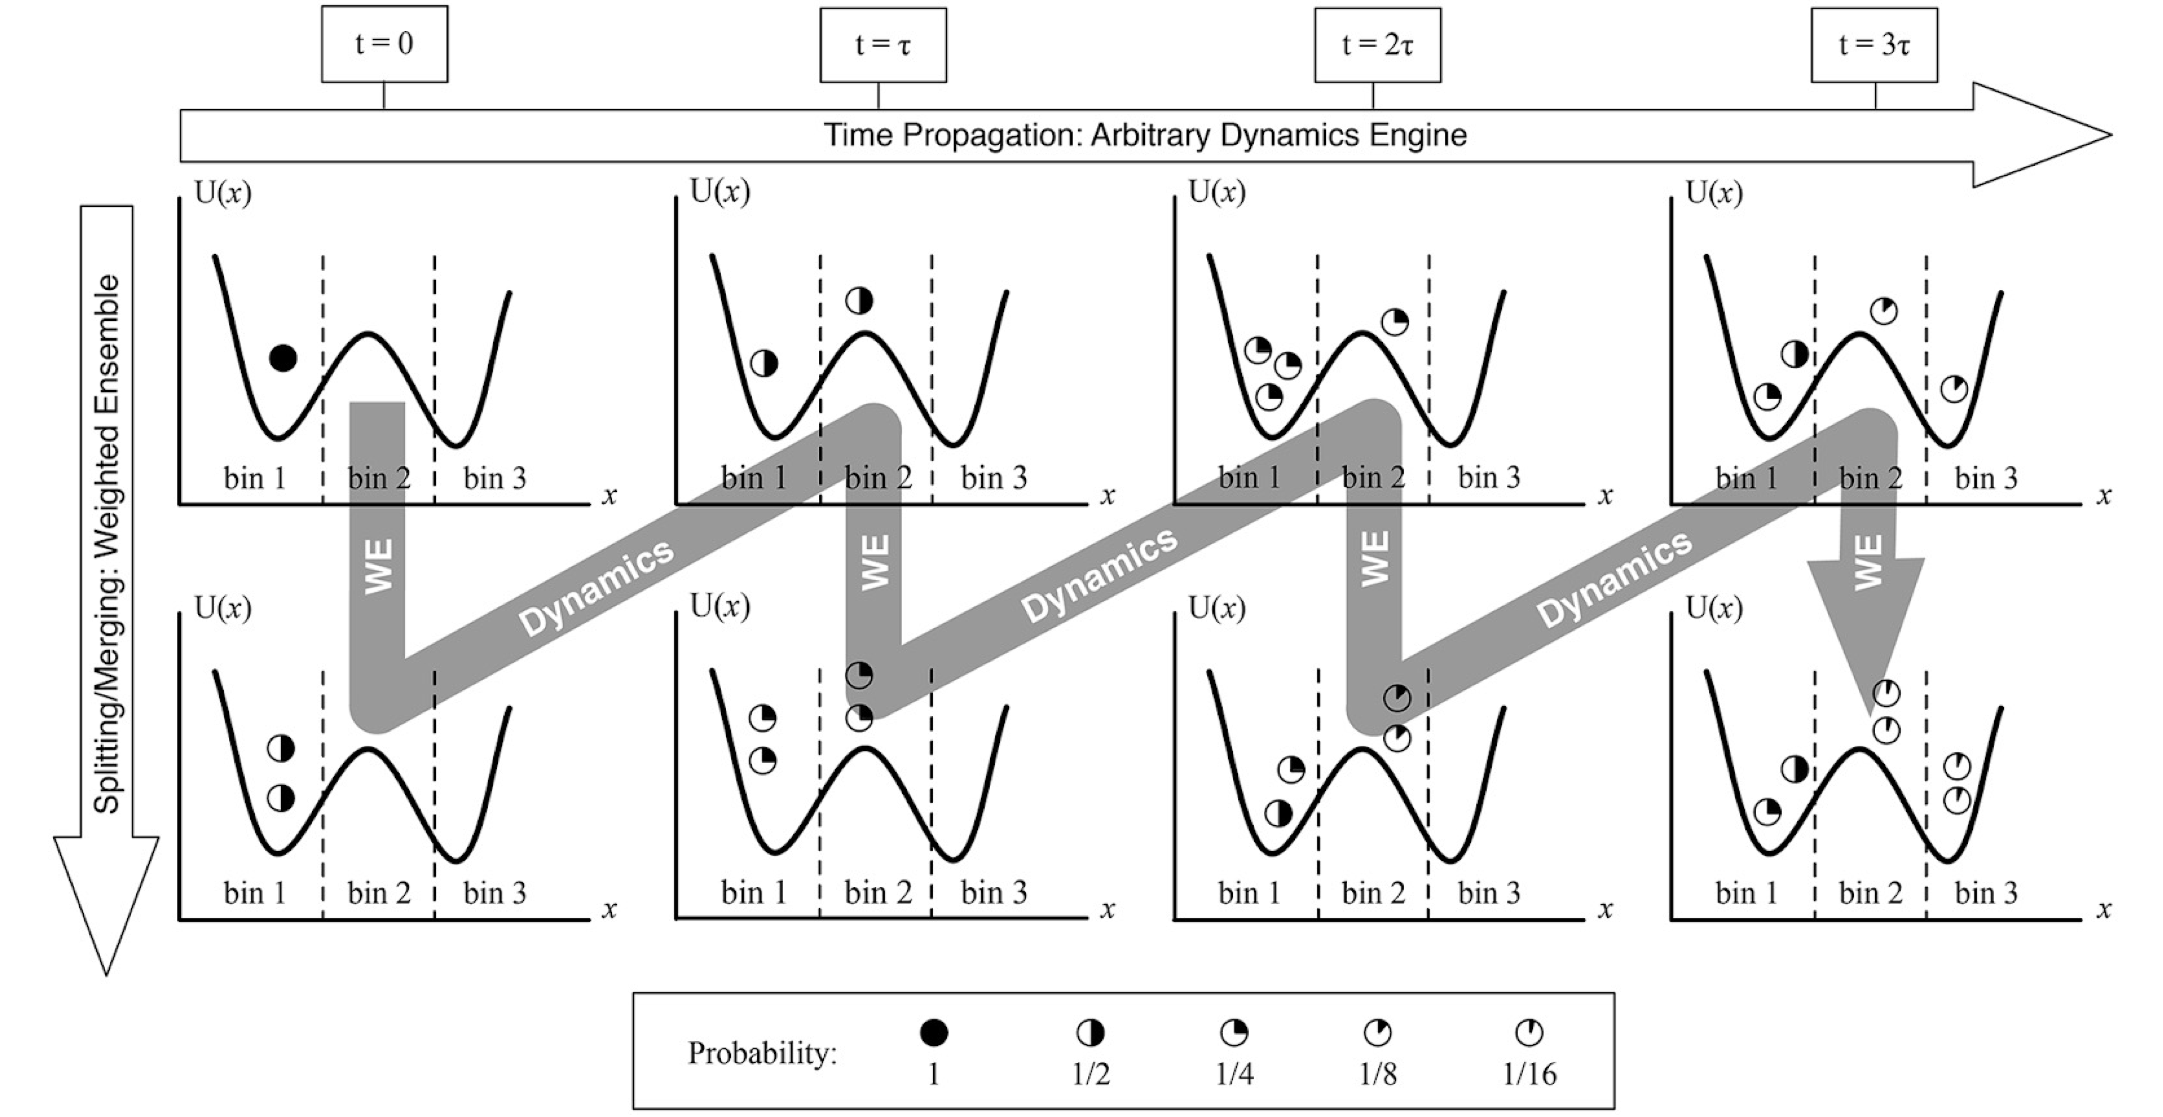
\includegraphics[width=\linewidth]{figure1_WE}
\caption{Overview of the weighted ensemble (WE) strategy \citep{donovan_unbiased_2016}.  WE typically employs bins, demarcated here by dashed vertical lines, to guide a set of trajectories to sample throughout configuration space.
Using only ordinary dynamics---without biasing forces---WE replicates (“splits”) trajectories in unoccupied or under-occupied regions of space and prunes (“merges”) trajectories in over-occupied regions, according to the user-specified allocation scheme which here is a target of two trajectories per bin.
Throughout the process, weights (partially filled circles) are tracked by statistical rules of inheritance that ensure that the overall ensemble dynamics are consistent with non-equilibrium statistical mechanics \citep{zhang_exact_2010}.
Figure adapted with permission from \citep{donovan_efficient_2013}.}
\end{figure*}

\subsection{The Weighted Ensemble Strategy}

WE is a highly-parallel path sampling strategy for generating rare events, for studying non-equilibrium steady states, and less commonly, for studying equilibrium properties. 
At heart, it is a simple and flexible strategy which is agnostic to system type and which therefore lends itself to numerous applications and optimizations. 
The properties of WE, including strengths and limitations, have been reviewed in detail before \citep{zuckerman_weighted_2017}, although improvements continue to be developed \citep{donyapour_revo_2019, copperman_accelerated_2020, torrillo_minimal_2021, degrave_red_2021, aristoff_optimizing_2020}. 
Here, we briefly review key aspects of WE.

\textbf{The Basic WE Procedure.} See \textbf{Figure 1}. 
WE orchestrates multiple trajectories---each assigned a weight---run in parallel by stopping them at regular time intervals of length $\tau$ (typically a large multiple of the underlying simulation time step), examining the trajectories, and restarting a new set of trajectories. 
The new trajectories are always continuations of the existing set, but some trajectories may not be continued (they are “pruned”) and others may be replicated. 
Discontinued trajectories result from probabilistic “merge” events where a continued trajectory absorbs the weight of one that is pruned. 
Replicated trajectories are said to be “split” with the original weight shared equally among the copies. 
Usually bins in configuration space are used to guide split and merge events based on a target number of trajectories for each bin, but any protocol---including binless strategies highlighted below---may be used for this purpose.
Regardless of the resampling protocol, a “recycling” protocol often is used whereby events reaching a user-specified target state are re-initiated according to a specified distribution of start states \citep{bhatt_steady-state_2010}.
This recycling protocol focuses all sampling on a single direction of a process of interest and has valuable properties as noted below.

\textbf{WE is Resampling, and Hence Unbiased.} The simple steps defining WE simulations stem from its basis as a statistical “resampling” procedure \citep{zhang_exact_2010}. 
The split/merge steps generate a statistically equivalent (re)sample of an initial trajectory set by increasing/reducing trajectory density in some regions of configuration space at a given time, using weight adjustments to maintain the underlying trajectory distribution. 
The trajectory set is therefore unbiased at all times, i.e., average time-dependent observables derived from many WE runs will match the average of a large number of conventional simulations without splitting or merging events \citep{zhang_exact_2010}. 
Furthermore, the distributions of transition path times (“barrier crossing times”) from WE runs match those from converged conventional simulations, and can be generated in orders of magnitude less computing time \citep{zwier_efficient_2011, zheng_simulating_2007}. 
The lack of bias in the dynamics of WE runs holds true regardless of whether recycling is employed.

\textbf{Observables and Ensembles Sampled by WE.} WE can yield transient and/or steady-state observables. 
When recycling is not used, WE provides pathways, i.e., sequences of conformations in a transition and the frequencies of those sequences, in addition to time-dependent observables as the system relaxes to equilibrium, e.g., the probability of a given event at a given time after initiation in the chosen starting state.
Complex systems are unlikely to relax fully to equilibrium during a WE simulation. 
With a recycling protocol, the system will not relax to equilibrium but instead to a non-equilibrium steady state (NESS) that has steady probability flow from initial to target state. 
If reached, the NESS provides a simple mechanism for computing rate constants via the Hill relation \citep{bhatt_steady-state_2010}. 
However, although relaxation to a NESS can be considerably faster than relaxation to equilibrium \citep{copperman_transient_2019,zuckerman_discrete-state_nodate}, the process may be too slow for WE to reach NESS on practical timescales, motivating the haMSM approach \citep{adhikari_computational_2019,copperman_accelerated_2020} described below.

\textbf{Resampling Introduces Correlations, which Increase Variance.} WE has intrinsic limitations, like any method \citep{chong_path-sampling_2017}, and it is essential to understand them. 
Most fundamentally, splitting and merging introduce correlations into the sampled trajectory ensemble that could decrease its information content. 
These stem primarily from splitting events: multiple trajectories share an identical history up to the time of the split event and hence do not contribute fully independent information to any observable.
These correlations, in turn, can lead to large run-to-run variance \citep{adhikari_computational_2019} because the trajectory ensemble in each WE run results from a relatively small number of “parent” trajectories which have been split repeatedly.
This variance is addressed to some extent by the iterative haMSM protocol described below, and more directly by ongoing mathematical optimizations noted below.  
Importantly, correlations within WE ensembles lead to significant challenges in quantifying uncertainty \citep{zuckerman_weighted_2017,mostofian_statistical_2019}.

\textbf{Ongiong Efforts at Optimization and Variance Reduction.} Because WE is unbiased so long as a correct resampling protocol is used \citep{zhang_exact_2010}, there is an opportunity to reduce the run-to-run variance noted above by improved resampling procedures. 
In the context of binned WE simulations, both the construction of bins and the number of trajectories per bin can be optimized based on a recently developed mathematical formulation \citep{aristoff_analysis_2018, aristoff_optimizing_2020} or based on heuristics \citep{torrillo_minimal_2021}. 
Bins do not need to be kept static over time \citep{zhang_exact_2010,dickson_wexplore_2014,torrillo_minimal_2021}. 
Optimization approaches are actively being studied and incorporated into WESTPA as appropriate.

\textbf{WE Cannot Solve Every Problem.} Despite its great strengths and highly notable achievements \citep{lotz_unbiased_2018, sztain_glycan_2021, adhikari_computational_2019}, users should not assume WE can tackle any problem.
Independent of the correlation/variance issues noted above, certain systems will remain too complex for WE given current hardware and algorithms.
In every system, there is a minimum transition path time t\textsubscript{TP} (also called t\textsubscript{b}) \citep{zuckerman_transition_2002, zhang_efficient_2007} for physically realistic events which sets an absolute requirement on sampling required: in a WE run, a set of trajectories exceeding the minimum t\textsubscript{TP} must be generated, which may be a prohibitive cost.
Additionally, even if the necessary computing resources are available, current binning and resampling strategies might not be sufficient to generate events of interest. 
And finally, even if events of interest are generated, the sampled trajectories may be insufficient for producing observables of interest such as a reliable estimate of the rate constant.

\subsection{Prerequisites}

\textbf{Background Knowledge and Experience.} All tutorials here are at the advanced level. 
Thus, a prerequisite for these tutorials is completion of the Basic and Intermediate WESTPA tutorials \citep{bogetti_suite_2019}, which have been updated for use with WESTPA version 2.0 ({\url{https://github.com/westpa/westpa_tutorials}}). 
Users should already have extensive experience running conventional simulations using the underlying dynamics engine of interest (Amber \citep{case_amber_2022}, OpenMM \citep{eastman_openmm_2017}, BioNetGen \citep{harris_bionetgen_2016}, etc.). 
Prior to applying the WE strategy to their own systems, we suggest that users run multiple conventional simulations to (i) ensure that the preparation of the system and propagation of dynamics is according to best practices (e.g., see \citep{braun_best_2019}), (ii) identify potential progress coordinates and initially define the target state, and (iii) estimate the ns/day on a single CPU/GPU for your system and storage needs for the full-scale WE simulation. 
We highly recommend that new WESTPA users read this review article \citep{zuckerman_weighted_2017} and this introduction to non-equilibrium physics of trajectories \citep{zuckerman_gentle_2021}. 

\textbf{Software Requirements.} The WESTPA 2.0 software is a standard Python package that can be used on any Unix operating system. 
The software requires Python versions $\geq$3.7 and a number of standard Python scientific computing packages. 
We recommend installing WESTPA either as a PyPI or conda package using miniconda. 
Both packages provide all required software dependencies and can be installed using one-line commands: (1) \verb|python -m pip install westpa| or (2) \verb|conda install -c conda-forge westpa|. 
Note that it is a best practice to install WESTPA into an isolated virtual or conda environment, along with the dependencies specific to your project. 
Due to the use of the MDTraj Python library with the WESTPA 2.0 HDF5 framework, certain modifications to the installation procedure are required for running WESTPA 2.0 on ppc64Ie architectures (e.g., TACC Longhorn or ORNL Summit supercomputers; see {\url{https://github.com/westpa/westpa/wiki/Alternate-Installation-Instructions}}). 

WESTPA 2.0 is designed to be interoperable with any dynamics engine, requiring an external dynamics engine to propagate the dynamics in a WE simulation.
Please see the prerequisite sections of each tutorial for additional software requirements that are specific to that tutorial.

\textbf{Hardware Requirements.} Like its predecessor, WESTPA 2.0 is highly-scalable on CPUs/GPUs, making optimal use of high-performance computing (HPC) clusters available at academic institutions or supercomputing centers. 
Memory requirements are dependent on the underlying dynamics engine, e.g., \textasciitilde1 GB per CPU core (or GPU) for atomistic MD simulations. 
Users should refer to the best practices of their dynamics engine of choice to determine the optimal allocation of resources for each CPU/GPU. 
The most efficient way to run WESTPA is to use a computing resource that provides the user with a number of CPUs/GPUs---all the same processor speed---that either matches the number of trajectories per WE iteration or a number by which the number of trajectories at any point in time is evenly divisible. 
WE can nevertheless run on heterogeneous hardware (different processor or memory bus speeds) or with trajectory counts that do not divide evenly onto CPUs/GPUs, but this scenario decreases efficiency as some processors are inevitably idle for at least a portion of the overall runtime.

Users can estimate the approximate storage space required for their project by taking the product of the following: (i) amount of disk space required for storing data from one trajectory segment of length $\tau$, (ii) the maximum number of trajectories per WE iteration, and (iii) the total number of WE iterations required to generate a reasonable maximum trajectory length. 
To optimize the use of storage space, we recommend that users tar up trajectory files into a single file for each WE iteration and remove coordinates of the system that are not of primary interest (e.g., solvent coordinates for certain processes). 
We note that the WESTPA 2.0 HDF5 framework dramatically reduces the storage space required for trajectory coordinates by consolidating the data from millions of small trajectory files into a relatively small number of larger HDF5 files, reducing the large overhead from the file system that results from the storage of numerous small trajectory files. 
By doing so, the HDF5 framework also alleviates potential I/O bottlenecks when a large amount of simulation files are written after each WE iteration. 

\section{Recommended Simulation Workflow with WESTPA 2.0 Upgrades}

Given the major upgrades in the WESTPA 2.0 software package \citep{russo_westpa_2022}, we recommend the three-stage simulation workflow illustrated in \textbf{Figure 2}. Details of the particular schemes are provided in the tutorials.

% for single column figure don't include the *
\begin{figure}[ht]
\centering
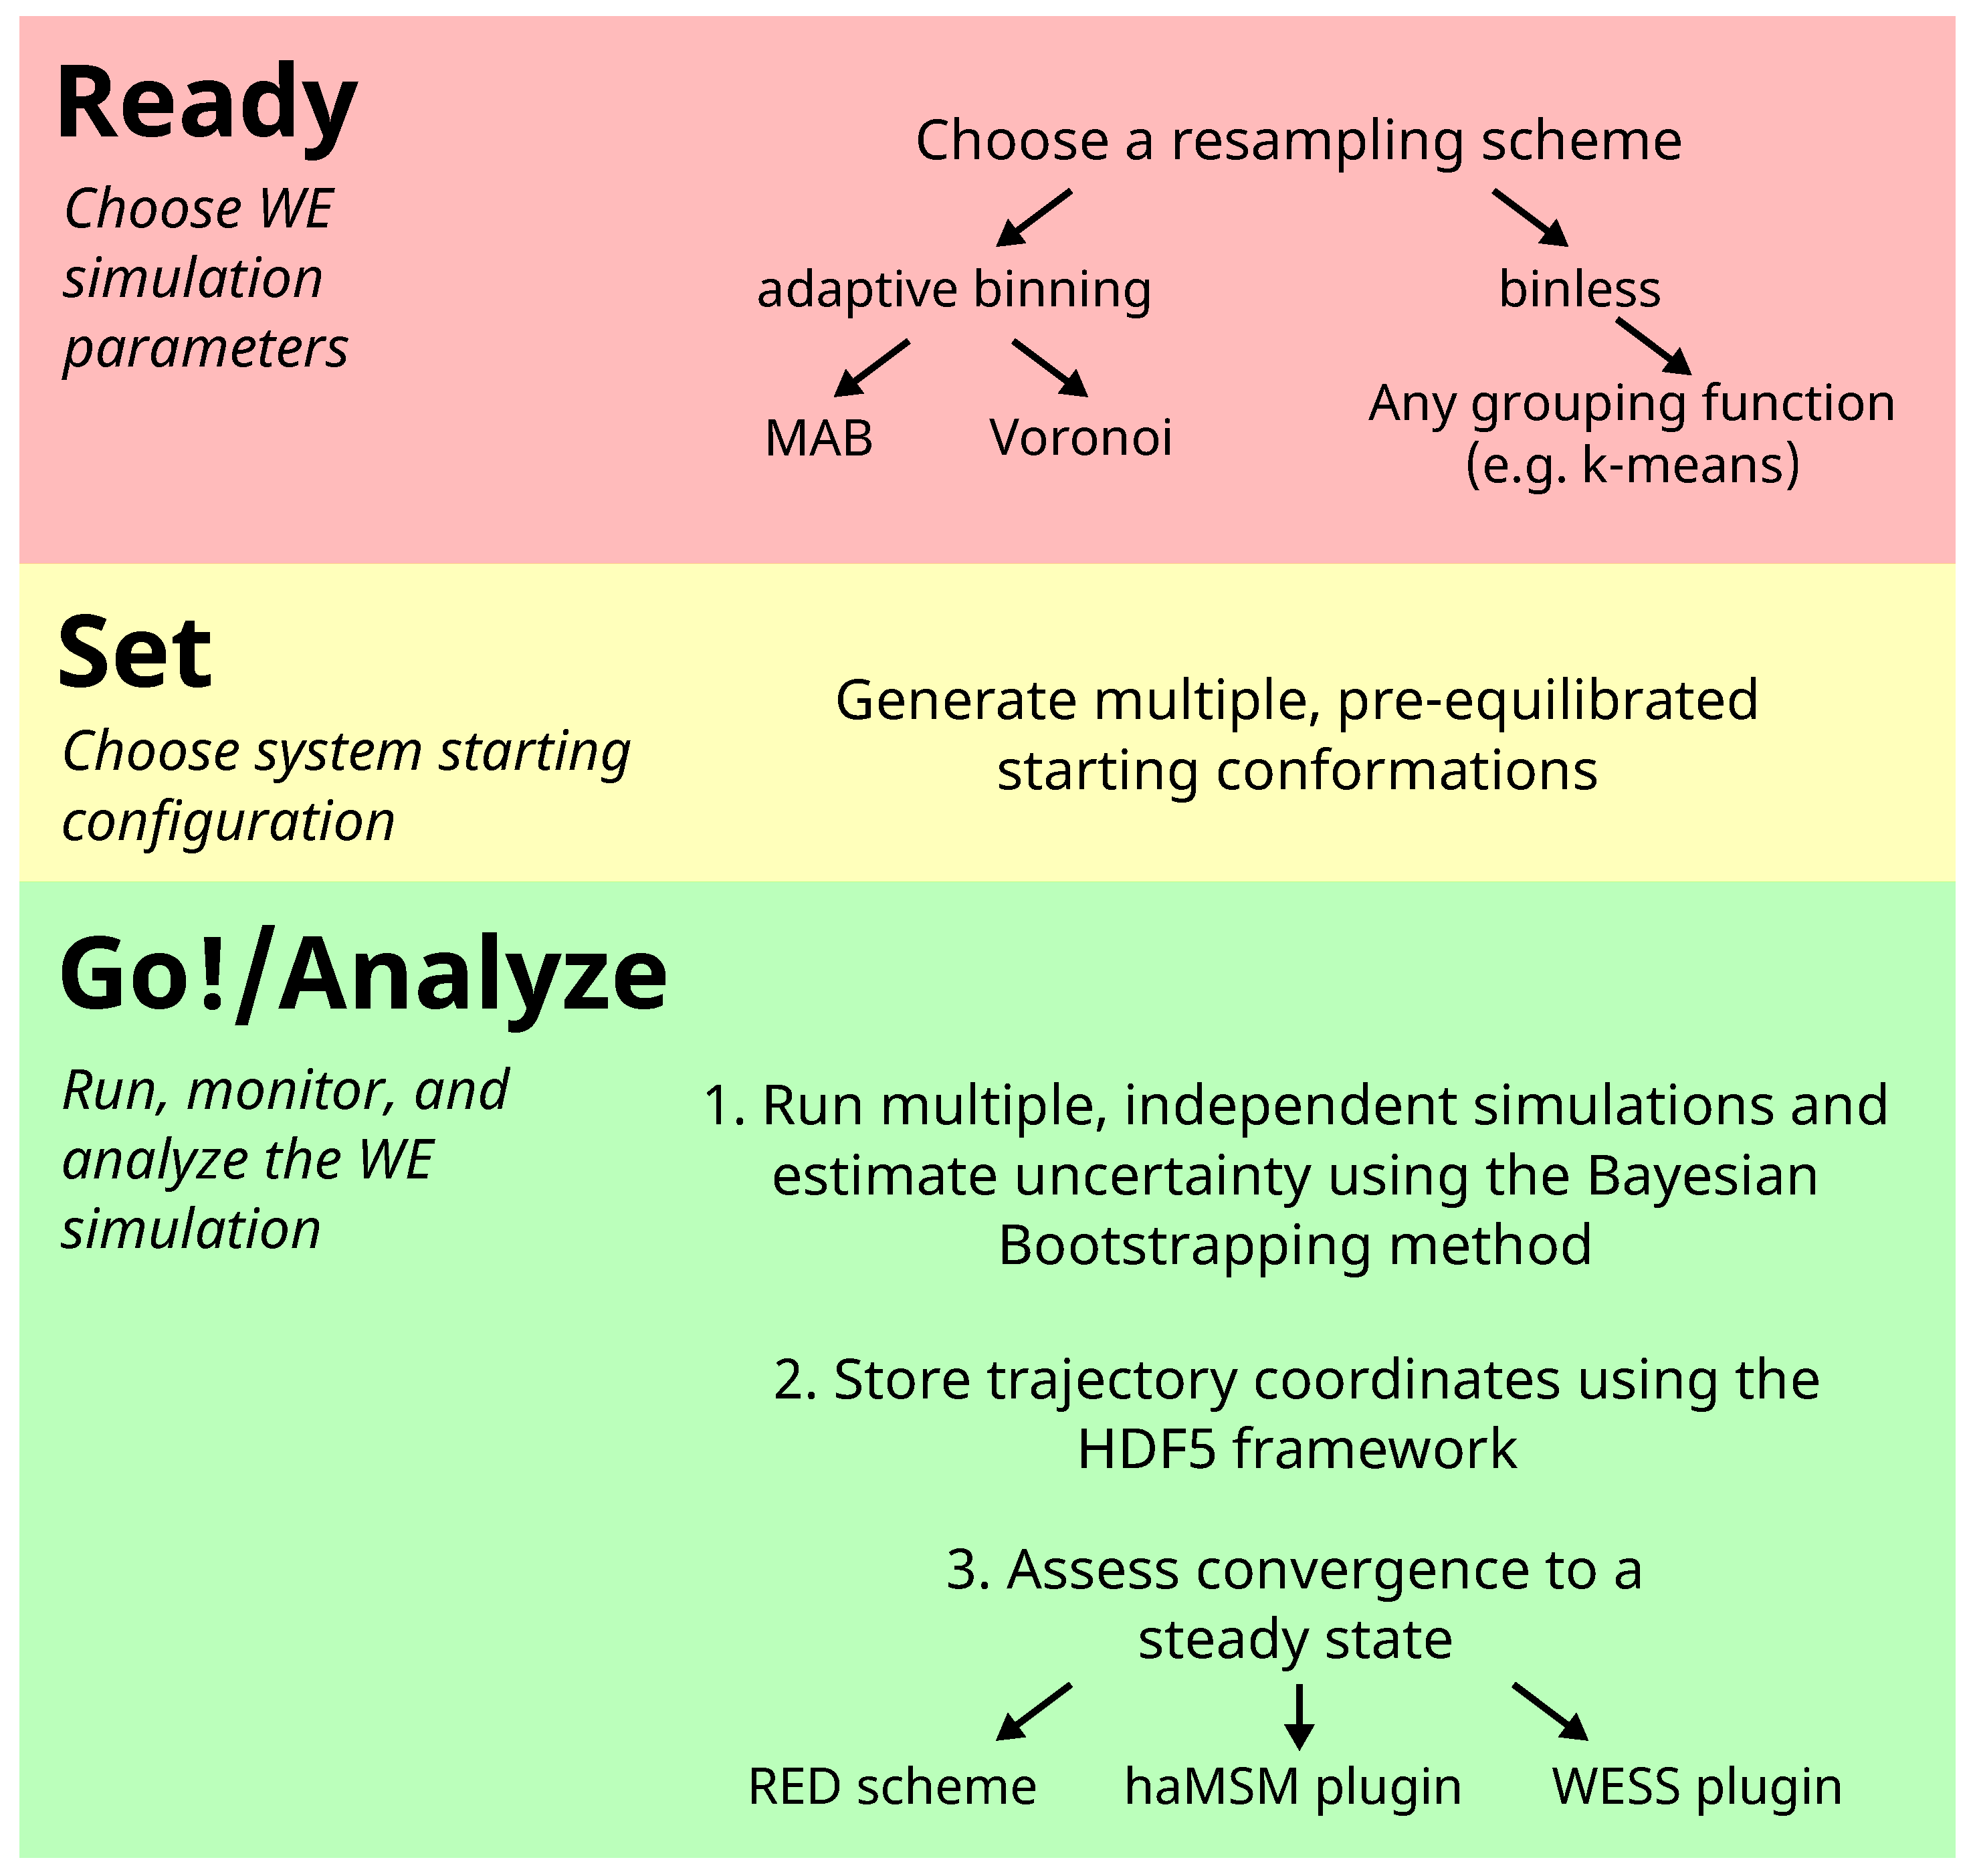
\includegraphics[width=\columnwidth]{figures/Figure2_workflow.pdf}
\caption{Recommended simulation workflow that makes use of major upgrades in the WESTPA 2.0 software.}
\end{figure}

In the first (“Ready”) stage, if one uses a binned resampling scheme, we recommend using one of the two adaptive binning schemes available in WESTPA 2.0: the minimal adaptive binning (MAB) scheme or adaptive Voronoi binning scheme.
These adaptive binning schemes enable quicker explorations of the chosen progress coordinate than manual, fixed binning schemes. 
The MAB scheme is effective at surmounting barriers in a direction of interest \citep{torrillo_minimal_2021} while the adaptive Voronoi binning scheme \citep{zhang_exact_2010} is ideal for enhanced sampling in high-dimensional space (more than three dimensions) when all parts of the progress-coordinate space are potentially important. 
However, if progress-coordinate space includes, for example, undesirable unfolded protein conformations, adaptive Voronoi binning might allocate bins and computing resources to those regions. 
Besides the adaptive binning schemes, one can opt for a “binless” resampling scheme by defining a grouping function as described in \textbf{Advanced Tutorial 3.1} below. 
The choice of $\tau$ (the resampling interval used for your WE simulation) should also be made on a system-by-system basis, with a sufficiently long time interval to capture relevant motions of interest but not so long that no net progress is made toward the target state. 
Examples of $\tau$ values used for various systems in previous WE studies are provided in the first suite of WESTPA tutorials \citep{bogetti_suite_2019}, but some trial-and-error will likely be necessary.
Convergence of a WE simulation will ultimately depend on the overall goal of running the simulation, but will most likely involve the time-evolution of an observable of interest leveling off over time (e.g., trajectory flux into a user-defined target state). 
If the convergence criterion is not met, a WE simulation using WESTPA can be resumed by simply running the \verb|run.sh| script or resubmitting the job if it was originally run with slurm. 
Even if changes were made to the progress coordinate or binning, WESTPA will incorporate those changes and resume the simulation accordingly.

In the second (“Set”) stage, we recommend starting the WE simulation from multiple, pre-equilibrated starting conformations that are representative of the initial stable state (at least one “basis state” for each trajectory walker) to improve the sampling of the initial state and diversity of generated pathways to the target state. 
Initial structures for a WE simulation should be chosen on a system-by-system basis, but in general, more starting structures (each with a slightly different initial configuration) should provide you with a more diverse trajectory ensemble. 
When the initial state of interest is well-defined, only a small number of structures may be necessary, but a truly heterogeneous initial state such as the unbound or unfolded states will require more structures to be representative of the intrinsic diversity.  
As discussed in \textbf{Section 3}, these "basis" structures will govern the recycling process (if used), so care should be exercised in choosing them.

In the third (“Go/Analyze”) stage, we recommend applying one of the following three options to further accelerate convergence to a steady state once successful pathways are generated. 
The Rates from Event Durations (RED) analysis scheme \citep{degrave_red_2021} estimates rate constants more efficiently than the original WE scheme \citep{huber_weighted-ensemble_1996} by exploiting information in the transient region of the simulation.
Another option is the haMSM plugin, which employs a fine-grained “microbin” analysis and can be used to not only estimate rate constants following WESTPA simulation (e.g., for the seconds-timescale coronavirus spike opening process \citep{casalino_ai-driven_2021}), but to also restart trajectories with their weights adjusted for a steady state \citep{russo_westpa_2022}. 
Because restarts in the haMSM plugin are initiated from configurations occurring throughout previously run trajectories, the continuity of the generated pathways is broken. 
The third option is the weighted ensemble steady state (WESS) plugin \citep{bhatt_steady-state_2010}, which uses the less fine-grained WE bins to estimate steady state but preserves the continuity of pathways, restarting from only the final points of trajectories. 
While all trajectory files of the chosen dynamics engine are saved by default, we recommend storing the trajectory coordinates using the WESTPA 2.0 HDF5 framework, which greatly facilitates the restarting, storage efficiency, and analysis of WE simulations. 
When possible, users should run multiple WE simulations, which provides a greater number of independent pathways and enables straightforward estimation of error using the Bayesian bootstrap method \citep{mostofian_statistical_2019} (see {\url{https://github.com/ZuckermanLab/BayesianBootstrap}}).  

\textbf{Random Seeds for Simulations.} For WE trajectories to diverge from one another after a splitting event, a stochastic thermostat is required for MD simulations. 
Furthermore, the random number seeds for such thermostats must be sufficiently random (uncorrelated) to avoid undesired bias of the dynamics when trajectories are restarted at short time intervals (e.g., in the case of WE simulations) \citep{cerutti_vulnerability_2008}. 
To avoid such bias, we strongly recommend using WESTPA’s system entropy-seeded random number facility instead of any time-seeded random number generator of the chosen dynamics engine. 
To use this facility, we first set the random seed to \verb|RAND| in the dynamics input file (e.g., \verb|ig=RAND| in the AMBER \verb|md.in| file) and then specify this input file in \verb|runseg.sh|, which will replace the \verb|RAND| string with the WESTPA random number seed. 

\textbf{Extremely Low Trajectory Weights.} While it is possible to set a minimum threshold weight (e.g., 10\textsuperscript{-100}) for trajectories to be considered for splitting, the generation of trajectories with extremely low weights (e.g., <10\textsuperscript{-100}) is a potential warning sign that the division of configurational space is not capturing all relevant free energy barriers. 
If a WE simulation yields such trajectories, we strongly suggest re-evaluating the choice of progress coordinate and/or restricting the binning to a carefully chosen subset of configurational space that would avoid generating such trajectories.
For example of the latter, see \textbf{Advanced Tutorial 3.2}.

\section{Tutorials}

\subsection{Basic Tutorial: Na\textsuperscript{+}/Cl\textsuperscript{-} Association}
\label{tut:nacl-basic}

\subsubsection{Introduction}

This tutorial involves carrying out a WE simulation of a molecular association process: Na\textsuperscript{+}/Cl\textsubscript{-} association. 
After completing this tutorial, a user should be able to set up a simple WE simulation using the WESTPA software and develop an intuition for how changes in the WE parameters will influence the efficiency of sampling a process of interest, thus allowing the user to choose appropriate parameters for that process.

\textbf{Learning Objectives.} Though we strive to make the WESTPA software as user-friendly as possible, there are many system-specific parameters that must be carefully specified. 
The purpose of this basic tutorial is to introduce a new user to WESTPA and have that user become familiar with the flow of setting up and running a WE simulation.   

\noindent Specific learning objectives are:
\begin{enumerate}
\item Become familiar with the main simulation directory layout
\item Choose a progress coordinate
\item Choose an appropriate binning scheme
\item Prepare input files
\item Monitor a simulation
\end{enumerate}

\subsubsection{Prerequisites}

Users should install the latest version of the WESTPA software package through Conda. 
Installation instructions can be found on our Github wiki (\url{https://github.com/westpa/westpa/wiki/Installing-WESTPA}). 
For analysis of simulation data, the \verb|hdfview| software greatly facilitates the visualization of large datasets. 
We will make use of that program in the Analysis Tutorials (\textbf{Section \ref{tut:analysis-adv}}).

Users should have basic knowledge of command line usage and the Python programming language. 
Since WESTPA is designed to conveniently interface with any external dynamics engine, users will also need to have experience using an MD engine (Amber, Gromacs, etc.). 
This tutorial will not provide instructions on how to use those engines; only how to interface the engines with WESTPA. 
In addition, a knowledge of analysis programs (such as Amber’s \verb|cpptraj| program or the MDAnalysis software) is necessary and will not be covered here. 
This tutorial will go over examples of the various input files that are necessary for interfacing with WESTPA. 
This tutorial also assumes the user has some knowledge of the WE strategy, as its basic theory is not discussed herein.

\textbf{Computational Requirements.} A user should set aside at least 18 GB of disk space. 
This simulation took \textasciitilde 50 hrs to complete using 1 Intel Xenon 3.50 GHz CPU core.

This tutorial uses OpenMM version 7.3 for dynamics propagation (\url{http://openmm.org/}) and MDTraj 1.9.3 for progress coordinate calculations (\url{http://mdtraj.org/1.9.3/index.html}). System setup and equilibration was performed separately in OpenMM. A minimum version of 3.1.0 for HDFView is required for H5 file analysis.

\subsubsection{Setting up a WE Simulation Using WESTPA}
\label{tut:basic-nacl-3}
\textbf{Overview.} WESTPA is run by calling the \verb|w_run| program from the command line with the appropriate options. 
This is normally done by running the \verb|run.sh| script from the main simulation directory. 
The simulation will then run until it has either completed the number of iterations specified by the user or has run out of time. 
Both of these parameters can be adjusted. 
Before a simulation can be run, however, the system must be initialized by calling the \verb|w_init| program from the command line with the appropriate options. 
This is normally done by running the \verb|init.sh| script from the main simulation directory.

Therefore, assuming the system is set up properly and all parameters have been properly specified, the WESTPA simulation can be run with the following at the command line (throughout our suite of tutorials, the command prompt is indicated with \$, which itself is not part of the commands that should be entered by the user):

\begin{verbatim}
  $ ./init.sh
  $ ./run.sh
\end{verbatim}

Data from a WESTPA simulation will be stored in a file called \verb|west.h5|, which is an H5 file that can be opened with Python’s \verb|h5py| package or with a graphical interface such as \verb|hdfview|.

To monitor the simulation’s progress, we will use  the \verb|w_pdist| program of WESTPA. 
This will generate probability distributions (histograms) as a function of the progress coordinate and will enable the user to view those histograms with the plothist program. 

A WESTPA simulation, even after the requested number of iterations, may not be “complete.”  
Completion is assessed by whether some observable has converged to an expected or steady value. 
The choice of this observable is up to the user. 
To obtain these observables (such as the flux or rate constant), one will have to access the data in the H5 file and plot it using Python’s \verb|matplotlib| package (or another equivalent package).

Once a simulation is deemed complete, users can make use of the WESTPA analysis tools suite of programs, specifically \verb|w_ipa| in order to extract relevant data from the H5 file.

\textbf{The System.} To obtain a basic understanding of WESTPA’s parameters and learn how the software works, we will begin by studying the molecular association of Na\textsuperscript{+} and Cl\textsuperscript{-} ions. 
Our system will consist of a single Na\textsuperscript{+} cation along with a single Cl\textsuperscript{-} anion modeled with Joung and Cheatham parameters \citep{JoungCheatham2009} and solvated in a box of TIP3P water molecules \citep{tip3p}. 
These ions are initially dissociated at a separation distance of 12 \AA. 
The system was prepared using OpenMM and the appropriate input files are provided under “westpa/tutorials” on GitHub, where you will also find a copy of this tutorial’s simulation directory (\verb|basic_nacl|). 
We will not cover how the input files were generated or the rationale behind choices made when setting up the system (e.g. force field, water model etc.).


\textbf{Choosing an Initial State.} In looking at the association of two entities, especially thinking about how to extensively sample this process, there are some things we want to consider before we begin WE.
The first is how our initial state should look. If we choose to place the ions too close together, we may only observe one “type” of binding pathway, since the ions will not have as much time to orient themselves before binding. 
In reality, ions are symmetrical and we will not need this consideration but this would be an issue when determining how far apart to space, say, a drug and protein system or two protein binding partners. 
We also do not want to space the ions too far apart, as that would unnecessarily increase the time needed to observe binding events. 
We will therefore choose a generous distance of 12 \AA.

The coordinates (and velocities) of this starting structure, \verb|bstate.xml|, are placed in the \verb|bstates/| directory. 
This is an OpenMM save-state file, which was saved after equilibration.  
This is the file needed to directly resume dynamics.  
Depending on the dynamics engine you are using, this file will be different but will have the same function (for instance, an Amber restart file would be placed here if one were using \verb|sander| to run dynamics).
Also in this directory is a file named \verb|bstates.txt|. 
This file contains the name of our basis state structure and the probability of it being chosen if we want to sample a variety of initial structures (since we are preparing only one basis state, that probability is just 1). 
To more fully sample the configurational space of some process, it is often prudent to include more than one initial structure. 
In that case, all of those structure files can be placed in this directory with their file names and probabilities included in the \verb|bstates.txt| file.

\textbf{Files for Dynamic Propagation.} Also necessary for running an Amber simulation are the topology and simulation input files. 
Those two files (\verb|bstate.pdb| and \verb|nacl_prod.py|) are placed in the \verb|common_files/| directory. 
This is a catch-all folder for any files needed while running dynamics. 
Notice that our $\tau$ value is defined in the \verb|nacl_prod.py| file, which is a Python script that runs OpenMM.  
This is the length of each WE iteration; so if the MD input script will run dynamics for, say, 10 ps then your $\tau$ value is 10 ps. 
This number needs to be carefully chosen depending on your system of interest. 
For this simulation, we will use a $\tau$ value of 50 ps. 

\textbf{Preparing the System Environment.} Next, we will want to make sure that WESTPA can properly access the MD engine we want to use and set up our simulation environment properly. 
These variables are all defined in the \verb|env.sh| file. 
You will need to open that in \verb|vim| or another text editor and make sure that your WESTPA environment is being sourced correctly (only if you are not using the Conda environment) and that your dynamics environment is being sourced correctly. 
It is also advised to set the runtime command variables for more efficient system calls, if applicable.

\textbf{Equilibrium vs Steady State WE.} Now, let’s examine the \verb|init.sh| file, which initializes the simulation. 
In this file, we can specify whether to run an equilibrium or steady state simulation. 
The file in the tutorial directory is set up to run a steady state simulation. 
This is specified with the definition of the \verb|$TSTATE_ARGS| variable and its use in the \verb|w_init| command. 
To run an equilibrium simulation, simply delete those two lines.

The choice of whether to run an equilibrium vs steady state simulation will depend on the research question being asked. 
Where do we want the system to go?  
Equilibrium simulations can be efficient in exploring configurational space and sampling ensembles of conformations. 
On the other hand, steady state simulations, where trajectories that reach some target state are recycled back to the initial state (along with their trajectory weights), can be more efficient in generating rate constants, and for exploring pathways towards some known target state \citep{Pratt2019}. 

In our simulation, we do have a specific target state in mind and we know exactly what it looks like: Na\textsuperscript{+} and Cl\textsuperscript{-} interacting ionically at a close distance. 
We will therefore prepare to run a steady state simulation. 

\textbf{Progress Coordinate, Binning Scheme and $\pmb{\tau}$ value.}  For any WE simulation, we recommend choosing a progress coordinate that monitors the slowest relevant motion(s) such that faster motions will “go along for the ride.” 
The efficiency of generating pathways is tightly coupled to the choice of progress coordinate, along with how you choose to divide up that coordinate into bins. 
For the molecular association process involving the Na\textsuperscript{+} and Cl\textsuperscript{-} ions, a logical choice of progress coordinate would simply be the distance between the two ions, assuming that the surrounding solvent molecules respond relatively quickly to the positions of the ions. 
In other words, we can measure the simulation’s “progress” by how close the ions are to each other in a particular trajectory. 
This will turn out to be a good choice for our system, but for systems in which the binding partners involve ensembles of conformations, a pure distance-based progress coordinate will not be adequate and must be combined with a second dimension of the progress coordinate that tracks some other motion of the system.

Now that we have chosen a progress coordinate, we will need to consider our binning scheme. 
Imagine a space that contains all of the possible values of our progress coordinate. 
A good place to start is to perhaps define our progress coordinate as ranging from your initial state (basis state) to a preliminary definition of your target state and divide up this coordinate into 1 \AA{}-wide bins. 
One way to obtain a preliminary definition of the target state for the Na\textsuperscript{+}/Cl\textsuperscript{-} association process is to subject a model of the associated Na\textsuperscript{+} and Cl\textsuperscript{-} ions to energy minimization using the same force field that will be used during the WE simulation and calculate the resulting distance between the ions using \verb|cpptraj|. 
This distance ended up being 2.6124 \AA{}, so we will set 2.60 \AA{} as our preliminary definition of the target state. 
We recommend choosing the most strict definition possible for the target state for the recycling of trajectories in a steady state WE simulation to enable the use of more lenient definitions after the completion of the simulation. 
Make sure to add this number to \verb|tstate.file| in the main simulation directory, where your steady-state target state definition should always be placed.
\newpage
Back to our bin definitions. 
If we choose to space our bins by ones from 2.6 to 12 \AA{} by 1 \AA{}’s (or some similar increment), this can lead to your simulation stalling. 
If trajectories cannot move to the next bin before a round of combination and replication occurs, the bins may be too large with respect to the chosen $\tau$ value or progress coordinate. 
It is a good idea, therefore, to run a short (10-20 iterations) WESTPA equilibrium simulation to see how your trajectories are progressing with the WE parameters you have set.
If necessary, adjust the binning or include an additional dimension to your progress coordinate.

Here is the preliminary binning scheme we will employ, which is defined in the \verb|west.cfg| file:
\begin{verbatim}
  [0.00, 2.60, 2.80, 3.00, 3.20, 3.40, 3.60, 3.80,
   4.00, 4.50, 5.00, 5.50, 6.0, 7.0, 8.0, 9.0,
   10.0, 11.0, 12.0, 13.0, 14.0, 15.0, ‘inf’]
\end{verbatim}
Notice how we start at 15 \AA{} (a little bit beyond our initial value of 12 \AA) and increment by ones, but as we get closer to our preliminary state of 2.60 \AA, we start incrementing more finely. 
This finer binning will help to collect probability closer to our target state and promote more binding events.

\textbf{Other WE Parameters.} The following WE parameters are discussed along with where they are specified in the parameter files. 
First, make sure you have chosen an  appropriate $\tau$ value (see \textbf{Section \ref{intro:general-guidelines}}) and that it is properly specified in your dynamics input file. 
As mentioned above, the $\tau$ value, along with the number of trajectories per bin, is coupled to the choice of progress coordinate and binning scheme. 
We recommend starting with \textasciitilde 4-5 trajectories/bin. 
This value is specified in the \verb|west.cfg| file as \verb|bin_target_counts|. 
Make sure that the frequency at which conformations are saved in your trajectories (as indicated in your dynamics input file, e.g. \verb|md.in| for Amber) matches the number of elements in the pcoord array of the \verb|west.cfg| file. 
We recommend running the simulation for a short time to test the effectiveness of the WE parameters, setting \verb|max_total_iterations| to 10 in the \verb|west.cfg| file before letting the simulation run to a full 100 iterations.  

\textbf{Trajectory Imaging.} Since the replication and combination of trajectories in a WE simulation depends on the values of the progress coordinate, trajectories that are carried out with periodic boundary conditions should be imaged before calculating the progress coordinate (e.g., after completing each trajectory segment of length $\tau$). 
Otherwise, erroneous values of the progress coordinate may result from parts of the simulation system drifting outside of the periodic box. 
MDTraj, which is used to calculate the distance in this tutorial, is able to only calculate distances for nearest-image ion pairs (essentially what Amber does with the \verb|autoimage| command in AmberTools’ \verb|cpptraj| program.)

\subsubsection{Initializing the WE Simulation}
\label{tut:basic-nacl-4}
To initialize the simulation, run the \verb|init.sh| script as mentioned before. 
You will see a body of text output indicating that the initialization has completed successfully. 
We will briefly present the key features of this script. 

As mentioned before, \verb|init.sh| calls the \verb|w_init| program, which in turn, runs a script in the \verb|westpa_scripts/| directory called \verb|get_pcoord.sh|. 
This script, in this tutorial, is very simple. 
It prints the contents of a file, \verb|pcoord.init|, and gives that to \verb|$WEST_PCOORD_RETURN|.
The \verb|pcoord.init| file contains the progress coordinate value of the basis state, and so this operation essentially tells WESTPA which bin your basis state falls into. 
The \verb|pcoord.init| file is generated by running the \verb|get_distance.py| script in \verb|common_files/| on \verb|bstate.xml| and redirecting the output into a file named \verb|pcoord.init|. 
Initializing your system this way is often a good idea, as it allows you to test out your particular method of progress coordinate calculation.  
However, \verb|get_pcoord.sh| can calculate the progress coordinate directly (see \textbf{Intermediate Tutorial \ref{tut:p53-int}}), or run whatever script you need to do so.  
In fact, \verb|get_pcoord.sh| can include any additional commands; this built-in flexibility allows you to perform operations on your basis states before beginning the WESTPA simulation. 

\subsubsection{Running the WE Simulation}

To carry out the simulation, run the \verb|run.sh| script as mentioned before. 
You will not see any output. What \verb|run.sh| does is call \verb|w_run| which, among other things, runs the \verb|runseg.sh| script that is in the \verb|westpa_scripts/| directory. 
This script will run dynamics each iteration, calculate a progress-coordinate value for the updated structure and then return that value to \verb|$WEST_PCOORD_RETURN|. 

In this tutorial, OpenMM is used to run dynamics (by running the \verb|nacl_prod.py| script) and MDTraj is used to calculate the progress coordinate (by running the \verb|get_distance.py| script).  
If a user wishes to change either the dynamics or analysis programs, these are the two locations where it will need to be done. 

For an example script for using Slurm to run a job on a computing cluster, see \verb|runwe.slurm|. 
You can adapt this template script to run WESTPA on your desired cluster.  

\subsubsection{Monitoring the WE Simulation}
\label{tut:basic-nacl-monitoring}
We recommend checking the progress of your WE simulation every 10 iterations or so. 
This can be done with the \verb|w_pdist| program. To use this program, first stop the simulation (it can be started easily from the point it left off by running \verb|run.sh| again) and then call \verb|w_pdist|:
\begin{verbatim}
  $ w_pdist
\end{verbatim}

\pagebreak
This will produce a new H5 file called \verb|pdist.h5|. 
To see how our progress coordinate is evolving over time, we can use the plothist program with the evolution option:

\begin{verbatim}
  $ plothist evolution pdist.h5
\end{verbatim}

This will produce a pdf file called \verb|hist.pdf|. 
Open this file, the contents of which are displayed in \textbf{Figure \ref{fig:nacl-hist}}. 

\begin{figure}
\centering
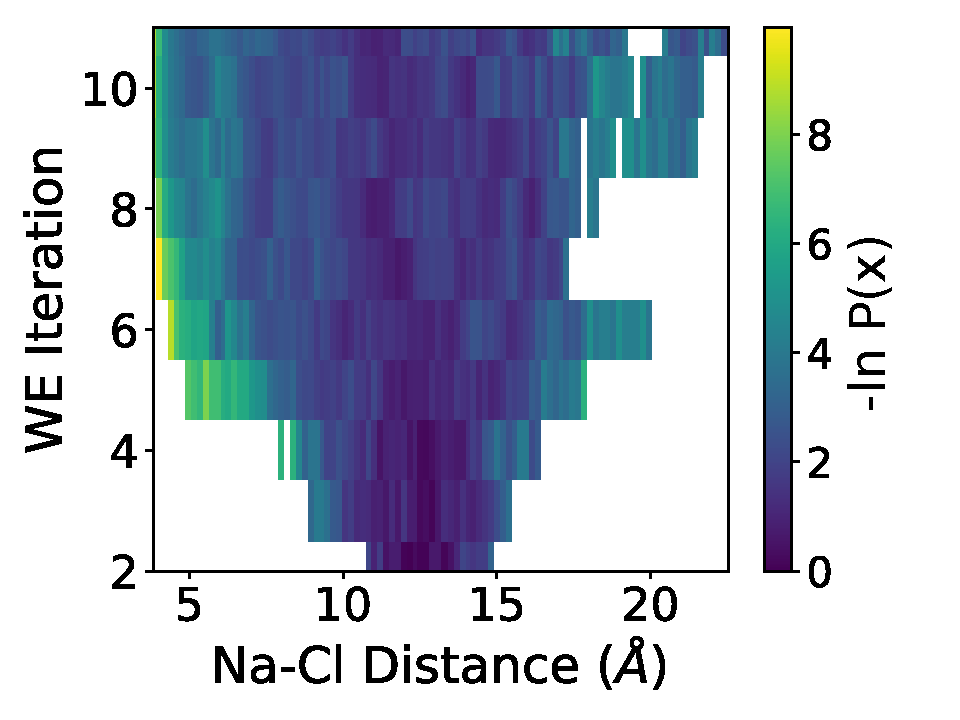
\includegraphics[width=\linewidth]{figures/Figure4-2.pdf}
\caption{Probabiity evolution of Na\textsuperscript{+}/Cl\textsuperscript{-} association as a function of interatomic distance and WE iteration. 
The distribution from your particular simulation may look slightly different. 
Observe that at the beginning of the simulation, the probability is centered around 12 \AA{} (the initial distance).}
\label{fig:nacl-hist}
\end{figure}
%%%%%%%%

As expected, most of the probability at the start of our simulation is concentrated around the progress coordinate value for our initial state (10 \AA). 
As our simulation progresses, the probabilities fan out in both directions, with most of the probabilities moving towards larger values and some of the probabilities nearing our target value of 2.6 \AA. 
To see if your simulation has generated some successful binding events after only 10 iterations, run the following:
\begin{verbatim}
  $ w_succ
\end{verbatim}
 
The example simulation had its first successful event after 14 iterations. 
The output will show (if a successful event occured) the iteration and segment number in which the first event occurred (e.g. iteration 14, segment 2).

You can trace this successful trajectory back to the basis state to obtain a complete trajectory with the \verb|w_trace| command. 
You will need to provide the iteration and segment of the successful trajectory as options separated by a colon:
\begin{verbatim}
  $ w_trace 14:2
\end{verbatim} 
The output will be written to the file \verb|traj_14_2_trace.txt|. 
That file contains the parents of the successful trajectory all the way back to the basis state. 

\subsubsection{Analyzing the WE Simulation}
\label{tut:basic-nacl-plot}
One way to assess the convergence of our simulation is to determine when the primary observable of interest (i.e. the flux into the target state) levels off. 
To monitor the flux, we will first need to prepare our \verb|west.cfg| file to analyze the simulation. 
This is normally done by adding an analysis module to the end, which is already present in this tutorial’s files. 
Use this as a template for future analyses.

You will see that we create an analysis instance called \verb|TEST| and then define bins and states for this scheme. 
These bins are strictly for analysis and have nothing to do with our progress coordinate bins defined earlier. 
Since we only need to designate the bound and unbound states here, we define three bins: 
\begin{verbatim}
  [0.0, 2.6, 10.0, ‘inf’]
\end{verbatim}
 
The way that state definitions work is that you provide a progress coordinate in the configurational space and whichever analysis bin that coordinate is in becomes that state. 
For instance, our bound state definition is given by \verb|[0]|, so whichever bin above that the value 0 falls into will be our “bound” state. 
This is the bin from 0 to 2.6. 
The same goes for the unbound state (10.0 to infinity). 
The intermediate state (2.6 to 10.0) does not need to be defined.

With these states defined we can now analyze how much probability, in the form of trajectory weight, is entering or leaving each state using the \verb|w_ipa| program, which will run two separate WESTPA tools, \verb|w_assign| and \verb|w_direct|. 
To generate the H5 files needed to analyze the fluxes, run the following from the main simulation directory:

\begin{verbatim}
  $ w_ipa -ao
\end{verbatim}

You will see that a new directory titled \verb|ANALYSIS| has been created, inside of which is a subdirectory corresponding to our \verb|TEST| analysis scheme that was defined in the \verb|west.cfg| file. 
Inside of this subdirectory are our \verb|assign.h5| and \verb|direct.h5| files. 
The \verb|direct.h5| file is where the fluxes are stored. 
We can open it up with \verb|hdfview| and view all of the datasets.
 
The \verb|target_flux_evolution| dataset gives the flux over time (number of WE iterations) into each state we defined earlier. 
To view this dataset, double click on it. 
The 0th column corresponds to the flux into state 0, which we defined as our target state. 
The iter stop is at the beginning of that iteration, so if you had a binding event by iteration 10, observe the  flux into our target state. 
Highlight the “expected” column and click the plotting button in the upper-left hand corner to view the flux evolution as a function of 0-indexed iteration.
 
By iteration 10, the flux has most likely not levelled off, so our simulation cannot be considered converged. 
Let’s continue the simulation for a total of 100 WE iterations and analyze the resulting dataset. 
A completed H5 file is included in the \verb|for_analysis/| directory for your convenience.
Your plot should look something similar to \textbf{Figure \ref{fig:nacl-flux}}, which was generated in \verb|matplotlib|. 

%%%Fig 5%%%
\begin{figure}[t]
\centering
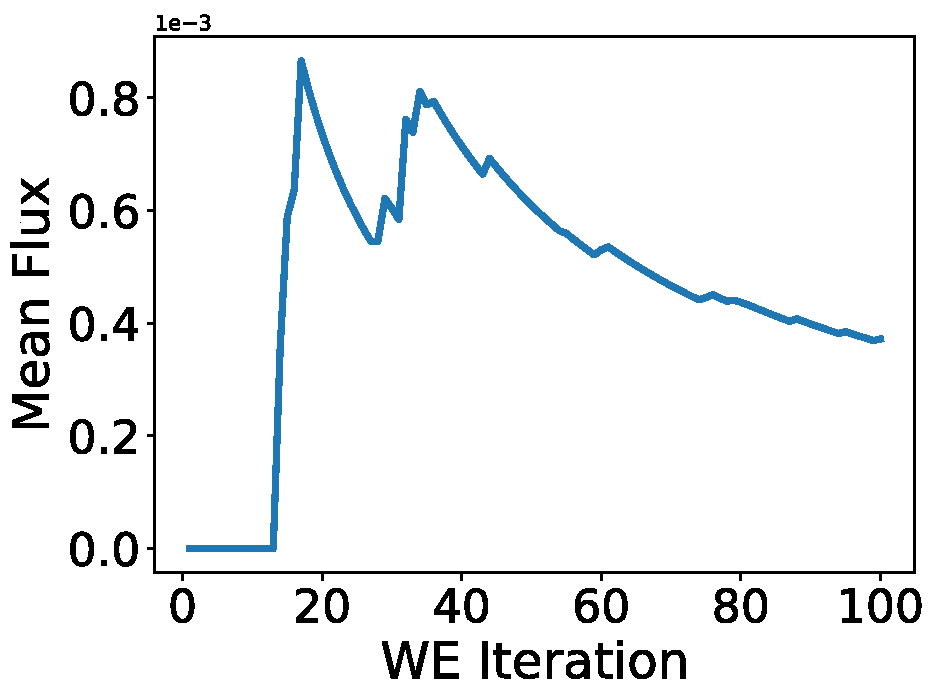
\includegraphics[width=\linewidth]{figures/Figure5-2.pdf}
\caption{Mean flux evolution of Na\textsuperscript{+}/Cl\textsuperscript{-} association as a function of WE iteration. 
The mean flux alternatively rises sharply and then relaxes. 
These "peaks" correspond to probability crossing into the target state. 
Your plot may still not be completely converged after 100 WE iterations.}
\label{fig:nacl-flux}
\end{figure}
%%%%%%%%

While the flux into the target state has not completely levelled off, it is much more steady than previously, so we can stop the simulation here and consider how much longer we should extend the simulation. 
For other systems, you may want to run the simulation longer for better convergence. 
You may also want to have additional criteria for convergence.

To visualize a trajectory, one must first identify a continuous series of trajectory segments in each iteration from the basis state to the target state. 
This will be given in the \verb|w_succ| output along with \verb|w_trace|, as we have done previously. 
However, you will also need to retrieve the trajectory file from each of those segments and combine them using \verb|cpptraj|. 
To automate this process, we have provided the \verb|amberTraj.sh| script, which can be adapted for other systems. 
This script uses the \verb|cpptraj| program available in AmberTools to extract the binding trajectory of a successful event.
The resulting trajectory file can be loaded along with the system topology into the VMD visualization software to generate a movie of the association process.
 
\subsubsection{Conclusion}

Hopefully by this point you have gained a good idea of the work flow required to set up, run, and analyze a WESTPA simulation using a simple progress coordinate. 
If you desire more complex options for your simulations (e.g. multi-dimensional progress coordinates) and further discussion of how to choose various simulation parameters, we highly suggest going through the other tutorials to get a sense of how that can be done.

\subsection{Intermediate Tutorial: P53 Peptide Conformational Sampling}
\label{tut:p53-int}

\subsubsection{Introduction}

Since the WE algorithm aims to fill empty bins in configurational space, WE simulations can be effective in the enhancement of conformational sampling \citep{Zwier2015} as well as the generation of pathways and rate constants for rare events. 
This tutorial will focus on the conformational sampling of a peptide and instruct users on how to set up and analyze a simulation involving a two-dimensional progress coordinate. 
In addition, we will go over how the binning scheme can be chosen and adjusted in order to balance efficiency and performance.

\textbf{Learning Objectives.} This tutorial will help users develop a sense for which progress coordinates may be effective for conformational sampling of a peptide and how to bin along those progress coordinates.  

Specific learning objectives include:
\begin{enumerate}
\item How to set up a two-dimensional progress coordinate
\item How to monitor this coordinate as the simulation progresses
\item How to evaluate whether the binning scheme is effective
\item Combining and creating bins “on-the-fly”
\item Storing and accessing auxiliary data
\end{enumerate}

\subsubsection{Prerequisites}

Users should have completed the \textbf{Basic Tutorial \ref{tut:nacl-basic}} and have a potential progress coordinate in mind for their system of interest. 

\textbf{Computational Requirements.} This simulation required at least 10 GB of disk space and \textasciitilde 36 hours to complete (40 iterations) on a 12-core, 2.6 GHz Intel Xeon node.
This tutorial uses AmberTools19’s \verb|sander| package for dynamics propagation and the  \verb|cpptraj| package for progress coordinate calculations (\url{http://ambermd.org/AmberTools.php}).  
AmberTools is available free of charge.

\subsubsection{Adding Another Dimension to the Progress Coordinate}

While a one-dimensional progress coordinate can be effective for molecular association processes (e.g. Na\textsuperscript{+}/Cl\textsuperscript{-} in the \textbf{Basic Tutorial}), a two-dimensional coordinate may be necessary for more complex processes such as peptide/protein conformational transitions. 
To add another dimension to the progress coordinate, we first specify the progress coordinate dimensionality as “2” in the \verb|west.cfg| file. 
Next, we calculate the values corresponding to each dimension of the progress coordinate and pass the resulting two values at the same time to \verb|$WEST_PCOORD_RETURN| in both the \verb|get_pcoord.sh| and \verb|runseg.sh| scripts. 
For example, if the first dimension of the progress coordinate has a value of 1 and the second dimension has a value of 5, (1 5) must be passed at the same time to \verb|$WEST_PCOORD_RETURN| instead of sequentially as 1 and then 5. 
This can be done with the \verb|paste| command in bash (see example \verb|get_pcoord.sh| and \verb|runseg.sh| files). 
In addition, the bins will need to be specified as two lists, one for each of the two dimensions.
This is done by adding dashed entries (one underneath the other) in the \verb|west.cfg| section for bin definitions. 
A user may alternatively choose to define a two-dimensional binning scheme in a \verb|system.py| file.

\subsubsection{Preparing the WE System}
\label{tut:p53-int-prep}

\textbf{The System.} We will focus on  the conformational sampling of a 15-residue, N-terminal peptide fragment of tumor suppressor p53 that has been thought to be disordered in its unbound state and adopts an $\alpha$-helical conformation upon binding the MDM2 protein. 
Simulations were run at 275 K using the Amber ff14SBonlysc force field \citep{ff} and generalized Born implicit solvent \citep{implicit_solvent}. 
As in the Basic Tutorial, we will not go into detail about how the files were generated in Amber or the decisions made in setting up the system with Amber.

\textbf{Choosing an Initial State.} Our WE simulation will be started from the MDM2-bound conformation of the p53 peptide. 
In particular, coordinates for the peptide conformation will be extracted from the crystal structure of the MDM2-p53 peptide complex \citep{Kussie1996}. 
This $\alpha$-helical conformation of the peptide will then be energy-minimized and equilibrated before subjecting the resulting, solvated system to a WE simulation.

\textbf{Files for Dynamics.} The topology file (\verb|P53.MDM2.prmtop|) and dynamics input file (\verb|md.in|) can be found in the \verb|common_files/| directory. 
In the \verb|md.in| file, it should be specified that the trajectory segment will be run for a length that corresponds to a $\tau$ value of 50 ps.

\textbf{Preparing the Simulation Environment.} See the corresponding subsection in the \textbf{Basic Tutorial \ref{tut:nacl-basic}}.

\textbf{Equilibrium vs Steady State WE.} In the \verb|init.sh| file, observe that all lines mentioning \verb|TSTATE_ARGS| have been removed. 
This signals WESTPA to run an equilibrium WE simulation in which we do not have a set target state. 
This is a good option when the goal of your process is to generate as many configurations as possible and you have no set target state in mind.

\textbf{Progress Coordinate, Binning Scheme and $\pmb{\tau}$ Value.} To extensively sample the conformations of the peptide, we might define a progress coordinate that monitors the extent of “unfoldedness” in the peptide using the RMSD of a given conformation from the initial structure. 
However, RMSD cannot differentiate among conformations that have the same large RMSD values. 
To further differentiate between such conformations, we can include another orthogonal measure of unfoldedness such as the end-to-end distance of the peptide. 

To determine a suitable binning scheme, we will start with an upper limit of 10 \AA{} for the heavy-atom RMSD dimension of the progress coordinate. 
Spacing the bins along this dimension by 1’s may be too large for any transitions to occur between bins so we opt for a finer bin spacing:
\begin{verbatim}
  [0.0, 0.2, 0.4, 0.6, 0.8, 1.0, 1.4, 1.8,
   2.2, 2.6, 3.0, 3.5, 4.0, 5.0, 6.0, 7.0,
   8.0, 9.0, 10.0, ‘inf’]
\end{verbatim}
We will see how the trajectories progress and adjust accordingly. 
Notice that a bin spacing of 0.2 is not maintained for the entire length, as 50 bins even along one dimension would result in a very large number of total trajectories (4 trajectories per bin would yield a total of 200 trajectories if all of the bins are occupied). 
Furthermore, care must be exercised in the addition of bins along a second dimension as the total number of trajectories can “blow up” to an enormous number of trajectory segments (e.g. 10,000).

To get a feel for how the end-to-end distance evolves in the simulation, let’s expand out from the initial distance of 28.5 \AA{} with 0.5-\AA{} wide bins in either direction:
\begin{verbatim}
  [0, 20, 20.5, 21, 21.5, 22, 22.5, 23, 23.5,
   24, 24.5, 25, 25.5, 26, 26.5, 27, 27.5, 28,
   28.5, 29, 29.5, 30, 30.5, 31, 31.5, 32, 32.5,
   33, 33.5, 34, 34.5, 35, 35.5, 36, ‘inf’]
\end{verbatim}
Our $\tau$ value should allow for successful transitions between bins of this spacing.

\textbf{Other WE Parameters.} Let’s run our WE simulation with 4 trajectories/bin for 40 iterations. 
Since the goal here is the conformational sampling of a peptide and we are running an equilibrium WE simulation, we do not need to define a target state.

%%%Fig 6%%%
\begin{figure}[ht]
\centering
\begin{subfigure}[A]{0.35\textwidth}
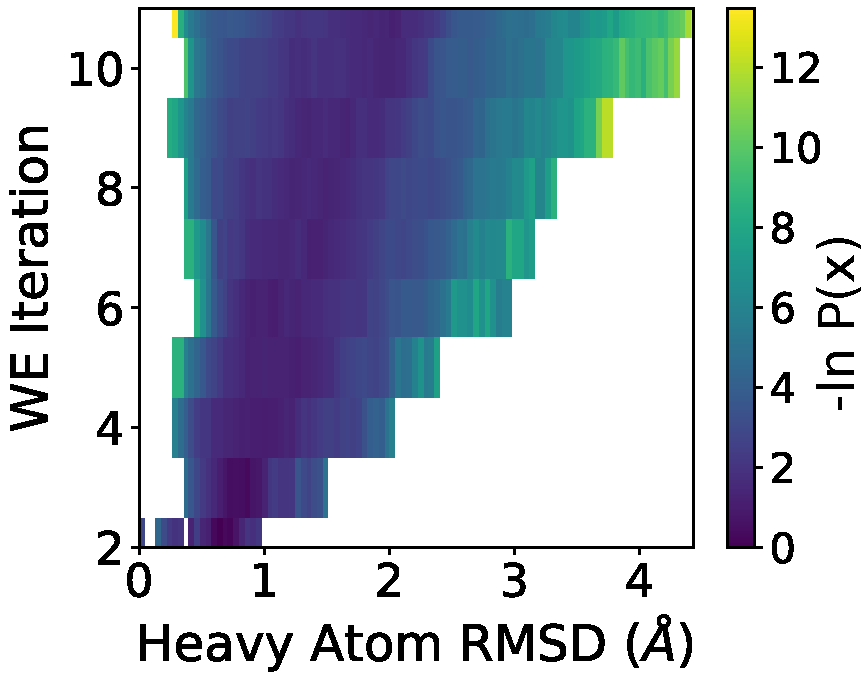
\includegraphics[width=\linewidth]{figures/Figure6A-2.pdf}
\end{subfigure}
\begin{subfigure}[B]{0.35\textwidth}
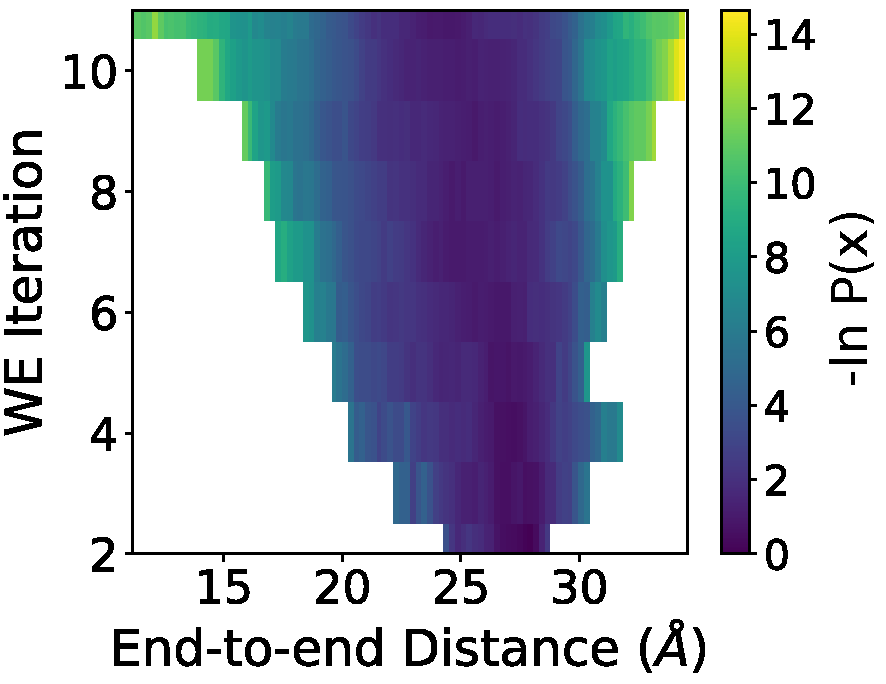
\includegraphics[width=\linewidth]{figures/Figure6B-2.pdf}
\vspace{-0.5cm}
\end{subfigure}
\caption{Probability distributions for each of the two progress coordinate dimensions versus WE iteration for the p53 system. 
The simulation was analyzed after 10 WE iterations.}
\label{fig:p53-hist-10}
\end{figure}
%%%%%%%%

\subsubsection{Tracking the Auxiliary Data}

While it is possible to go back after a simulation has run and calculate some value you wish you had kept track of, it can be tricky to do so (though possible with a tool called \verb|w_crawl| which is not discussed in this guide). 
We strongly recommend conducting all relevant analysis during the simulation and storing the resulting data as auxdata in the H5 file. 
In our case, we will  calculate and store the $\phi$/$\psi$ backbone dihedral angles of the peptide as auxdata for each of the sampled conformations.  

To signal for WESTPA to collect auxdata, you will need to add an auxiliary dataset into the \verb|west.cfg| file and make sure it is enabled. 
See the \verb|west.cfg| file in the tutorial directory for an example of how this might look. 
You can name the dataset whatever you would like. 

Once you have specified the datasets and named them, you will need to add in commands to \verb|runseg.sh| that calculate those values and pass them to WESTPA system variables. 
The variables will be named \verb|$WEST_XYZ_RETURN| where “xyz” is the name given to the dataset in the \verb|west.cfg| file. 
This can be treated analogously to the pcoord value and \verb|$WEST_PCORD_RETURN|.

\subsubsection{Initializing and Running the WE Simulation}

Make sure that your \verb|get_pcoord.sh| and \verb|runseg.sh| files are calculating the RMSD and end-to-end distance and returning these values to \verb|$WEST_PCOORD_RETURN|. 
The \verb|get_pcoord.sh| script will calculate the initial progress coordinates using AmberTools’ \verb|cpptraj| program from within the script, as opposed to reading the value from an external file as in the \textbf{Basic Tutorial \ref{tut:nacl-basic}}.
The \verb|runseg.sh| uses AmberTools’ \verb|sander| program for dynamics propagation and does so within the script.

\subsubsection{Monitoring the WE Simulation (10 Iterations)}

Once the simulation has run for about 10-20 iterations, copy the H5 file and run \verb|w_pdist| with the copied file. 
You can then use \verb|plothist| to view each dimension of the progress coordinates separately as the values evolve over the course of those few iterations:
\begin{verbatim}
  $ plothist evolution pdist.h5 0 -o hist_dim0.pdf
  $ plothist evolution pdist.h5 1 -o hist_dim1.pdf
\end{verbatim}

Where the “0” or “1” after the \verb|plothist| command is the progress coordinate dimension (zero indexed). 
Observe the two probability distributions in \textbf{Figure \ref{fig:p53-hist-10}}.

\subsubsection{Adjusting Bin Spacings "On the Fly"}

The RMSD has reached a value of 4-5 \AA{} and the end-to-end distance has reached \textasciitilde 10 \AA{}, which is encouraging progress for only 10 iterations. 
Note that most of the probability (and therefore most of the computation) is still stalled in the initial states of 1-2 \AA{} RMSD and 20-25 \AA{} end-to-end distance. 
We can help  focus the computing power on the more interesting “edge” conformations by modifying the binning scheme before continuing the simulation.
  
In WESTPA, the binning scheme can be updated at any time since the trajectory weights are independent of the bins (and progress coordinate). 
To do so, first stop the simulation and then adjust the bins in your \verb|west.cfg| file. 
Re-start your simulation by running the \verb|run.sh| script again and the simulation will continue from where it left off. 
At the start of the next iteration, the new bins will have been implemented.  

In our case, I would like to focus sampling on higher RMSD values (3-4 \AA) instead of those \textasciitilde 1-2 \AA. 
To do this, I will collapse the bins from 0 to 1.8 \AA{} and define some more bins past 10 \AA:
\begin{verbatim}
  [0.0, 1.8, 2.2, 2.6, 3.0, 3.5, 4.0, 5.0, 6.0, 7.0
   8.0, 9.0, 10.0, 11, 12, 14, 16, 18, 20, ‘inf’]
\end{verbatim}

For the end-to-end distance, I will add more bins for the lower distances and collapse bins over 26 \AA. 
We would normally want to keep these bins over 26 \AA{} but having fewer will shorten the runtime of this tutorial.
\begin{verbatim}
  [0, 2, 4, 6, 8, 10, 12, 14, 16, 18, 20, 21,
   22, 23, 24, 25, 26, ‘inf’]
\end{verbatim}

The reason we eliminated the initial 0.5 \AA{} spacings is that this degree of freedom is readily explored in the system.

 %%%Fig 7%%%
\begin{figure}[t]
\centering
\vspace{-0.25cm}
\begin{subfigure}[A]{0.35\textwidth}
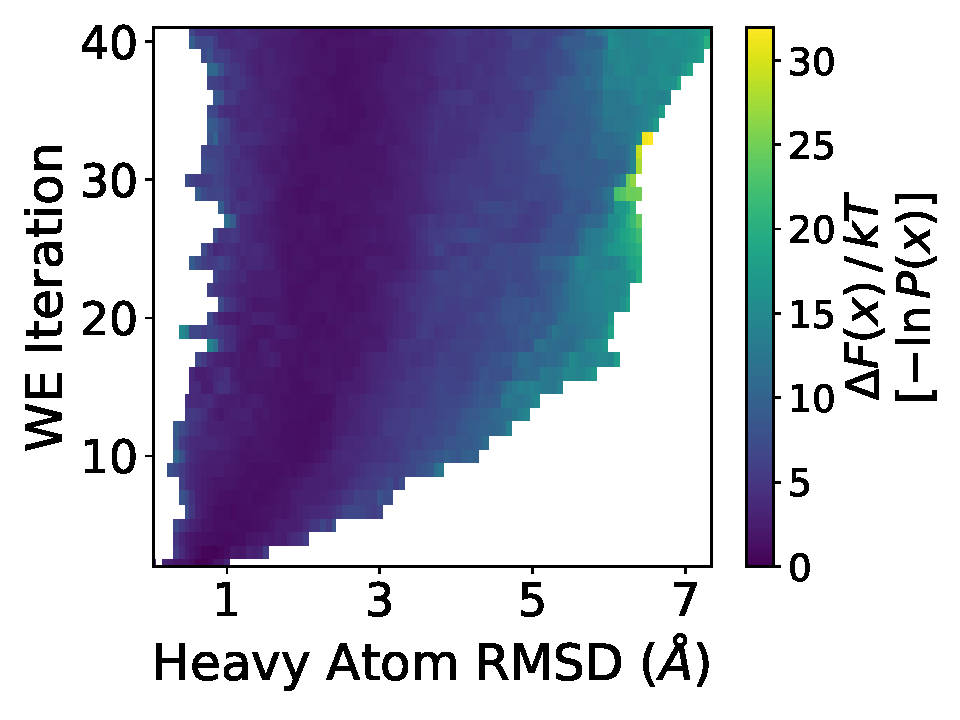
\includegraphics[width=\linewidth]{Figure7A.pdf}
\vspace{-0.75cm}
\end{subfigure}
\begin{subfigure}[B]{0.35\textwidth}
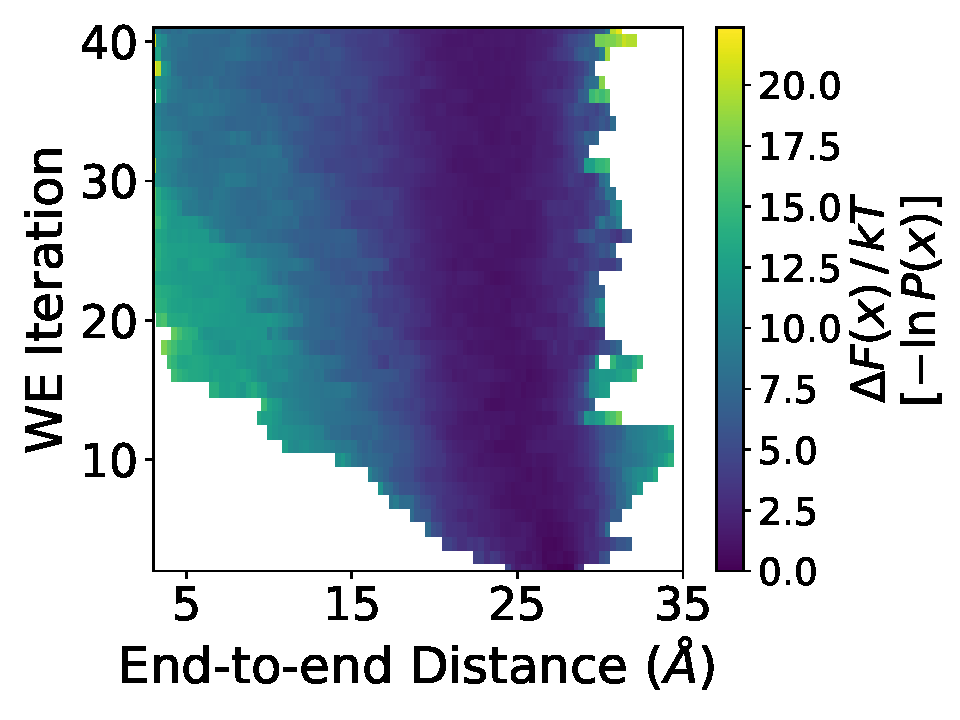
\includegraphics[width=\linewidth]{Figure7B.pdf}
\end{subfigure}
\vspace{-0.75cm}
\caption{Probability distributions for each of the two progress coordinate dimensions versus WE iteration for the p53 system. 
The simulation was re-analyzed after 40 WE iterations}
\label{fig:p53-hist-40}
\vspace{-0.25cm}
\end{figure}
%%%%%%%%

\subsubsection{Monitoring the WE Simulation (40 Iterations)}

After running the simulation for another 30 iterations (for a total of 40), we obtained the following updated probability distributions displayed in \textbf{Figure \ref{fig:p53-hist-40}}.
The completed H5 file is included in \verb|for_analysis/| for your convenience.

The effects of the bin-modifications can clearly be seen in the case of the end-to-end distribution. 
No more trajectories with an end-to-end distance >30 \AA{} can be seen after iteration 10, a result of the choice not to bin over 26 \AA{} in that dimension.

The end-to-end distance seems to have reached 2-3 \AA{} around iteration 20. 
The RMSD plateaued a bit from iterations 20-30 but then proceeded to values around 7 \AA.  
Two lessons can be learned from these observations. 
First, if you do not have bins in a particular direction, you may not see sampling in that direction. 
Second, even though the RMSD coordinate appeared to have stalled around iteration 20-30, it eventually was able to surmount whatever barrier existed and attain some higher RMSD values. 
Patience is key, as a single trajectory may replicate to become many trajectories if it crosses into a new bin.

%%%Fig 8%%%
\begin{figure}[t]
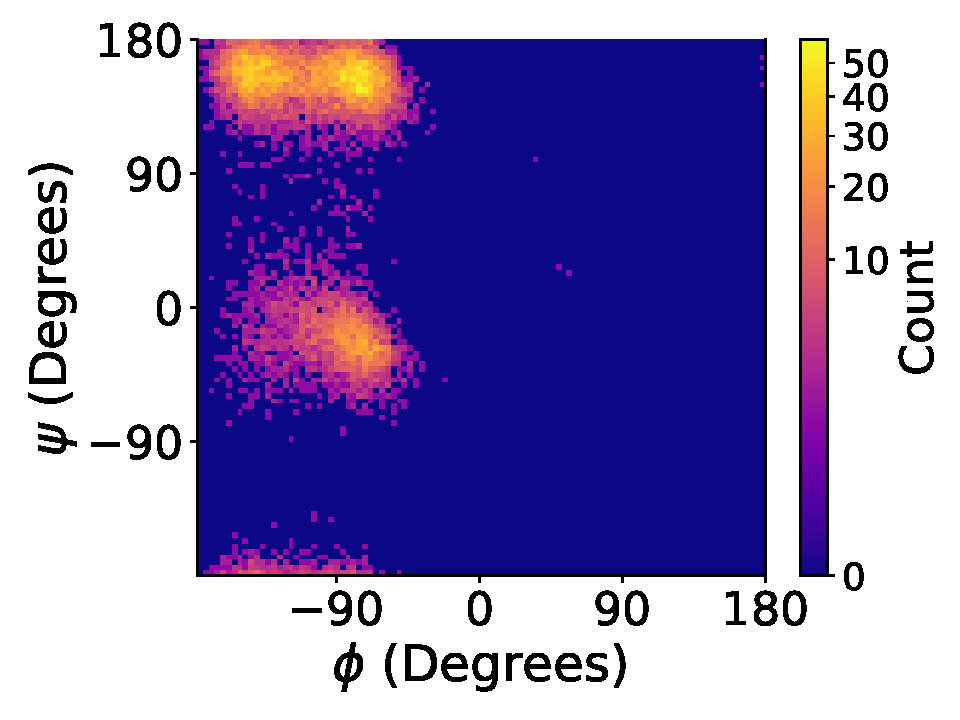
\includegraphics[width=\linewidth]{Figure8.pdf}
\vspace{-0.75cm}
\caption{Ramachandran plot showing the occurance of $\phi$/$\psi$ angles of the second peptide bond of the p53 peptide, for each WE segment throughout the course of the simiulation.}
\label{fig:p53-rama}
\vspace{-0.25cm}
\end{figure}
%%%%%%%%

\subsubsection{Accessing Auxiliary Data}

To access the auxdata from the H5 file, you can open \verb|west.h5| in \verb|hdfview| but this will not allow you really use the data. 
To plot all of the dihedrals as a Ramachandran plot in \verb|matplotlib| as shown in \textbf{Figure \ref{fig:p53-rama}} (actually, we just did so for the second dihedral, but you could extend it to all if you so desire), you will need to utilize the \verb|h5py| package in Python to extract the auxdata values from the \verb|west.h5| file and then plot them. 
The plotting script is included in the tutorial directory.

\subsubsection{Conclusion}

Users should now be familiar with setting up a two-dimensional progress coordinate and working with auxiliary data. 
These two "tools" will help to expand your repertoire of WESTPA simulation techniques and give you access to more complex and informative simulations. 
Users should also now be familiar with changing bin spacings “on-the-fly” as well. 

\subsection{Intermediate Tutorial: Folding of Chignolin Mini-Protein}
\label{tut:chig-int}

\subsubsection{Introduction}

Protein folding processes have been challenging to simulate due to the relatively long time scales involved. 
In this tutorial, we will use WESTPA to simulate the folding and unfolding of the chignolin mini-protein and to calculate the corresponding rate constants. 
We will run steady-state WE simulations of chignolin folding and unfolding processes separately. 
We will also compare the results of these simulations with those from brute force MD simulations, demonstrating the correctness and potential usefulness of the WE strategy. 
 
\textbf{Learning Objectives.} This tutorial demonstrates how steady state WE simulations can be used to generate pathways and rate constants for both protein folding and unfolding processes.  

Specific learning objectives include:
\begin{enumerate}
\item How to use brute force simulations to identify appropriate initial and/or a target states
\item How to obtain the probability flux into the target state of a WESTPA simulation, how to convert it to a mean rate constant, and how to interpret the results
\end{enumerate}

\textbf{Prerequisites.} Users should have completed the \textbf{Basic Tutorial \ref{tut:nacl-basic}}.
 
\textbf{Computational Requirements.} We note that significantly more computing time is required for the folding simulations to yield converged rate constants and hence we suggest the user should start with the unfolding simulations. 
In particular, the WE unfolding simulation required \textasciitilde 53 hours for 1000 iterations on 32 CPU cores of 2.6 GHz Intel Xeon processors (\textasciitilde 5 GB of disk space) while the WE folding simulation required \textasciitilde 8 days for 10,000 iterations (200 ns of molecular time) using the same resource (\textasciitilde 50 GB of disk space).
To become familiar with setting up and running the WE simulations, the users can carry out several iterations.  Also, the brute-force simulation described below can be performed for tens of ns, as we benchmarked this system to produce \textasciitilde 150 ns per day on one of the above-mentioned CPUs. Output files for 1000 iterations of the WE unfolding and 10000 iterations of the WE folding simulations (as well as for 4 us of the brute-force simulation) can be found in the corresponding subdirectories. These files should be used for the analysis procedures outlined below.
This tutorial uses AmberTools19’s \verb|sander| package for dynamics propagation and the  \verb|cpptraj| package for progress coordinate calculations (\url{http://ambermd.org/AmberTools.php}). 
AmberTools is available free of charge.

\textbf{The System.} The chignolin mini-protein with the sequence GYDPETGTWG forms a $\beta$-hairpin and folds/unfolds on a timescale that is accessible to brute force simulations, which provide a reference data set for comparison with WESTPA results. 
The folded chignolin structure (PDB code: 1UAO, \citep{Honda2004}), serves as the starting structure for both the brute-force and WE unfolding simulations. 
Both dynamics propagation and simulation analysis are carried out using the Amber software package. 
Simulations were run at 275 K using the Amber ff14SBonlysc force field \citep{ff} and generalized Born implicit solvent \citep{implicit_solvent}. 

\subsubsection{Brute Force Simulations}

\textbf{Overview.} As mentioned in \textbf{Section \ref{intro:prereq}}, it is important to run multiple, short, brute force simulations prior to using WESTPA. 
In the case of chignolin, which both folds and unfolds on timescales accessible to brute force simulation, brute force simulations can provide information on defining the unfolded and folded states. 
 
\textbf{Running and Analyzing the Brute Force Simulation.} We perform a 4-$\mu$s brute force simulation of chignolin and write out coordinates every 20 ps. 
All files can be found in the \verb|brute_force/| directory. 
The user can change these parameters in the MD config file \verb|md.in|. 
The simulation can be submitted with the following command:

\begin{verbatim}
  $ ./run.sh
\end{verbatim}
 
This submission script may have to be adjusted to the user’s computing platform.

The chignolin C\textsubscript{$\alpha$} RMSD can be computed in the following way:

\begin{verbatim}
  $ cpptraj chignolin.prmtop < get_rmsd.in
\end{verbatim}

This command assumes the brute force simulation trajectory as well as the chignolin parameter topology and folded structure pdb files are all in the current directory.

The output RMSD data file, \verb|rmsd.dat|, lists the time evolution of the chignolin C\textsubscript{$\alpha$} RMSD over the course of the simulation (each line corresponds to a frame). 

\textbf{Figure \ref{fig:chig-rmsd}} shows the C\textsubscript{$\alpha$} RMSD over simulation time for a brute-force simulation that started from the folded $\beta$-hairpin, revealing several unfolding and refolding events within 4 $\mu$s. 
The unfolded and folded states are defined by visual inspection of the RMSD plot and simulated conformations, which show a fully formed $\beta$-sheet and native hydrogen bonds at RMSD < 0.5 \AA{} and a disrupted $\beta$-sheet with broken native hydrogen bonds at RMSD > 4 \AA{} (this pair of RMSD values will also be used later to define target states in WESTPA simulations).  
Note that the (un)folding rate constants will be sensitive to the state definitions, and defining states is a challenging process beyond the scope of this tutorial. 
Our state definitions are designed to avoid potential recrossing artifacts in rate calculations: once a trajectory reaches a state it should tend to remain there, rather than immediately returning to the previous state.
 

%%%Fig 9%%%
\begin{figure}
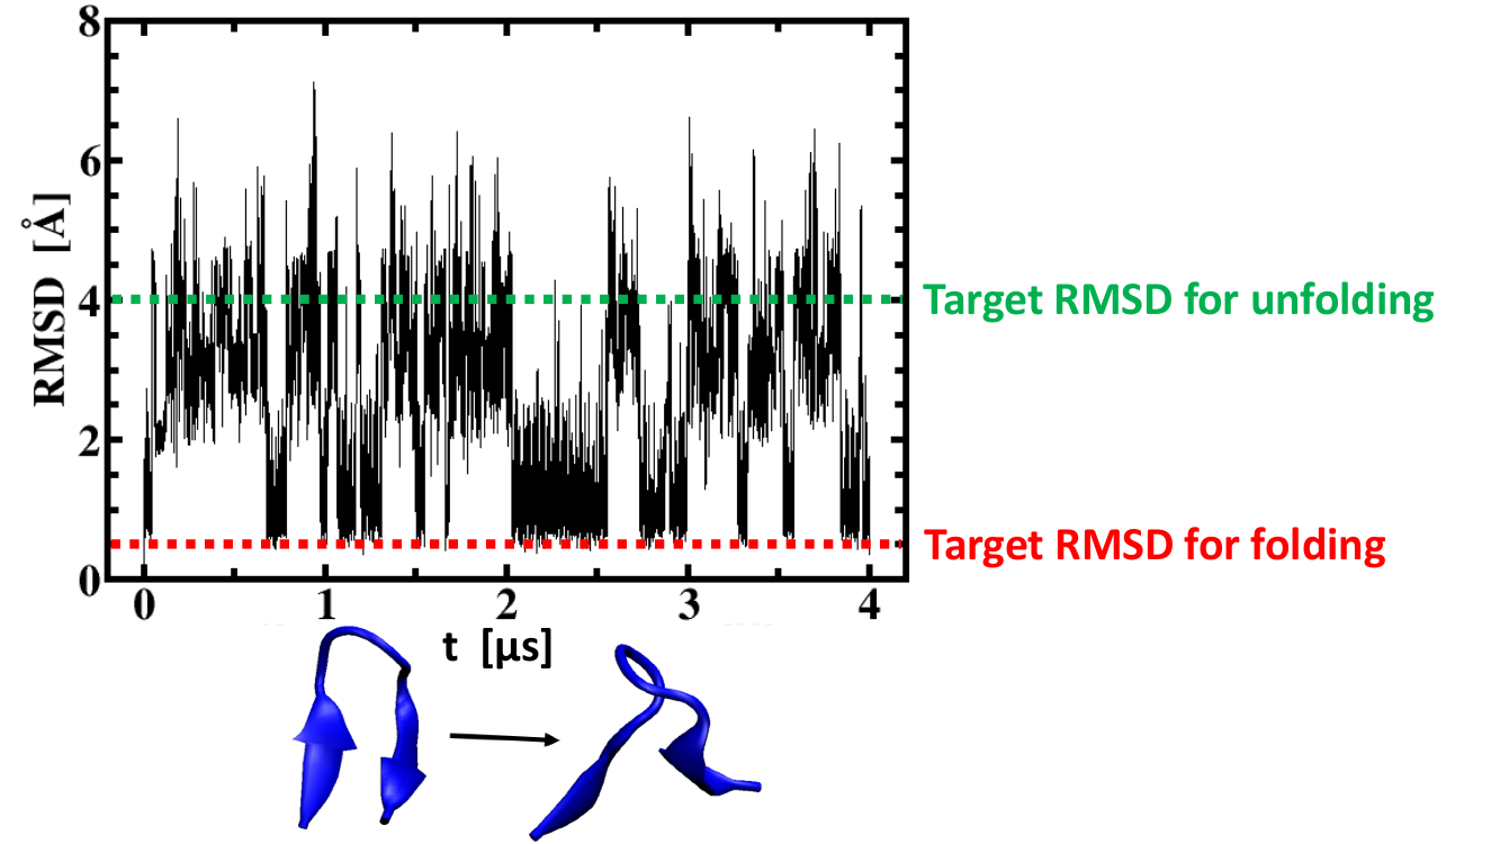
\includegraphics[width=\linewidth]{Figure9.png}
\caption{C\textsubscript{$\alpha$} RMSD vs simulation time for the brute force simulation of chignolin.}
\label{fig:chig-rmsd}
\vspace{-0.25cm}
\end{figure}
%%%%%%%%

According to the Hill relation \citep{Hill1989}, the rate constant is exactly the inverse mean first-passage time (MFPT) of the underlying process, where, for instance, the FPT for unfolding is the time required to reach the unfolded state (RMSD > 4 \AA) after first folding (RMSD < 0.5 \AA). 
The user can run the following to obtain the MFPTs for both the folding and unfolding processes: 
\begin{verbatim}
  $ python get_mfpt.py rmsd.dat 20e-12 0.5 4.0
\end{verbatim}

The command-line arguments are the RMSD data file, time interval at which the RMSD values are calculated in seconds, and threshold RMSD values for the folded and unfolded states in Angstroms. 
The rate constant of unfolding is estimated to be 0.13 x 108 s\textsuperscript{-1} (credibility region: 0.09 x 108 s\textsuperscript{-1} – 0.18 x 108 s\textsuperscript{-1}) and that of folding is estimated to be 0.71 x 107 s\textsuperscript{-1} (credibility region: 0.44 x 107 s\textsuperscript{-1} – 1.24 x 107 s\textsuperscript{-1}). 
Credibility regions are derived from a Bayesian bootstrapping procedure \citep{mostofian_statistical_2019}. 

\subsubsection{Using WESTPA}

\textbf{Overview.} We will carry out separate steady-state WE simulations for the unfolding and folding processes. 
This strategy is not only more efficient than equilibrium WE simulations in estimating rate constants (see \textbf{Section \ref{tut:basic-nacl-3}}), but enables us to set WE parameters for each process (e.g. bin spacing) in a more process-specific way if needed. 
The target state of the folding simulation will be used as the initial state of the unfolding simulation and vice versa. 

\textbf{Choosing an Initial State.} As done for the brute force simulations, WE simulations of the unfolding process will be started from the NMR structure of chignolin. 
WE simulations of the folding process will be started from an unfolded conformation of chignolin (RMSD > 4 \AA) that has been generated by the above brute force simulations.
 
\textbf{Files for Dynamics.} All files are in the \verb|common_files/| subdirectory of either the \verb|WE_folding/| or the \verb|WE_unfolding/| directory.
 
\textbf{Preparing the Simulation Environment.} See the corresponding subsection in \textbf{Basic Tutorial \ref{tut:nacl-basic}}.
 
\textbf{Equilibrium vs Steady State WE.} Here we will run separate steady state WE simulations of the folding and unfolding processes, defining a target state (\verb|TSTATE_ARGS|) in the \verb|init.sh| files.

\textbf{Progress Coordinate, Binning Scheme and $\pmb{\tau}$ value.} As mentioned above, we will use a one-dimensional progress coordinate consisting of the C\textsubscript{$\alpha$} RMSD from the folded structure of chignolin. 
Although the RMSD with respect to a single reference structure may not be an ideal coordinate for distinguishing between  various conformation, it proves sufficient for our example. 
Folded and unfolded states are defined based on maximum and minimum RMSD values, respectively, that have been sampled by the above brute force simulations. 
We will use a bin spacing  of 0.2 \AA{} and a $\tau$ value of 20 ps. 
However, the very first bin for the unfolding simulations is larger than the regular bin width with RMSD = [0 \AA, 0.5 \AA] because any structure with RMSD < 0.5 \AA{} is considered to be in the folded initial state. 
Analogously, for the folding simulations, the very last bin is larger than the regular bin width of 0.2 \AA. 
\pagebreak  

\textbf{Other WE Parameters.} As done in the previous tutorials, our WE simulations were carried out using 4 trajectories/bin. 
The unfolding and folding simulations were run for 1000 and 10,000 WE iterations, respectively, in order to reach a steady value of the corresponding rate constants. 
 
\textbf{Initializing and Running the WE simulations.} The \verb|init.sh| and \verb|run.sh| files can be found in the corresponding directories for both WESTPA simulations. 
The RMSD progress coordinate is calculated and its values returned to \verb|$WEST_PCOORD_RETURN|.   

\textbf{Monitoring and Analyzing the WE Simulations.} To compute the rate constant for the folding or unfolding process, we first calculate the mean probability flux into the target state by running the following WESTPA analysis tool:
\begin{verbatim}
  $ w_fluxanl
\end{verbatim}
The output is the H5 file \verb|fluxanl.h5|, which contains the instantaneous probability flux into the target state for each iteration. 
The following Python script calculates, for any WE iteration, the average rate constant based on the corresponding probability flux arriving in the target state over a preceding window of molecular simulation times (e.g., over 1 ns):
\begin{verbatim}
  $ python get_mean_rate.py 20e-12  1e-9
\end{verbatim}

The command-line arguments are the $\tau$ value and the time width for window-averaging. 
Both arguments are in units of seconds.
 
\textbf{Figure \ref{fig:chig-flux}} shows the evolution of the average unfolding rate constant of chignolin as a function of molecular time for three independent WE simulations. 
After a few ns, the average rate constants for all of these simulations have leveled off and are roughly comparable to that derived from brute force simulations. 
One difference between the WE and brute force simulations is that the former estimates the MFPT based on the chosen initial structure(s) which may not correspond precisely to the ensemble of starting structures implicit in extracting first-passage events from brute force simulations. 
Note that a three-fold difference in the rate constants among the three WE simulations amounts to only \textasciitilde 0.6 kcal/mol difference in the effective free energy barrier to unfolding (at the simulation temperature of 275 K).

%%%Fig 10%%%
\begin{figure}
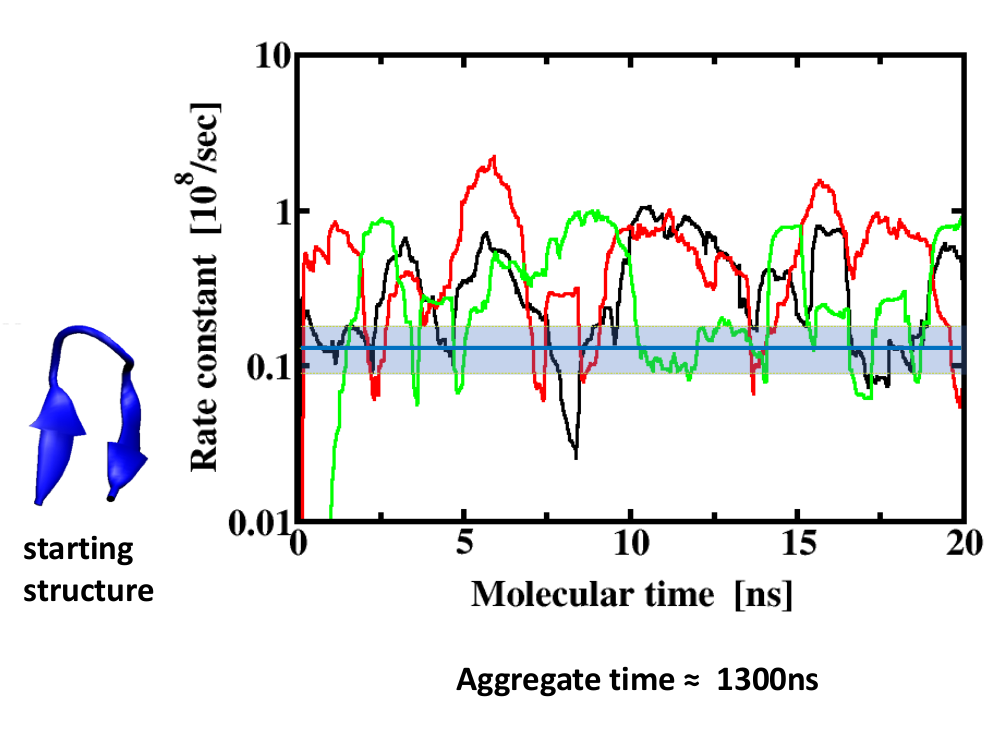
\includegraphics[width=\linewidth]{Figure10.png}
\caption{Estimating the unfolding rate constant of chignolin. 
The 1 ns window-averaged unfolding rate constant is shown in a semi-logarithmic plot for three independent WE simulations (black, red, and green) that were started from the same folded starting structure (see lower left). 
The corresponding unfolding rate constant from the brute force simulation is indicated by the horizontal blue line and its confidence interval by the shaded region. 
The molecular time is the time elapsed, N\textsubscript{$\tau$} where N is the number of WE iterations that each have a length of $\tau$. 
The aggregate simulation time was on average, \textasciitilde 1.3 $\mu$s for each simulation.}
\label{fig:chig-flux}
\end{figure}
%%%%%%%%

\textbf{Figure \ref{fig:chig-flux-3}} shows the evolution of the average folding rate constant for chignolin as a function of molecular time for three independent WE simulations. 
Compared with unfolding simulations, the folding simulations require much longer to reach a converged average rate constant that is in rough agreement with that from the brute force simulations; we note that the average rate constant is dominated by the largest flux. 
In addition, the folding rate constant exhibits significantly larger fluctuations, even after the apparent transient period of the first \textasciitilde 100 ns, indicating that the chosen bins are less suited for the folding process. 
During the folding process, distinct hydrogen bonds must be formed between the neighboring anti-parallel strands, and possibly in a specific order, to eventually reach an RMSD < 0.5 \AA. 
In contrast, the unfolding process results in faster convergence of the corresponding rate constant and likely involves the simultaneous breaking of hydrogen bonds in order to reach an RMSD > 4 \AA.

%%%Fig 11%%%
\begin{figure}
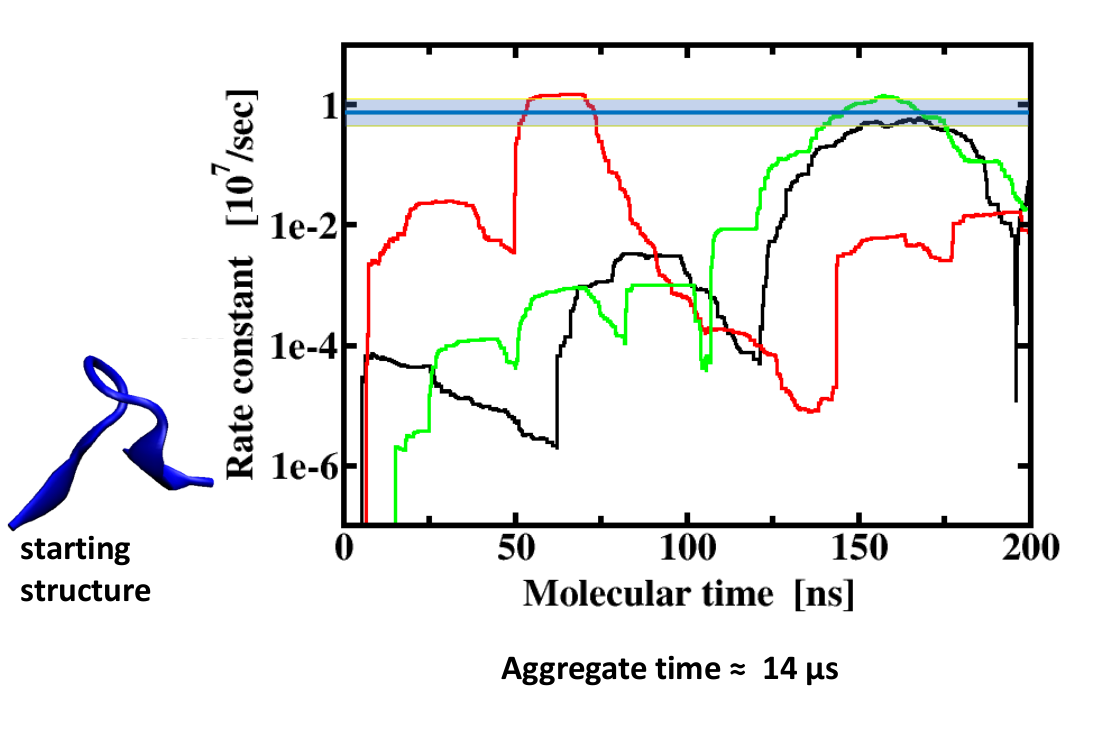
\includegraphics[width=\linewidth]{Figure11.png}
\caption{Estimating the folding rate constant of chignolin. 
The 20-ns window-averaged folding rate constant is shown in a semi-logarithmic plot for three independent WESTPA simulations (black, red, and green profiles) with the same unfolded starting structure (see lower left). 
Note the significantly longer molecular and aggregate simulation times for each simulation to obtain converged rate constants of folding compared to unfolding (see \textbf{Figure \ref{fig:chig-flux}}). 
The corresponding rate constant from the brute force simulation is indicated by the horizontal blue line and its confidence interval by the shaded region.}
\label{fig:chig-flux-3}
\end{figure}
%%%%%%%%

The resulting WE simulations consist of multiple continuous unfolding or folding pathways that may cover different regions of configurational space at any given time. 
To select for particular pathways (trajectories), we can run the following: 
\begin{verbatim}
  $ python get_target_trajs.py  1  10000
\end{verbatim}
The command-line arguments indicate the first and last iteration number to be considered. 
The output file \verb|target_trajs.dat| has two columns: one with the iteration number and one with the segment number of the trajectory that has reached the target state at that iteration. 
Thus, the number of rows indicates the total number of generated events. 
The iteration and segment numbers can be used by \verb|w_trace| to obtain the full path of a particular folding or unfolding event (see \textbf{Section \ref{tut:basic-nacl-monitoring}}).

\subsubsection{Conclusion}

In this tutorial, you have learned how to apply the WE strategy to simulate a protein folding process under steady state conditions. 
The recycling of trajectories at a target state allows the generation of a non-equilibrium steady state, to which the trajectory ensemble converges faster compared to an equilibrium ensemble of trajectories. 
Such steady states trajectories enable  the direct computation of rate constants as described in this tutorial.
\vspace{-0.125cm}

\begin{comment}
\subsection{Advanced Tutorial: K\textsuperscript{+}/18-Crown-6 Ether Dissociation with the WExplore Plugin}
\label{tut:crown-wexplore}

\subsubsection{Introduction}

For many biomolecular systems, it can be difficult to capture all of the slow motions in one or two collective variables. 
This can hinder sampling of the events of interest. 
The WExplore algorithm was developed to perform WE sampling in a many-dimensional space by using a hierarchical binning scheme of Voronoi polyhedra. 
This allows a user to broadly explore the dynamics of their system of interest along many dimensions, starting from only a single initial structure.

The key quantity to enable this is a distance metric: a way of measuring the distance between two trajectories at a given point in time. 
In order to assign a given trajectory, $X$, to a region, this metric is used to calculate the distance from $X$ to a set of “images” that define the Voronoi polyhedra. 
The trajectory $X$ is then assigned to the region whose image has the smallest such distance. 
To efficiently assign trajectories to regions in a high-dimensional space, a hierarchy of regions is employed: a small set of very large regions tile the full space, each of which are tiled by a set of smaller regions, which are themselves tiled by smaller regions, and so on. 
The WESTPA-WExplore plugin defines the hierarchical regions on-the-fly; assigns trajectories to regions; and balances trajectories between the hierarchical regions. 
The user only needs to define the distance metric appropriate for their system and set a few parameters of the algorithm.

\textbf{Learning Objectives.} This tutorial covers the installation and use of the WESTPA-WExplore plugin for a simple system: the dissociation of a K\textsuperscript{+} ion from 18-crown-6 ether.

Specific learning objectives include:
\begin{enumerate}
\item How to install and use the WExplore-WESTPA plugin
\item How to define and implement a distance metric for use in WExplore simulation
\item Determining appropriate values for WExplore-specific parameters for a system of interest
\item Analyzing simulations by inspecting properties of the Voronoi “images” 
\end{enumerate}

Users with some WESTPA experience should be able to successfully apply WExplore to their system of interest using their own customized distance metric.

\subsubsection{Prerequisites}

Users should have completed the WESTPA tutorials above on Na\textsuperscript{+}/Cl\textsuperscript{-} and the p53 peptide. 
Users should have an understanding of the WExplore algorithm: how the region hierarchy is defined; how it progressively discovers regions; and how the hierarchical balancing algorithm works. 
Details of the algorithm can be found in previous work \citep{dickson_wexplore_2014}. 

\textbf{Computational Requirements.} This tutorial requires 500 MB disk space. 
This simulation takes \textasciitilde 1.5 hours of wall clock time to complete (50 iterations) using 8 threads of a 4 GHz Intel Core i7 processor.  
This tutorial uses Gromacs 2016.2 for dynamics propagation and progress coordinate calculations (\url{http://www.gromacs.org/}).  
Gromacs is available free of charge.

\subsubsection{Installation and Configuration of the WESTPA-WExplore Plugin}

It is necessary to install some other Python packages that you might not need for standard WESTPA simulations. 
We recommend using an Anaconda environment and installing the packages as follows:

\verb|$ conda create -n WESTPA-WExplore westpa scipy|

\verb|pandas networkx|

\verb|$ conda activate WESTPA-WExplore|

Note that if you are running your WESTPA simulations on remote nodes, you would have to include the \verb|conda activate| command in your \verb|env.sh| file. 
To install the plugin, clone the WESTPA-WExplore repository to a location on your computer:  

\verb|$ git clone https://github.com/ADicksonLab/|

\verb|WESTPA-WExplore.git|

This will copy files to your machine, located in the \verb|WESTPA-WExplore/| directory. 
Change to this directory and install the plugin as follows:

\verb|$ cd WESTPA-WExplore/|

\verb|$ python setup.py install|

To test this, go to another directory, and type:

\verb|$ python -c 'import westpa_wexplore'|

If this runs without an import error, then you are ready to proceed to the next step! 

\subsubsection{Preparing the Simulation}

\textbf{The System.} This tutorial will use a simple ligand-binding test system: the dissociation of a K\textsuperscript{+} ion from the 18-crown-6 ether molecule (\textbf{Figure \ref{fig:crown}}), as studied previously \citep{Zwier2011}. 
The goal is to efficiently sample the dissociation of the complex. 
This is reminiscent of applications of WExplore to more difficult ligand dissociation problems, such as the unbinding of the TPPU ligand from soluble epoxide hydrolase, a process with a mean first passage time of 11 minutes \citep{Lotz2018}.

%%%Fig 12%%%
\begin{figure}
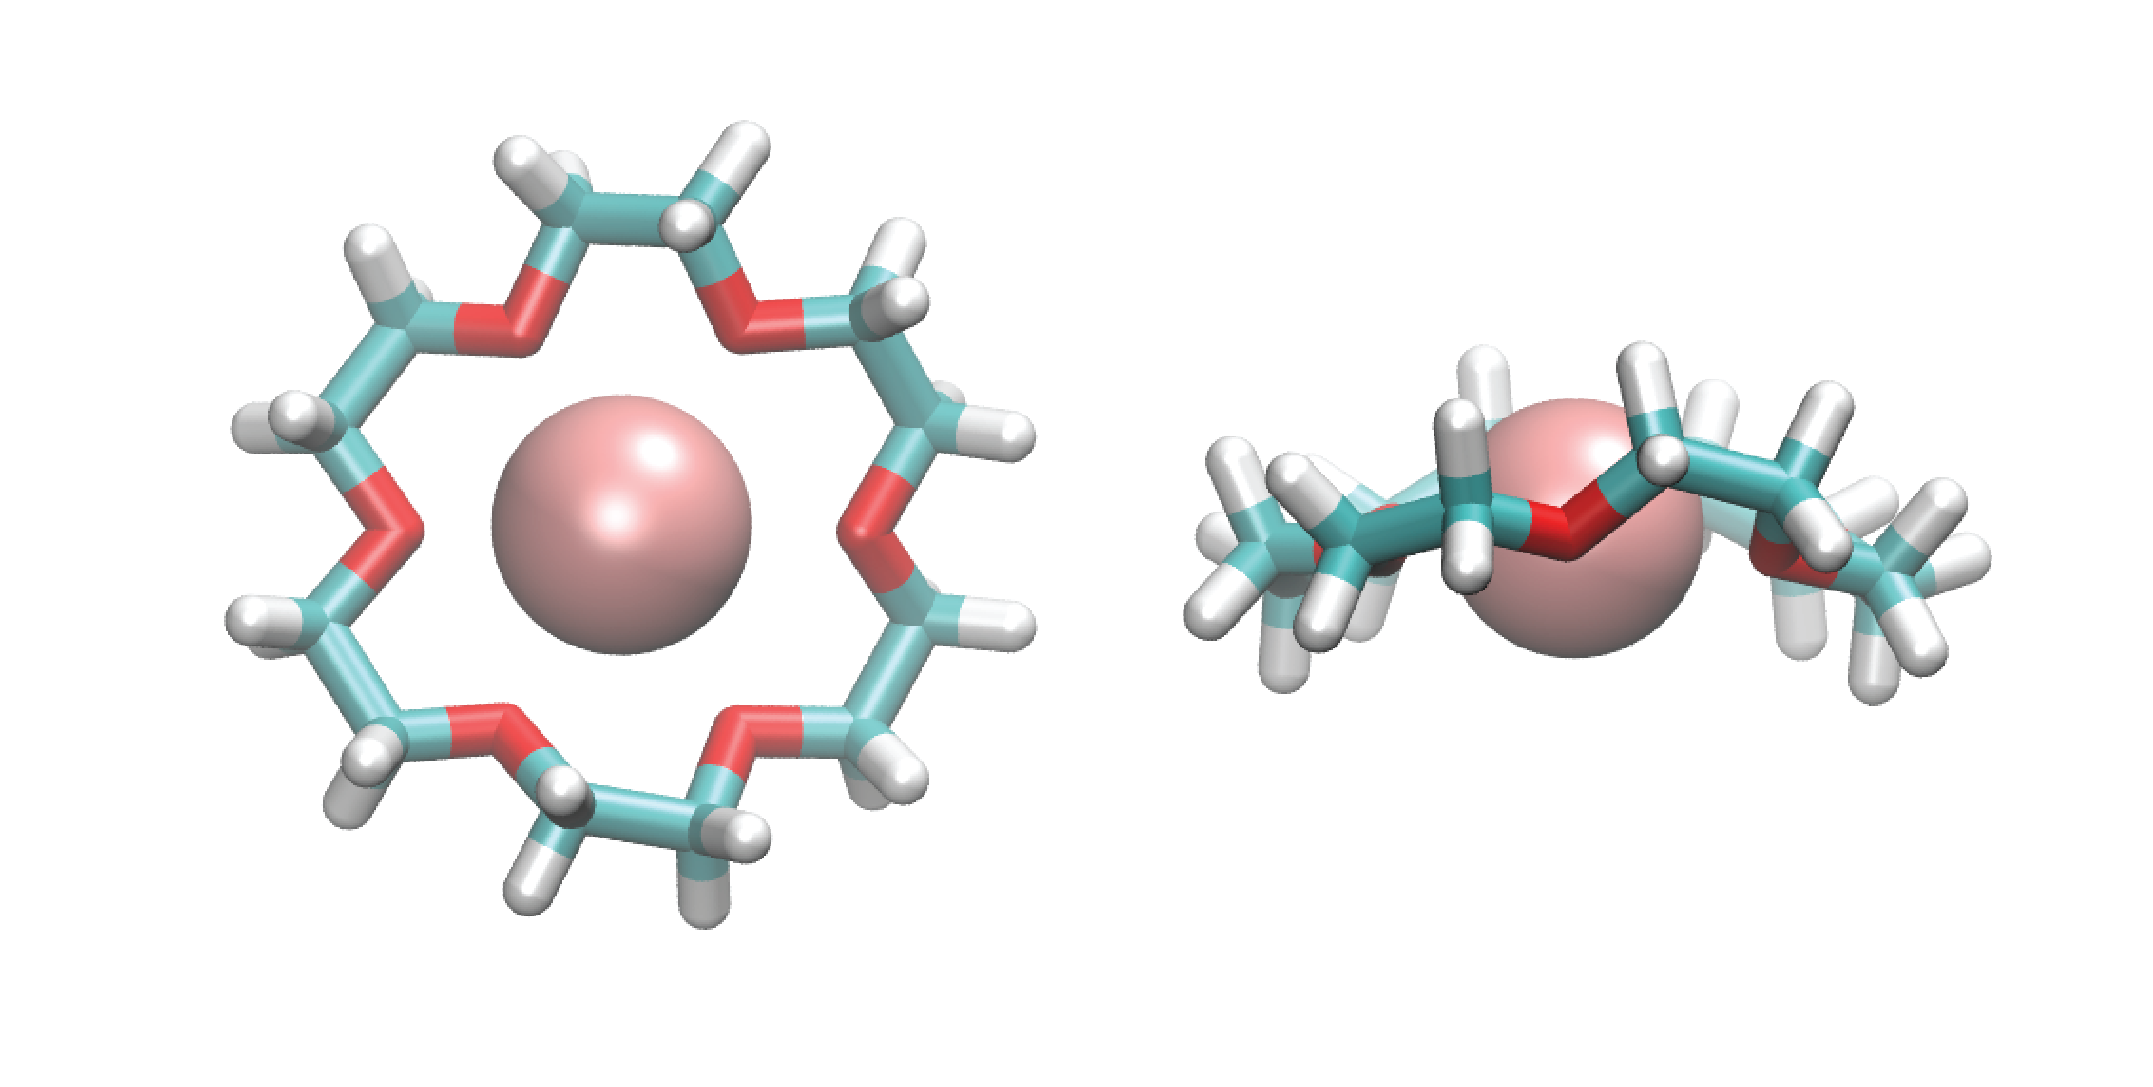
\includegraphics[width=\linewidth]{Figure12.png}
\caption{The K\textsuperscript{+}/18-Crown-6 ether system. 
The K\textsuperscript{+} ion is shown as a pink sphere. Left: top view. Right: side view.}
\label{fig:crown}
\end{figure}
%%%%%%%%

\textbf{Distance Metric.} Here we will use a common distance metric for ligand release processes: the root mean squared distance of the ligand atoms after alignment to the host binding site \citep{Dickson2017,Dixon2018,Dickson2018}.
This captures ligand translation with respect to the binding site, and (for systems with more complicated ligands) captures ligand rotation as well as internal degrees of freedom. 
The information needed to calculate these distances is the x, y and z positions of the ligand atoms after alignment to the host molecule. 
The first step to assign a walker to a region, then, is to extract this data from the simulation. 
This is done by a familiar script: \verb|get_pcoord.sh|.

The \verb|get_pcoord.sh| script included in the tutorial repository uses a series of bash commands to align a crown ether molecule to a reference structure (named \verb|bound_state.tpr|), and then extracts only the lines that contain the ligand atoms, saving them in the file indicated by the \verb|WEST_PCOORD_RETURN| environment variable. 
This data is then processed by the \verb|pcoord_loader| function in the \verb|system.py| file, where the x, y and z data are collected from columns 5, 6 and 7 of the PDB-formatted file. 

This pipeline is rather crude, but effective. 
Note that any set of commands that can extract the output you need (typically, atomic positions) from your simulation output files will do, but it is necessary that changes that you make to \verb|get_pcoord.sh| (which writes to \verb|WEST_PCOORD_RETURN|) are compatible with any changes you make to \verb|pcoord_loader| (which reads from \verb|WEST_PCOORD_RETURN|). 
For instance, one could avoid PDB files all together, and load final structures into the \verb|pcoord_loader| using the Python interface of Amber or Gromacs.

The next step is to define a function that returns the distance between two pcoord vectors. 
This is typically a Euclidean distance, but can be defined in an arbitrary fashion. 
It need not be differentiable, or even continuous, to be effective in a WExplore simulation. 
The distance function is defined by \verb|eucl_dist| in \verb|system.py| and is passed as an argument to the \verb|WExploreBinMapper| function upon initialization of a system object.

\textbf{Setting parameters.} The set of WExplore-specific parameters were discussed above in Section 3.1. 
Most of these are set in the \verb|system.py| file. The sizes of the hierarchical Voronoi polyhedra are set using a list, passed to the \verb|d_cut| argument of the \verb|WExploreBinMapper| function. 
This list should go from largest to smallest, where the number of elements is the same as the number of levels to the hierarchy. 
Similarly, the branching factor is set by a list that is passed to the \verb|n_regions| argument of \verb|WExploreBinMapper|. 
The number of total trajectories is set by the \verb|max_replicas| attribute of the system.

\textbf{Choosing an Initial State.} It is also necessary, upon initializing the system object in \verb|system.py|, to define the initial “image” that corresponds to the first structure used in the simulation. 
This is done in lines 35-37 of the \verb|initialize| function in \verb|system.py| and should be changed as necessary for a given system. 
The initial PDB file containing the aligned K\textsuperscript{+} coordinates was prepared from the basis state 0 (in bstates/0) using Gromacs in the \verb|init.sh| script. 
As described in \verb|BASIS_STATES.single|, we are initializing all trajectories from a single starting structure (“bound\_0”) that has probability = 1.

\textbf{Other parameters.} Other details of simulation parameters are given in the \verb|md.mdp| file. 
For instance, the dynamics timestep (0.002 ps), the number of steps per cycle (1000) and the output frequency for coordinates, velocities and forces (100, 100 and 0, respectively) are specified here. 
Note that here we are outputting our coordinates 11 times per cycle (1000 / 100, plus one extra for the endpoint). 
This must be consistent with the parameter \verb|pcoord_len| in \verb|system.py|, which is also set to 11 in our case.

\textbf{Preparing the Simulation Environment.} As discussed previously, make sure to modify the env.sh file to reflect the installation locations of WESTPA, Gromacs, etc. on your machine. 
Additionally, add the location of the WESTPA-WExplore package to your \verb|WEST_PYTHONPATH|, e.g.:

\verb|export WEST_PYTHONPATH=/your/installation/|

\verb|location/WESTPA-WExplore/westpa_wexplore:|

\verb|$WEST_PYTHONPATH|

\subsubsection{Running the Simulation}

First we need to initialize the simulation:

\verb|$ ./init.sh|

And then we can run a job. 
This can be submitted to a cluster (we will not go over that here), or run locally, as follows:

\verb|$ ./run.sh --parallel --n-workers 8|

This is a good time to break for lunch. 
In our hands, this will take about 90 minutes on a 4 GHz Intel Core i7 processor.

\subsubsection{Analyzing the WExplore Simulations}

Aside from the way that resampling is implemented, WExplore simulations can be treated just like other WE simulations in terms of analysis. 
All of the techniques discussed above regarding the definition of observables and plotting of probability distributions can be used for WExplore simulations as well. 
Here we will briefly go over how to analyze simulation properties that are unique to WExplore. 
Specifically, the location of the “images” used to define the Voronoi polyhedra.

Firstly, during run time it can be helpful to keep an eye on the number of regions defined so far at each level of the hierarchy. 
A brief report is written, each cycle, in \verb|west.log|:

\verb|--wexplore-stats--------------------|

\verb|wallclock time: 0.221 s|

\verb|Level 0: 10 cells (10 max)|

\verb|Level 1: 69 cells (100 max)|

\verb|Level 2: 193 cells (1000 max)|

\verb|------------------------------------|

\verb|Iteration wallclock: 0:01:41.246056,|

\verb|cputime: 0:12:40.570392|

This is taken from the end of our simulation, where we have defined 10 regions at the largest level of the hierarchy (here, they are at least 5 \AA{} apart), 69 total regions at the medium level (some of which are under the first large region, some under the second, and so on), and 193 total regions at the smallest level. 
It is completely fine if these numbers do not approach their maximum values. 
In contrast, if regions are defined too quickly – especially at the smallest level – then this is a sign that they are too small.  
The log file also displays the wall clock time for the WExplore resampler (0.221 s), which is negligible compared with the total wall clock for the cycle (1 minute, 41 s), as is typical.

The details about the WExplore regions are stored in \verb|west.h5|, along with the positions and progress coordinates. 
The included Python script (\verb|WExplore_analysis.py|) shows how the coordinates of the images can be accessed from the \verb|west.h5| file and analyzed using Python tools like \verb|numpy| and \verb|MDTraj| \citep{mdt2015}.

\subsubsection{Conclusion}

Users should now have everything they need to use the WExplore resampling algorithm on their own system of interest.  
WExplore is a powerful way to generate heterogeneous sampling on energy landscapes that are both rough and high-dimensional. 
The ability to write your own distance metric using tools in Python opens up many possibilities. 
For example, a number of dimension reduction tools in sklearn could be easily imported and used to automatically identify a space of collective variables.  

\end{comment}

\subsection{Analysis Tutorials}
\label{tut:analysis-adv}

In this tutorial, we will go over how to calculate progress coordinates using external analysis suites, automate analysis of a WE simulation using the WESTPA \verb|w_ipa| tool and visualize the evolution of WE datasets with time. 
We focus on the p53 peptide system described above in the \textbf{Intermediate Tutorial \ref{tut:p53-int}} in which the progress coordinate is the C\textsubscript{$\alpha$} RMSD of the peptide from its folded, $\alpha$-helical conformation.

\subsubsection{Calculating Progress Coordinates Using External Analysis Suites}

\textbf{Introduction.} Here we will demonstrate how to write scripts for calculating custom progress coordinates for WESTPA simulations using the external analysis suites MDAnalysis and MDTraj \citep{mda2011,mda2016,mdt2015}. 
A prerequisite to this tutorial is completion of the \textbf{Basic Tutorial \ref{tut:nacl-basic}}. 
You will also need to install the MDAnalysis or MDTraj analysis suites. 
Other required files are provided on GitHub.

\textbf{Learning Objectives.} The specific learning objective of this tutorial is to calculate progress coordinates using an external analysis suite (MDAnalysis or MDTraj). 

\textbf{Explanation of Files and Scripts.} The master configuration file for the simulation, \verb|west.cfg|, specifies the dimensionality of the progress coordinate (\verb|pcoord_ndim|), as well as how many progress coordinate data points should be returned from each segment (\verb|pcoord_len|) (it specifies many other things but these are of primary interest for this tutorial as they specify the shape of the progress coordinate).

The script \verb|rmsd.py| is responsible for using MDTraj or MDAnalysis to calculate the RMSD values during the simulation. 
Read the comments in the script to understand its setup for each package (there is a unique version for both).

Two scripts are responsible for calling \verb|rmsd.py| at different points in the simulation (both found in \verb|westpa_scripts/|):
\begin{itemize}
\item \verb|get_pcoord.sh| calculates the progress coordinate during the initialization of the system. 
Because dynamics have not been run yet, WESTPA only needs a single point progress coordinate, rather than an array. 
This difference is controlled by the FORM argument, explained in the \verb|rmsd.py| script.
\item \verb|runseg.sh| calculates the progress coordinate during dynamics propagation. 
It passes each segment's trajectory file as input to the custom progress coordinate loader, \verb|rmsd.py|.
\end{itemize}

There are slight differences in these files for the MDAnalysis and MDTraj setups, explained in the comments of each script.

\noindent \textbf{Files in amber\_config/ directory:}
\begin{itemize} 
\item \verb|P53.MDM2.prmtop| - The topology file.
\item \verb|md.in| - The input file which specifies conditions for dynamics propagation.
\end{itemize}

The other files needed for the simulation are found in the bstates folder, and are explained in the MDAnalysis/MDTraj specific sections below.

\textbf{Running the Simulation.} Before running the simulation, you may want to change the binning scheme, the number of iterations, or other parameters, which can be found in \verb|west.cfg|.

\noindent To run the simulation, only two scripts must be executed. 

\noindent To initialize the system:

\begin{verbatim}
  $ ./init.sh
\end{verbatim}

\noindent To run the simulation in the background:
\begin{verbatim}
  $ ./run.sh &
\end{verbatim}

\noindent To monitor the progress of the simulation:
\begin{verbatim}
  $ tail -f west.log
\end{verbatim}

The rest of the tutorial is specific to the software package used. 
See below for specifics involving the MDAnalysis and MDTraj analysis suites.

\textbf{Using the MDAnalysis Analysis Suite}

Files in \verb|bstates/| directory:
\begin{itemize}
\item \verb|P53.MDM2.ncrst| - Used as initial crystal structure to compare to the trajectory when calculating the RMSD and to start new trajectories in \verb|runseg.sh|.
\item \verb|bstates.txt| - specify restart file \verb|P53.MDM2.ncrst|.
\end{itemize}

\textbf{Using the MDTraj Analysis Suite}

Files in \verb|bstates/| directory:
\begin{itemize}
\item \verb|P53.MDM2.nc| - because MDTraj does not support restart files, this file is used in \verb|get_pcoord.sh| to calculate the initial progress coordinate. 
It is also used by \verb|runseg.sh| as an initial crystal structure to compare to the trajectory when calculating the RMSD.
\item \verb|P53.MDM2.ncrst| - Used to start new trajectories in \verb|runseg.sh|.
\item \verb|bstates.txt| - specify restart file \verb|P53.MDM2.ncrst|.
\end{itemize}

\textbf{Conclusion.} You have learned in this tutorial the basic structure of a Python script to calculate progress coordinates for WESTPA using the MDAnalysis and MDTraj analysis suites. 
There are two scripts run by WESTPA which call \verb|pcoord_loader.py|, triggering the calculation of progress coordinates. 
The bash script, \verb|get_pcoord.sh|, triggers the calculation of only a single progress coordinate, while \verb|runseg.sh| triggers the calculation of the progress coordinate at multiple points in a trajectory, as defined in \verb|west.cfg|. 
It is important to include the last line of the Python scripts, setting \verb|segment.pcoord| equal to the progress coordinate array, so that the progress coordinate may be used to further the simulation.

\subsubsection{The w\textunderscore ipa Analysis Tool}
\label{tut:analysis_adv_w_ipa}

\textbf{Introduction.} The \verb|w_ipa| analysis tool is designed to facilitate analysis of WESTPA simulation datasets through a single interface (Jupyter Notebooks or the command line). 
In particular, \verb|w_ipa| automates analysis routines, ensures data consistency through the use of automatically updated “analysis schemes”, enables a user to easily view a particular dataset or trajectory segment in the H5 file, and monitors the progress of the simulation (e.g. trajectory weights, progress coordinates, and other properties of interest).  

Learning Objectives. The specific learning objectives of this tutorial are to use the \verb|w_ipa| analysis tool to:
\begin{enumerate} 
\item Calculate rate constants
\item Trace and analyze trajectory segments (weight, pcoord, auxdata)
\item Plot datasets
\end{enumerate}

\textbf{Setting Up.}  Using \verb|w_ipa| is straightforward. 
The \verb|west.cfg| file, which specifies most of the simulation parameters, also specifies the analysis parameters under the \verb|Analysis| heading.

The general format of the analysis section can be seen in the included \verb|west.cfg| file. 
More detailed examples are available in the \textbf{Basic and Intermediate Tutorials} (\textbf{Sections \ref{tut:nacl-basic}-\ref{tut:chig-int}}).

In order to run \verb|w_ipa|, there must be at least a single analysis scheme specified. 
This scheme does not have to consist of the bins and/or state definitions used during the simulation. 
Less physically relevant schemes may be employed. 
Any changes made to analysis schemes in the \verb|west.cfg| file will be actualized the next time \verb|w_ipa| is run. 
The user is therefore guaranteed to never wonder whether the analysis files are up to date. 

The \verb|assign.h5|, \verb|reweight.h5|, and \verb|direct.h5| files are stored under \verb|ANALYSIS/SCHEME_NAME|.
The optional arguments that can be passed to \verb|w_assign|, \verb|w_direct|, and \verb|w_reweight| can be specified by creating a section with the tool name and using the value pairs argument. 

\textbf{The Interface}. To run \verb|w_ipa| from the command line, enter the command \verb|w_ipa| after having sourced \verb|westpa.sh| (if not already sourced). 
To run \verb|w_ipa| in a Jupyter notebook enter the command \verb|w_jupyter| from the command line. 
When you create a new Jupyter notebook, there are some basic Python commands that must be executed:

\begin{verbatim}
  import w_ipa
  w = w_ipa.WIPI()
  # At startup, it will load or run the analysis
   schemes specified in the configuration file
   (typically west.cfg)
  w.main()
  w.interface = 'matplotlib’
\end{verbatim}

The Python kernel must be launched with the use of \verb|w_jupyter|, or otherwise, the \verb|$PYTHON_PATH| variable must be set to include the WESTPA directories. 
The command \verb|w_env|, which ships with WESTPA, is responsible for setting environment variables and can be used with the Jupyter notebook command to ensure \verb|w_ipa| is importable.

All commands are applicable from both the command line and Jupyter notebook interface; if plotting functions are called from the command line, the plot will appear within the console (it can be configured to use matplotlib if desired; this requires an active, available X session).

All of the variables are now accessible from the \verb|w| object.

\textbf{Changing Schemes and Accessing Datasets.} A typical analysis routine begins by selecting an appropriate analysis scheme that may consist of multiple state definitions, averaging options, or reweighting parameters that are appropriate for the simulation. 
Most of the datasets are presented from the current, “active” state, although access to other datasets is conveniently available. 
All numerical datasets are given as NumPy arrays, allowing for easy analysis of data.

To see what schemes are available, run the following command:

\begin{verbatim}
  $ w.list_schemes
\end{verbatim}

To change schemes, you may set the \verb|w.scheme| variable to a string or integer value (corresponding to the index of the scheme). 
For instance, suppose you have the following two schemes: “\verb|EXAMPLE|”, and “\verb|ALTERNATE|”, and the current scheme is "\verb|EXAMPLE|". 
To access the properties of the current iteration in the current scheme (explained in more detail below), you would type the following:
\begin{verbatim}
  $ w.current
\end{verbatim}

However, to access the alternate scheme, you would run the following command:
\begin{verbatim}
  $ w.schemes.ALTERNATE.current
\end{verbatim}

Where “\verb|ALTERNATE|” corresponds to the scheme name written in the \verb|west.cfg| file.

The \verb|w_ipa| tool works by presenting an iteration and all its data as a single object. Each iteration object contains numerous datasets and helper functions designed to ease analysis. 
After loading, \verb|w_ipa| defaults to the final iteration. 
You can change the iteration by using the following command: 
\begin{verbatim}
  $ w.iteration = 39
\end{verbatim}

At any time, we have three iteration objects available in the object \verb|w|: current, past, future. 
The past and future datasets are keyed to the parents and children of the segments in the current dataset. 
For instance, if you are analyzing segment 200 in the current iteration and wish to analyze the parent segment it came from, you could access the two datasets using the following iteration objects:

\begin{verbatim}
  $ w.current[200]
  $ w.past[200]
\end{verbatim}

Even though it is very unlikely that the actual segment ID of the parent of segment 200 is 200, it is mapped correctly to enable convenient analysis. 
To obtain the actual segment ID, just run:

\begin{verbatim}
  $ w.past[200].seg_id
\end{verbatim}
OR
\begin{verbatim}
  w.past[200][‘seg_id’]
\end{verbatim}

As indicated above, objects in \verb|w_ipa| can be called either as Python dictionaries or as attributes on the object. 
These can be listed by calling the print method on the parent object. 
In addition, as \verb|w_ipa| is using iPython under the hood, tab completion works as when using the command-line interface (CLI).

To access the main datasets of interest, \verb|pcoord| and \verb|auxdata|, type the following: 
\begin{verbatim}
  $ w.current.pcoord
  $ w.current.auxdata
\end{verbatim}

These commands will output the full datasets, which can be useful for calculating properties on all trajectory segments at once. 
But what if we are only interested in looking at the properties of particular segments?

You could manually find a segment of interest, but \verb|w_ipa| includes a few convenient properties that return certain segments. 
In particular, \verb|w.current| provides the following:

\begin{verbatim}
  maxweight
  minweight
  successful_trajectories
\end{verbatim}

The \verb|maxweight| and \verb|minweight| properties return objects which contain data about the segments that carry the highest and lowest weights in the current iteration, respectively. 
The \verb|successful_trajectories| property returns the IDs of the segments that successfully transitioned between states  (the states are defined in your \verb|west.cfg|). 
Calling these functions on an iteration object yields all datasets pertaining to the segment with the desired property. 
In this WE simulation, each trajectory contains 101 timepoints. 
Therefore, the \verb|maxweight| segment (seg\_id 177) in iteration 49 has (101,2) pcoord values, 101 auxdata values, and it can switch bins and states 101 times. 
You can see this by running \verb|w.current.maxweight|.
 
The auxdata dataset is unique in that the simulations can contain any number of auxiliary datasets with any unique name. 
Here, they are returned as a dictionary where the key is the dataset name defined in \verb|west.cfg| and the value is a NumPy array containing the actual dataset.

Segment 177 above was in state 1 during the entire iteration. 
But what is state 1? 
It is defined in \verb|west.cfg|, but we do not have to go back to \verb|west.cfg| to look it up. 
Simply run:
\begin{verbatim}
  $ w.state_labels
\end{verbatim}

It is also in bin 0 the entire time (note that these are the bins defined in \verb|west.cfg| for this analysis scheme and not the bins used in the simulation). 
What is the pcoord value of that bin? Run:

\begin{verbatim}
  $ w.bin_labels
\end{verbatim}

To track the immediate parent and children of a segment, we can use \verb|w.past| and \verb|w.future|. 
These iteration objects are similar to \verb|w.current|, but keyed to give information about the segments in \verb|w.current|. 
For instance, to look up the weight of segment 177’s parent, run the following:

\begin{verbatim}
  $ w.past[177].weights
\end{verbatim}

Likewise, to see whether the same segment had any children, run:

\begin{verbatim}
  $ w.future[177]
\end{verbatim}


Segments always have a past, but do not always have a future. 
They may also produce multiple children, so the values returned by \verb|w.future[seg_id]| are usually more complicated. 
Rather than being given the datasets directly, \verb|w.future| returns a list of the datasets.

To determine the properties of a complete trajectory (that is, the string of segments going back to the first iteration), \verb|w_ipa| includes a fast trace function. 
To trace segment 177 in iteration 39 (current iteration), run the following:
\begin{verbatim}
  $ s = w.trace(177)
\end{verbatim}

It returns an object similar to \verb|w.current[177]|, except that it also contains all historical information. 
The \verb|auxdata|, \verb|bins|, \verb|pcoord|, and \verb|states| datasets are all going to be very large; their shape should be the product of the number of timepoints per iteration and the trajectory length. 
As we are at iteration 39, and have 101 time points per $\tau$ value, we should have 3939 values in each dataset! 

\textbf{Plotting.} Rather than visually inspecting each value, let us just plot it. 
Run the following:
\begin{verbatim}
    $ clear
    $ s.weights.plot()
    $ clear
    $ s.pcoord.plot()
    $ clear
\end{verbatim}


Many datasets, such as \verb|weight|, default to a logscale; others, such as \verb|pcoord|, use a linear scale. 
By default, the 0th dimension of \verb|pcoord| is plotted. 
When the plotting function is called via the CLI, a rough estimate of how the trajectory’s pcoord has evolved is plotted in the terminal.

The \verb|w.current| iteration object contains information about the rate constants that were calculated in the active analysis scheme. 
To view an array containing the rate constants along with the upper and lower confidence intervals, run the following (do not forget about tab completion): 
\begin{verbatim}
  $ w.current.direct.rate_evolution
\end{verbatim}
OR
\begin{verbatim}
  $ w.current.rate_evolution.direct
\end{verbatim}

\noindent To view a plot of their evolution, run the following:
\begin{verbatim}
  $ w.current.direct.rate_evolution.plot()
\end{verbatim}

The \verb|w_ipa| tool displays the upper and lower confidence intervals on the plot as well. 

\subsubsection{Visualization of WE Datasets}
\label{tut:analysis_adv_visualization}

In addition to generating probability distributions as a function of the progress coordinate (or other observables of interest), it can be helpful to examine movies of how the distributions evolve with time. 
Such movies can be used to determine the optimal number of trajectories per bin in a particular region of the progress coordinate by tracking how the probability distribution evolves with the number of trajectories that region. 

\textbf{Learning Objectives.} The specific learning objectives of this tutorial are:
\begin{enumerate}
\item Create a movie of how a probability distribution evolves with time.
\item Trace representative trajectories over this probability distribution.
\end{enumerate}

Here, we will create a movie of how a two-dimensional probability distribution (\textbf{Figure \ref{fig:landscape-traj}}) evolves with time. 
This movie-making feature is currently carried out using a bash script (\verb|pdist_evol.sh|) and will eventually be added to the WESTPA \verb|plothist| tool. 

%%%Fig 12%%%
\begin{figure}[t]
\centering
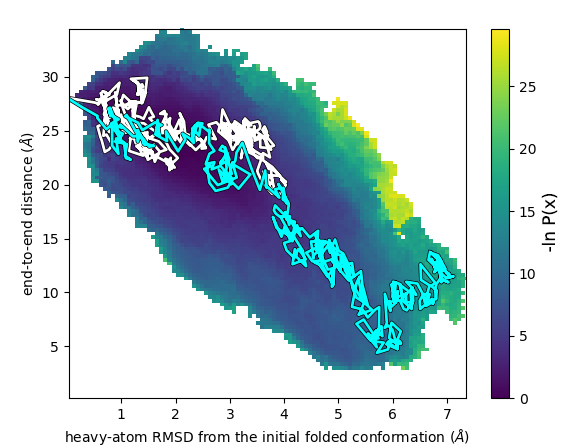
\includegraphics[width=\linewidth]{figures/Figure13-2.png}
\caption{Two-dimensional probability distribution as a function of the progress coordinate. 
Two representative, continuous trajectories that originate from distinct initial states are traced in cyan and white, respectively.}
\label{fig:landscape-traj}
\end{figure}
%%%%%%%%

The bash script involves the following three steps: (1) run the \verb|w_pdist| tool on the \verb|west.h5| file to generate probability distributions in a specified folder that will also contain the eventual movie of how the distributions evolve with time, (2) generate a plot of a two-dimensional probability distribution for each iteration as a cumulative moving average from iteration 1 to 40 and (3) create the movie from the 40 generated frames of the probability distributions. 
The most important part of this script is the \verb|--postprocess-function| option of \verb|plothist| that is defined in \verb|postprocess.py|. 
This function requires a basic knowledge of Python and \verb|matplotlib|, and can be used to modify features of the plot (e.g. adjustment of axis labels, tick marks, titles, and lines) via the \verb|matplotlib| interface. 
In addition, external files from various analyses can be uploaded and overlaid on the plot as demonstrated in this example. 

Here, we will select two trajectories from the last WE iteration and overlay their pathways on the probability distribution of the overall simulation as a function of progress coordinate. 
First, we will use the \verb|trace_walker| function to determine the segment number of the selected trajectories in each WE iteration going all the way back to the corresponding conformation of the initial state ensemble. 
This process of tracing can also be accomplished by using WESTPA tools \verb|w_ipa| and \verb|w_trace|. 
After the segment numbers are obtained, the \verb|get_pcoords| function loads in 10 progress coordinate values per iteration for the trajectories. 
Finally, a movie-making tool (here, we use \verb|mencoder|) creates a movie from the 40 frames of probability distributions.  %MRS: th is a bunch of the old stuff!

%\section{Advanced Tutorials}

\subsection{Creating “Binless” Resampling Schemes: Na\textsuperscript{+}/Cl\textsuperscript{-} Association Simulations}

%%% For anyone trying to edit the source LaTeX code, the ~ are here to help space out the text so short words like 'Basic' doesn't get spread out across two lines. Sorry, there is no better solution. 

\subsubsection{Introduction}
The non-linearity of certain progress coordinates (e.g., those identified by machine learning tools) requires the creation of “binless” rather than binned resampling schemes for rare-event sampling. 
In addition, binless schemes can be useful in grouping trajectories by a feature of interest for resampling. 
For example,~ trajectories~ could~ be~ grouped~ by history~ (sharing the same parent structure) to improve the diversity of trajectories that successfully reach the target state, or by a simple k-means clustering. 
This tutorial builds upon the Basic WESTPA Tutorial (Na\textsuperscript{+}/Cl\textsuperscript{-} association simulations) \citep{bogetti_suite_2019} by introducing users to running and analyzing a WESTPA simulation that employs “binless” resampling schemes.
~ This~ tutorial~ is a prerequisite for \textbf{Advanced Tutorials 3.2-3.4}. 

\textbf{Learning Objectives.} This tutorial introduces users to the generalized resampler module in the WESTPA 2.0 software package that allows for the creation of either binned or binless resampling schemes.

The tutorial also instructs users on how to initiate a WE simulation from multiple representative conformations of the starting state and how to apply two key post-simulation analysis tools. 
Specific learning objectives are:
\begin{enumerate}
    \item How to create a binless scheme for splitting and merging trajectories based on k-means clustering using the \verb|BinlessMapper| resampler module;
    \item How to initiate a WE simulation from multiple starting conformations;
    \item How to combine multiple WE simulations for analysis using the \verb|w_multi_west| tool;
    \item How to perform post-simulation analysis using the \verb|w_crawl| tool.
\end{enumerate}

\subsubsection{Prerequisites}

\textbf{Computational Requirements.} This simulation can be completed in 5 hrs using 8 Intel Xeon W3550 3.07 GHz CPU cores, generating 1 GB of data using the HDF5 framework of the WESTPA 2.0 software package. 
Two independent \verb|west.h5| files, each containing 100 WE iterations of simulation data, are provided for the analysis portions of this tutorial in the \verb|for_analysis/| directory.
This tutorial uses the OpenMM 7.6 software package for dynamics propagation ({\url{https://openmm.org}}) and the MDTraj 1.9.5 analysis suite ({\url{https://www.mdtraj.org/1.9.5/index.html}}) for calculations of the WE progress coordinate. 
The scikit-learn 1.1.0 package ({\url{https://scikit-learn.org}}) is used to identify the “binless” groups.

\textbf{Jupyter Notebook.} Sample code for running and analyzing a WESTPA simulation according to “best practices” is made available in a Jupyter notebook.
For the visualization portions of the notebook, nglview, matplotlib, and ipympl are required. 

\textbf{Quick Start for this Tutorial.} Users can run the following command within the \verb|tutorial-3.1/| directory to install all the software dependencies for this tutorial to an existing conda environment:
\begin{verbatim}
  $ conda env update --name <your WESTPA conda env> 
                               --file environment.yml
\end{verbatim}

\subsubsection{Setting up the WE Simulation}
This simulation uses the same WE parameters ($\tau$, number of trajectories per bin, etc.) as the Basic WESTPA Tutorial (Na\textsuperscript{+}/Cl\textsuperscript{-} association simulations) \citep{bogetti_suite_2019}. 
The following are major differences from the Basic Tutorial that highlight more advanced features of WESTPA simulation setup.

\textbf{Binless Resampler Module.} The binless resampler module can be accessed from the \verb|west.cfg| file in the \verb|system_options| section where binned and binless schemes are all defined. 
If the \verb|BinlessMapper| is used by itself, the entirety of configurational space will be binless. 
To recycle trajectories while using a binless framework, we will need to place a \verb|BinlessMapper| inside of a \verb|RecursiveBinMapper| bin and demarcate the target state in a separate \verb|RecursiveBinMapper| bin. 
This framework is identical to the one used for the MAB scheme with recycling.

The \verb|BinlessMapper| takes three mandatory arguments. 
The first, \verb|ngroups|, specifies the total number of groups to assign trajectory walkers in the binless space. 
The second, \verb|ndims|, specifies the dimensionality of the progress coordinate and is limited to either 1 or 2 at this time. 
The \verb|ndims| parameter specifies the dimensionality of clustering, e.g., 2 for generating clusters in two-dimensional space (each dimension will not be grouped separately as is typically the case for binned resampling schemes). 
The clustering of trajectories enables sampling of high-dimensional space without an exponential increase in the number of walkers. 
The final argument is \verb|group_function|, which specifies the function for grouping trajectories in an external file (here, \verb|group.py|) and will take as input the progress coordinates and the \verb|ngroups| values. 
We provide a general example of using this function for a one-dimensional progress coordinate using k-means clustering. 
Additional keyword options can be specified under \verb|group_arguments| in the \verb|west.cfg| file. 
An example of using a recursive binless scheme is shown in the \verb|west.cfg| snippet below:

\begin{figure}[t]
\centering
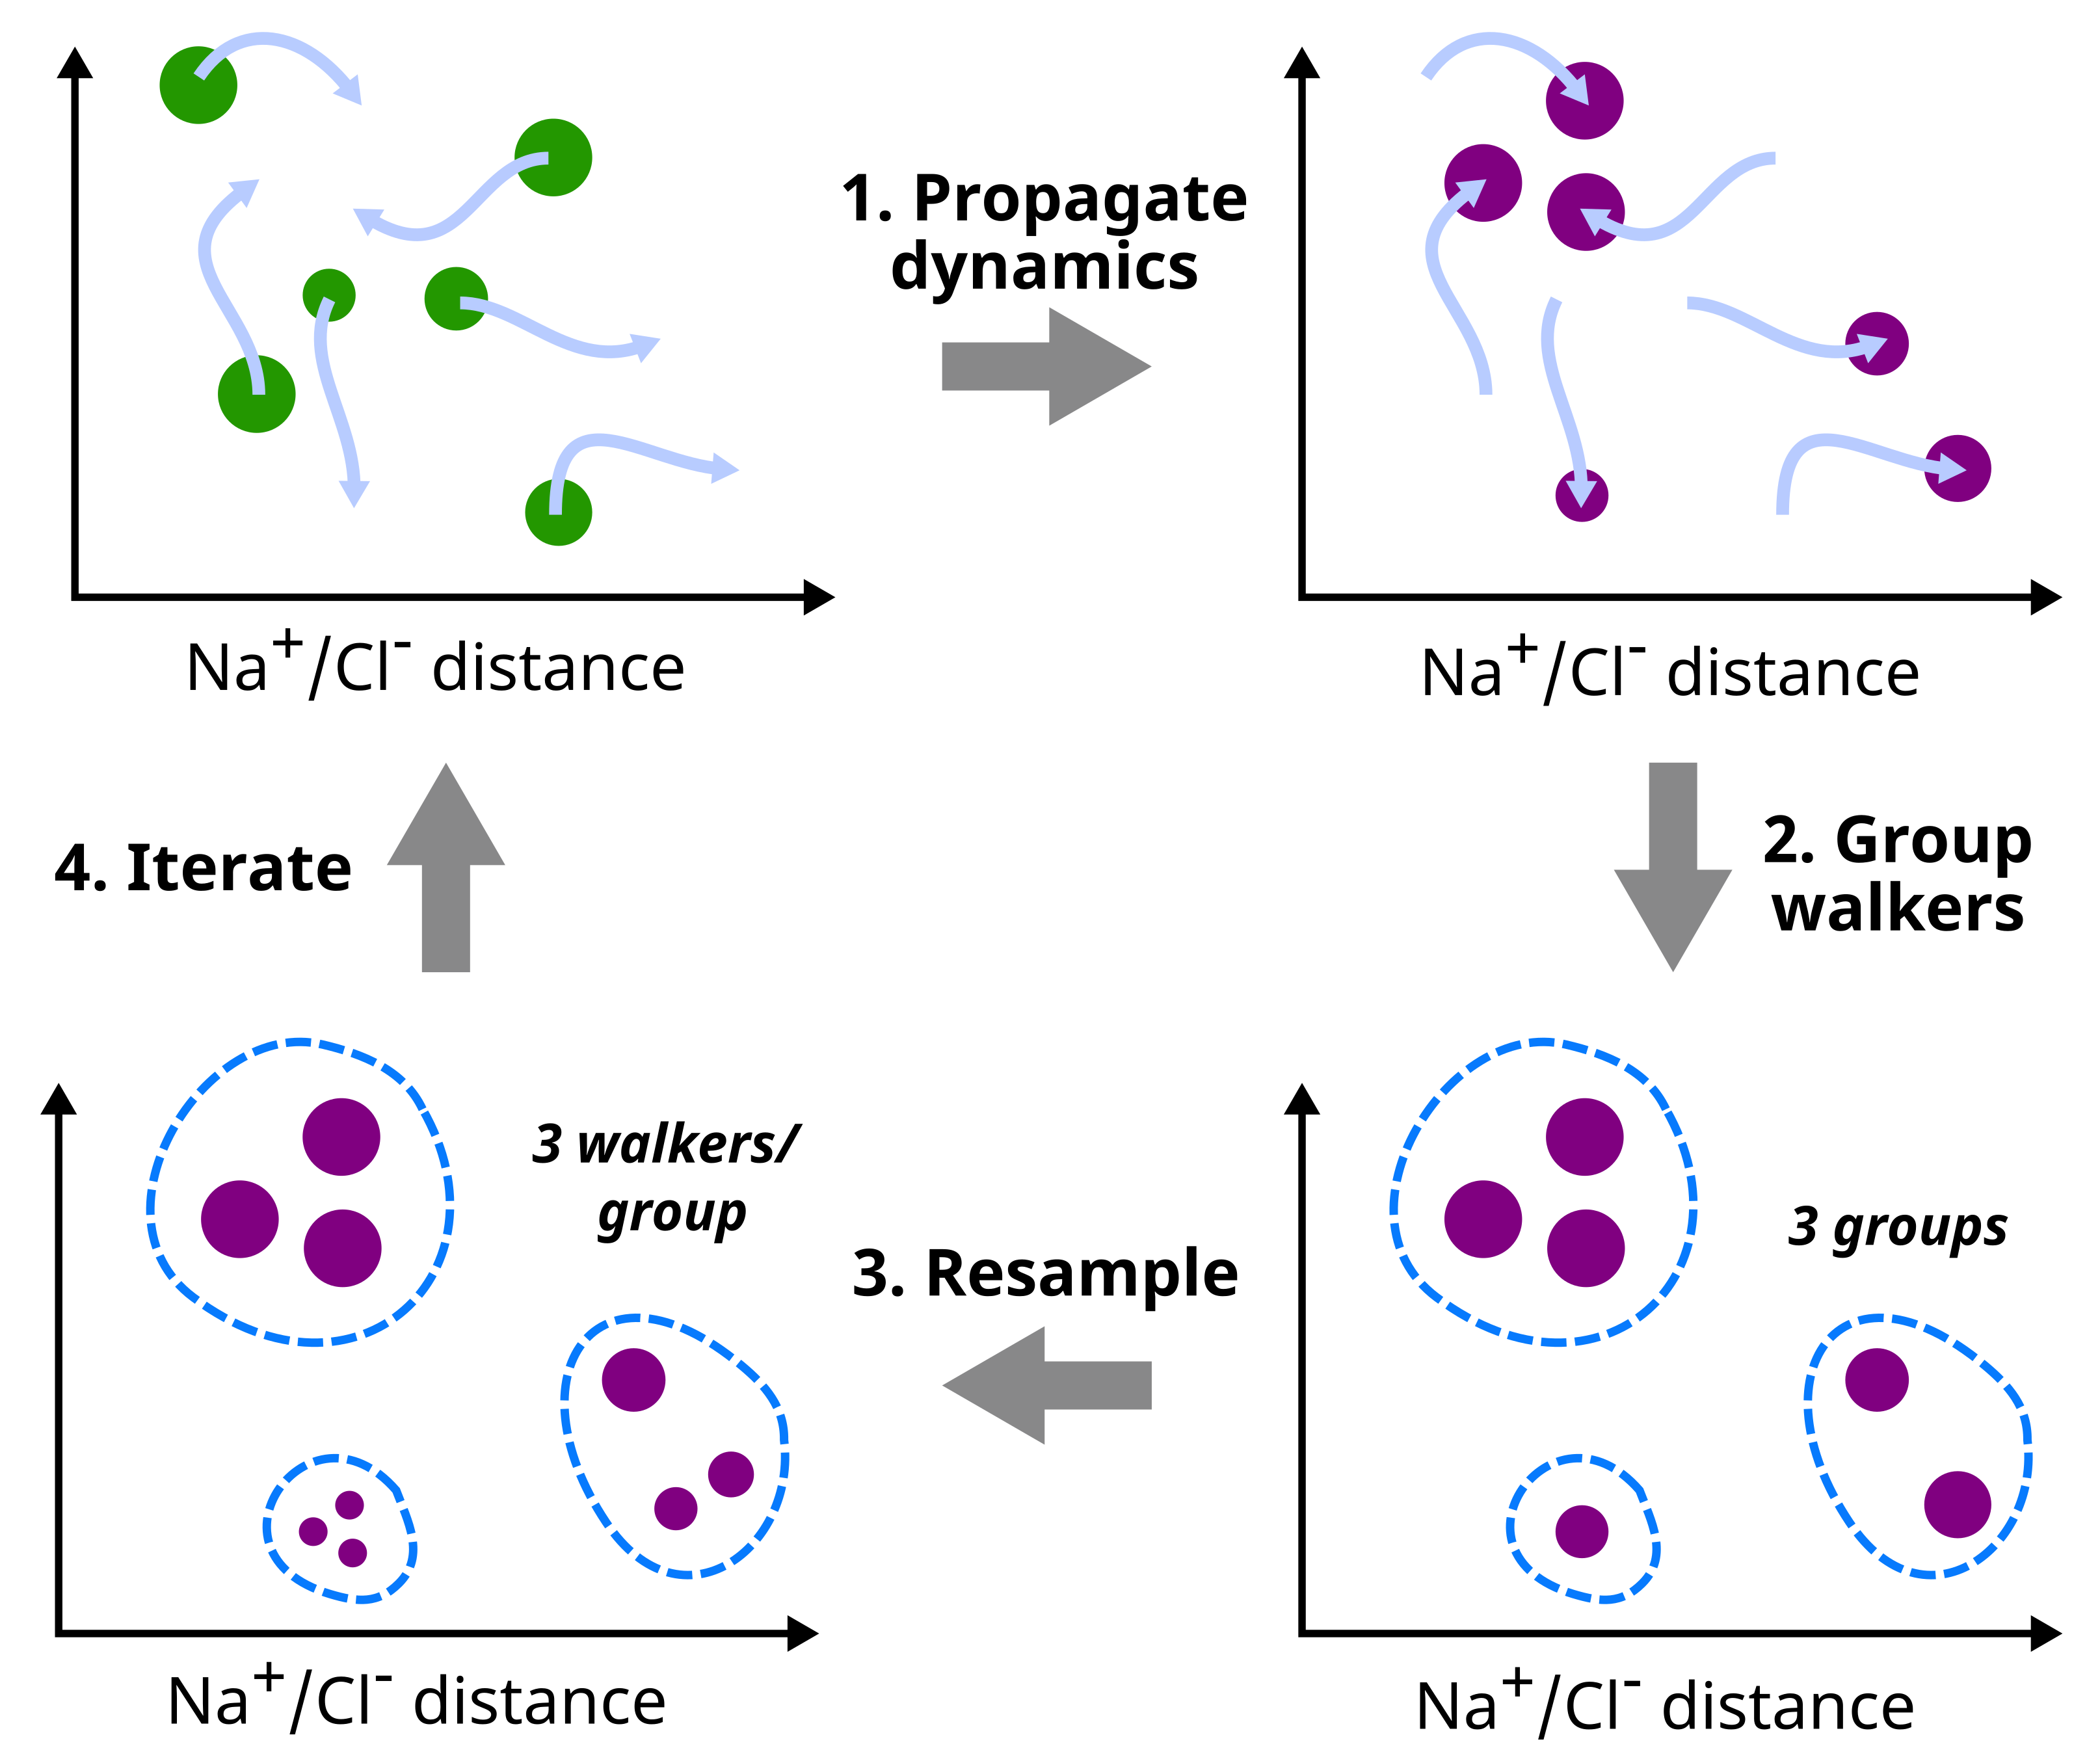
\includegraphics[width=\columnwidth]{figures/Figure3_binless.png}
\caption{Flow chart for simulating Na+/Cl- association using the new binless resampler module. 
After dynamics propagation in step 1, trajectories in each bin are grouped with the user-specified group.py function. 
In this example, trajectory walkers are grouped using k-means clustering.}
\end{figure}

\begin{verbatim}
  west:
    system:
      system_options:
        bins:
          type: RecursiveBinMapper
          base:
            type: RectilinearBinMapper
            boundaries:
              - [0, 2.60, 'inf']
            mappers:
            - type: BinlessMapper
              ngroups: [5] # Number of groups
              ndims: [1] # Number of grouping 
                         # dimensions
              group_function: group.kmeans
              at: [5]  # Location of binless mapper
                       # relative to base mapper
\end{verbatim} 

\textbf{Initiating a WE Simulation from Multiple Structures.} Ideally, a WE simulation is initiated from multiple pre-equilibrated structures that are representative of the initial state for the rare-event process of interest, e.g. using a conventional simulation or a separate WE simulation of the initial state.
Within the WESTPA framework, we refer to these structures as "basis states". 
If the simulation is run under non-equilibrium steady-state conditions, trajectories that reach the target state are “recycled” by terminating that trajectory and initiating a new trajectory with the same statistical weight from one of the basis states. 
Structural files (XML files in this tutorial) for basis states contain the coordinates and velocities, and are placed in separate, numbered folders within the \verb|bstates/| directory. 
Accompanying each XML file is a \verb|pcoord.init| text file which contains the progress coordinate value of that basis state. 
These progress coordinates are saved to the HDF5 file during the initialization process. 
The \verb|bstates/| directory also contains a reference file (\verb|bstates.txt|) that lists all of the available basis states. 
The \verb|bstates.txt| file is formatted with three columns, corresponding to the basis states’ names, associated probabilities, and folder name, respectively.
Additional basis states can be added as separate, additional lines at the end of the \verb|bstates.txt| file. 
The probability over all basis states must sum to one, and will be normalized by WESTPA during the initialization process to sum to one if the condition is not met.
Compared to the Basic WESTPA tutorial involving Na\textsuperscript{+}/Cl\textsuperscript{-} association \citep{bogetti_suite_2019}, the \verb|get_pcoord.sh| and \verb|runseg.sh| files are also modified such that \verb|$WEST_DATA_STRUCT_REF| now corresponds to the directory for each basis state and not the xml file itself.

\subsubsection{Running the WE Simulation}
As with previous versions of WESTPA, the simulation can be initialized using \verb|./init.sh| and run using \verb|./run.sh|. 
Alternatively, both steps could be executed consecutively using the new Python API by running the following command:

\begin{verbatim}
  $ python init_and_run.py
\end{verbatim}

The \verb|init_and_run.py| script will print out simulation updates to the console in real-time. 
An example \verb|runwe.slurm| file with commands for both methods of execution is provided for use with SLURM-like workload managers. 
We also provide a Jupyter notebook that demonstrates the steps for cleaning up, initializing, and running the WE simulation.

Note that this tutorial is using the new HDF5 trajectory storage framework, which will be explained further in \textbf{Advanced Tutorial 3.2}. 
To enable the use of the HDF5 framework in your own simulation, you may use the current tutorials directory as an example. 
The location of the trajectory h5 files will need to be specified in the \verb|west.cfg| file, and the appropriate restart and topology files will need to be copied to the locations specified in the \verb|get_pcoord.sh| and \verb|runseg.sh| files. 
You will also need to make sure that the file extensions for any trajectory files are readable by \verb|mdtraj.load()|, (e.g., Amber restart files must end in .ncrst) which simply requires renaming. 
To save disk space, trajectory files outputted by the dynamics engine can be deleted after every iteration in the \verb|post_iter.sh| file, which is located in the \verb|westpa_scripts/| directory.

\subsubsection{Monitoring and Analyzing the WE Simulation}

\textbf{Combining Multiple WE Simulations for Analysis.} To combine multiple WE simulations into a single aggregate simulation file for analysis, we can use the \verb|w_multi_west| tool, which creates a single \verb|multi.h5| file that contains the data from all of the \verb|west.h5| files of each WE simulation. 
Each WE iteration in the \verb|multi.h5| file contains all of the trajectory segments from the corresponding iterations of the individual WE simulations, all normalized to the total weight for that iteration. 
For backwards compatibility, a version of \verb|w_multi_west| for use with previously run WESTPA 1.0 simulations (v2020.XX) has been available since version 2020.04.

To apply the multitool to a combination of \verb|west.h5| files, place the \verb|west.h5| file for each simulation in a numbered directory starting with \verb|01/|. 
If all of the simulations used a custom grouping function (such as in \verb|group.py|), you must also include that file in the top-level analysis directory. 

The files will be organized as follows:
\begin{verbatim}
  01/
    west.h5
  02/
    west.h5
  group.py [if used in simulation]
\end{verbatim}

Next, in this directory, run the following to merge the \verb|west.h5| files:
\begin{verbatim}
  $ w_multi_west -m . -n 2
\end{verbatim}

The \verb|-m| flag specifies the path to your directories and the \verb|-n| flag specifies the number of WE simulations to combine for analysis. 
To combine auxiliary datasets, one can add either an \verb|--aux=NAME_OF_DATASET| flag for a specific dataset or an \verb|--auxall| flag for all auxiliary datasets; note that the inclusion of auxiliary datasets will substantially extend the time needed to combine the simulation data. 
The above \verb|w_multi_west --auxall| command will generate a list of WE simulation datasets to combine based on the datasets listed in \verb|01/west.h5| and generate a \verb|multi.h5| file with the combined simulation datasets. 
You may want to rename this file to \verb|west.h5| in order to apply the \verb|w_pdist| tool to the combined simulation dataset. 
Note that the \verb|w_multi_west| tool will only merge up to the \textit{N-1} WE iteration, ignoring the last WE iteration. 
The resulting \verb|multi.h5| file will not link to the individual iteration HDF5 files generated using the HDF5 framework.

\textbf{Post-Simulation Analysis.} As mentioned above, WESTPA 2.0 enables efficient post-simulation analysis of trajectory data by storing trajectory data in highly compressed HDF5 files. 
The \verb|w_crawl| tool can then be used to “crawl” through the trajectory data in single HDF5 files per WE iteration rather than millions of trajectory files.
Results from the analysis are written to a dataset in a new HDF5 file. 
Before crawling through an entire simulation dataset, we recommend that users first test their analysis scheme in the \verb|wcrawl_functions.py| file to ensure that the scheme works as expected. 
For this tutorial, we will only be using a single CPU core for these \verb|w_crawl| calculations but also include a sample script as an example of how to use \verb|w_crawl| on multiple CPU cores in parallel. 
The \verb|wcrawl_functions.py| file contains the main analysis code. 
This script first identifies the final frame of a segment’s parent trajectory file from the previous WE iteration and makes sure this is eventually combined with the trajectory segment from the current WE iteration. 
The inclusion of the parent structure at the beginning of the current iteration trajectory is necessary for using the crawled dataset with WESTPA’s kinetics analysis tools. 
In this example, trajectory coordinates of only Na\textsuperscript{+} and Cl\textsuperscript{-} are extracted using the MDTraj analysis suite and multiplied by 10 to convert from nm to \AA. 
Resulting per-iteration coordinate values are then saved to an array, which is subsequently saved to a \verb|coord.h5| file. 
The \verb|coord.h5| file is formatted similarly to a \verb|west.h5| file, where the new per-iteration values are stored under \verb|iterations/iter_{n_iter:08d}/coord|. 
To ease analysis, a \verb|copy_h5_dataset.py| script is provided to copy \verb|coord.h5|’s contents into a west.h5 file as an auxiliary dataset. 
Note that if you store a WESTPA simulation's trajectory HDF5 files in a separate directory from what is used in this tutorial, you need to specify the directory where the \verb|iter_XXXXXX.h5| files are located in the \verb|wcrawl_functions.py| file.

The \verb|run_w_crawl.sh| shell script runs the \verb|w_crawl| tool at the command line and provides options for running the tool in serial or parallel modes. 
In this tutorial example, we will run the \verb|w_crawl| tool in the serial mode using the \verb|--serial| flag, analyzing one WE iteration at a time on a single CPU core. 
While the serial mode is sufficient for “crawling” relatively small datasets, the parallel mode using the \verb|--parallel| flag is desirable for datasets with over 100 trajectory segments per WE iteration and/or hundreds of WE iterations. 
In the parallel mode, each CPU core of a single compute node analyzes a different WE iteration at the same time. 
To run the \verb|w_crawl| tool across multiple nodes, one can use the ZMQ work manager.
Once satisfied with the \verb|wcrawl_functions.py| and \verb|run_w_crawl.sh| files, run the \verb|w_crawl| tool locally:

\begin{verbatim}
  $ ./run_w_crawl.sh
\end{verbatim}

or on a multi-node cluster using the Slurm workload manager:

\begin{verbatim}
  $ sbatch run_w_crawl.sh
\end{verbatim}

To monitor the progress of the analysis, we examine the \verb|w_crawl.log| file, which contains analysis results for each WE iteration and each trajectory segment.
Finally, to copy the \verb|coord.h5| file to the \verb|west.h5| file, run the \verb|copy_h5_dataset.py| script.

\subsubsection{Conclusion} After completing this tutorial, users will gain an understanding of how to configure the upgraded resampler module for using a binless scheme, initiate a WE simulation from multiple structures using the new HDF5 trajectory storage framework, and apply the \verb|w_multi_west| and \verb|w_crawl| post-simulation analysis tools. 

\subsection{Advanced Tutorial: Simulations of Membrane Permeation by 1-Butanol}
\label{tut:mem-perm-adv}

\subsubsection{Introduction}
The ability of a drug-like molecule to cross (or permeate) a lipid bilayer has been of great interest to drug discovery \citep{zhang_mechanistic_2022}, but is challenging to simulate due to the long timescales involved. 
In this tutorial, we will use WESTPA 2.0 to simulate pathways for membrane permeation by a small molecule (1-butanol) and calculate the permeability coefficient. 
Our WE protocol employs and explains two new features in WESTPA 2.0 \citep{russo_westpa_2022}: (i) the Minimal Adaptive Binning (MAB) scheme \citep{torrillo_minimal_2021}, and (ii) the HDF5 framework for efficient restarting, storage, and analysis of a WE simulation.

\textbf{Learning Objectives.} This tutorial demonstrates how steady state WE simulations can be used to generate pathways and permeability coefficients for membrane permeation by a small molecule.  
Specific learning objectives include:
\begin{enumerate}
    \item How to set up a double membrane bilayer system for permeability studies;
    \item How to use the highly scalable HDF5 framework for more efficient restarting, storage, and analysis of simulations;
    \item How to apply the minimal adaptive binning (MAB) scheme.
\end{enumerate}

\subsubsection{Prerequisites}
In addition to completing the Basic and Intermediate WESTPA Tutorials \citep{bogetti_suite_2019}, a prerequisite to this advanced tutorial is completion of the above \textbf{Advanced Tutorial \ref{tut:mem-perm-adv}}. 
Also required is a working knowledge of the CHARMM-GUI membrane builder, PACKMOL, OpenEye Scientific’s OEChem and Omega toolkits (for system preparation only), MDTraj analysis suite, and the OpenMM 7.6 dynamics engine (for running WE). 

\textbf{Computational Requirements.} The membrane permeability tutorial simulation runs best using, at minimum, a dual-GPU workstation. 
For this tutorial, simulations were tested with a compute node containing both a NVIDIA Titan X (Pascal) GPU and a NVIDIA GTX 1080 GPU, as well as a 16-core Intel Xeon X5550 CPU running at 2.67 GHz with a total of 100 GB of system memory. 
In the case a user does not have a GPU and only CPUs, switch between OpenMM's GPU and CPU platforms by changing the platform name in line 22 of \verb|memb_prod.py| to \verb|CPU| instead of \verb|CUDA|. 
The complete tutorial simulation run length (37 iterations) required \textasciitilde4 days of continuous wall clock time on both GPUs, as well as \textasciitilde30 GB of hard disk space with the HDF5 framework and MAB options turned on.

This tutorial uses the OpenMM 7.6 dynamics engine \citep{eastman_openmm_2017} and MDTraj 1.9.5 analysis suite ({\url{https://www.mdtraj.org/1.9.5/index.html}}) for progress coordinate calculations. 
Force fields used in this tutorial can be installed via openmmforcefields ({\url{https://github.com/openmm/openmmforcefields}}). 
System setup and equilibration were performed separately using OpenMM. 
In order to run the companion Jupyter notebook, nglview, matplotlib are required for visualization purposes. 
Other dependencies, including NumPy and MDTraj, are installed with WESTPA 2.0 itself.

\textbf{Quick Start for this Tutorial.} Users can run the following command within the \verb|tutorial-7.6/| directory to install all the software dependencies to an existing conda environment:

\begin{verbatim}
  $ conda env update --name <your WESTPA conda env> 
                               --file environment.yml
\end{verbatim}
\pagebreak

\subsubsection{Preparing the simulation}
The following preparation steps have already been completed and are presented to instruct the reader on how to prepare similar systems for WE simulation.

Our system consists of a 1-palmitoyl-2-oleoyl-sn-glycero-3-phosphatidylcholine (POPC) membrane bilayer. 
The 1-butanol-double POPC membrane bilayer system was prepared by piecing together several smaller molecular systems in the following way.
First, a single POPC membrane bilayer was generated using CHARMM-GUI’s membrane builder with 50 lipids per leaflet and zero salt concentration. 
This membrane was then equilibrated using a single GPU with the OpenMM dynamics engine using the standard CHARMM-GUI procedure. 
The membrane plus the outer aqueous layer to the membrane, once combined, (see \textbf{Figure \ref{fig:bilayer-butanol}}) was equilibrated for an additional 500 ns.
A 2D representation of 1-butanol was generated from an input SMILES string (CCCCO) using OEChem, and converted to a 3D structure using the Omega TK toolkit. 
The 3D structure of 1-butanol was then solvated with a 2 nm slab of water molecules at a density of 1 gm/cm\textsuperscript{3} using PACKMOL along with the OEChem TK and Omega TK toolkits from OpenEye.
Finally, the full double-membrane bilayer system was assembled by placing the butanol-embedded slab of water at the origin, with a single-membrane system at each z-edge of the water slab. 
The resulting system was then subjected to energy minimization and equilibrated before the initiated WE simulations of butanol permeating the membrane bilayer were initialized. 

\begin{figure}[t]
\centering
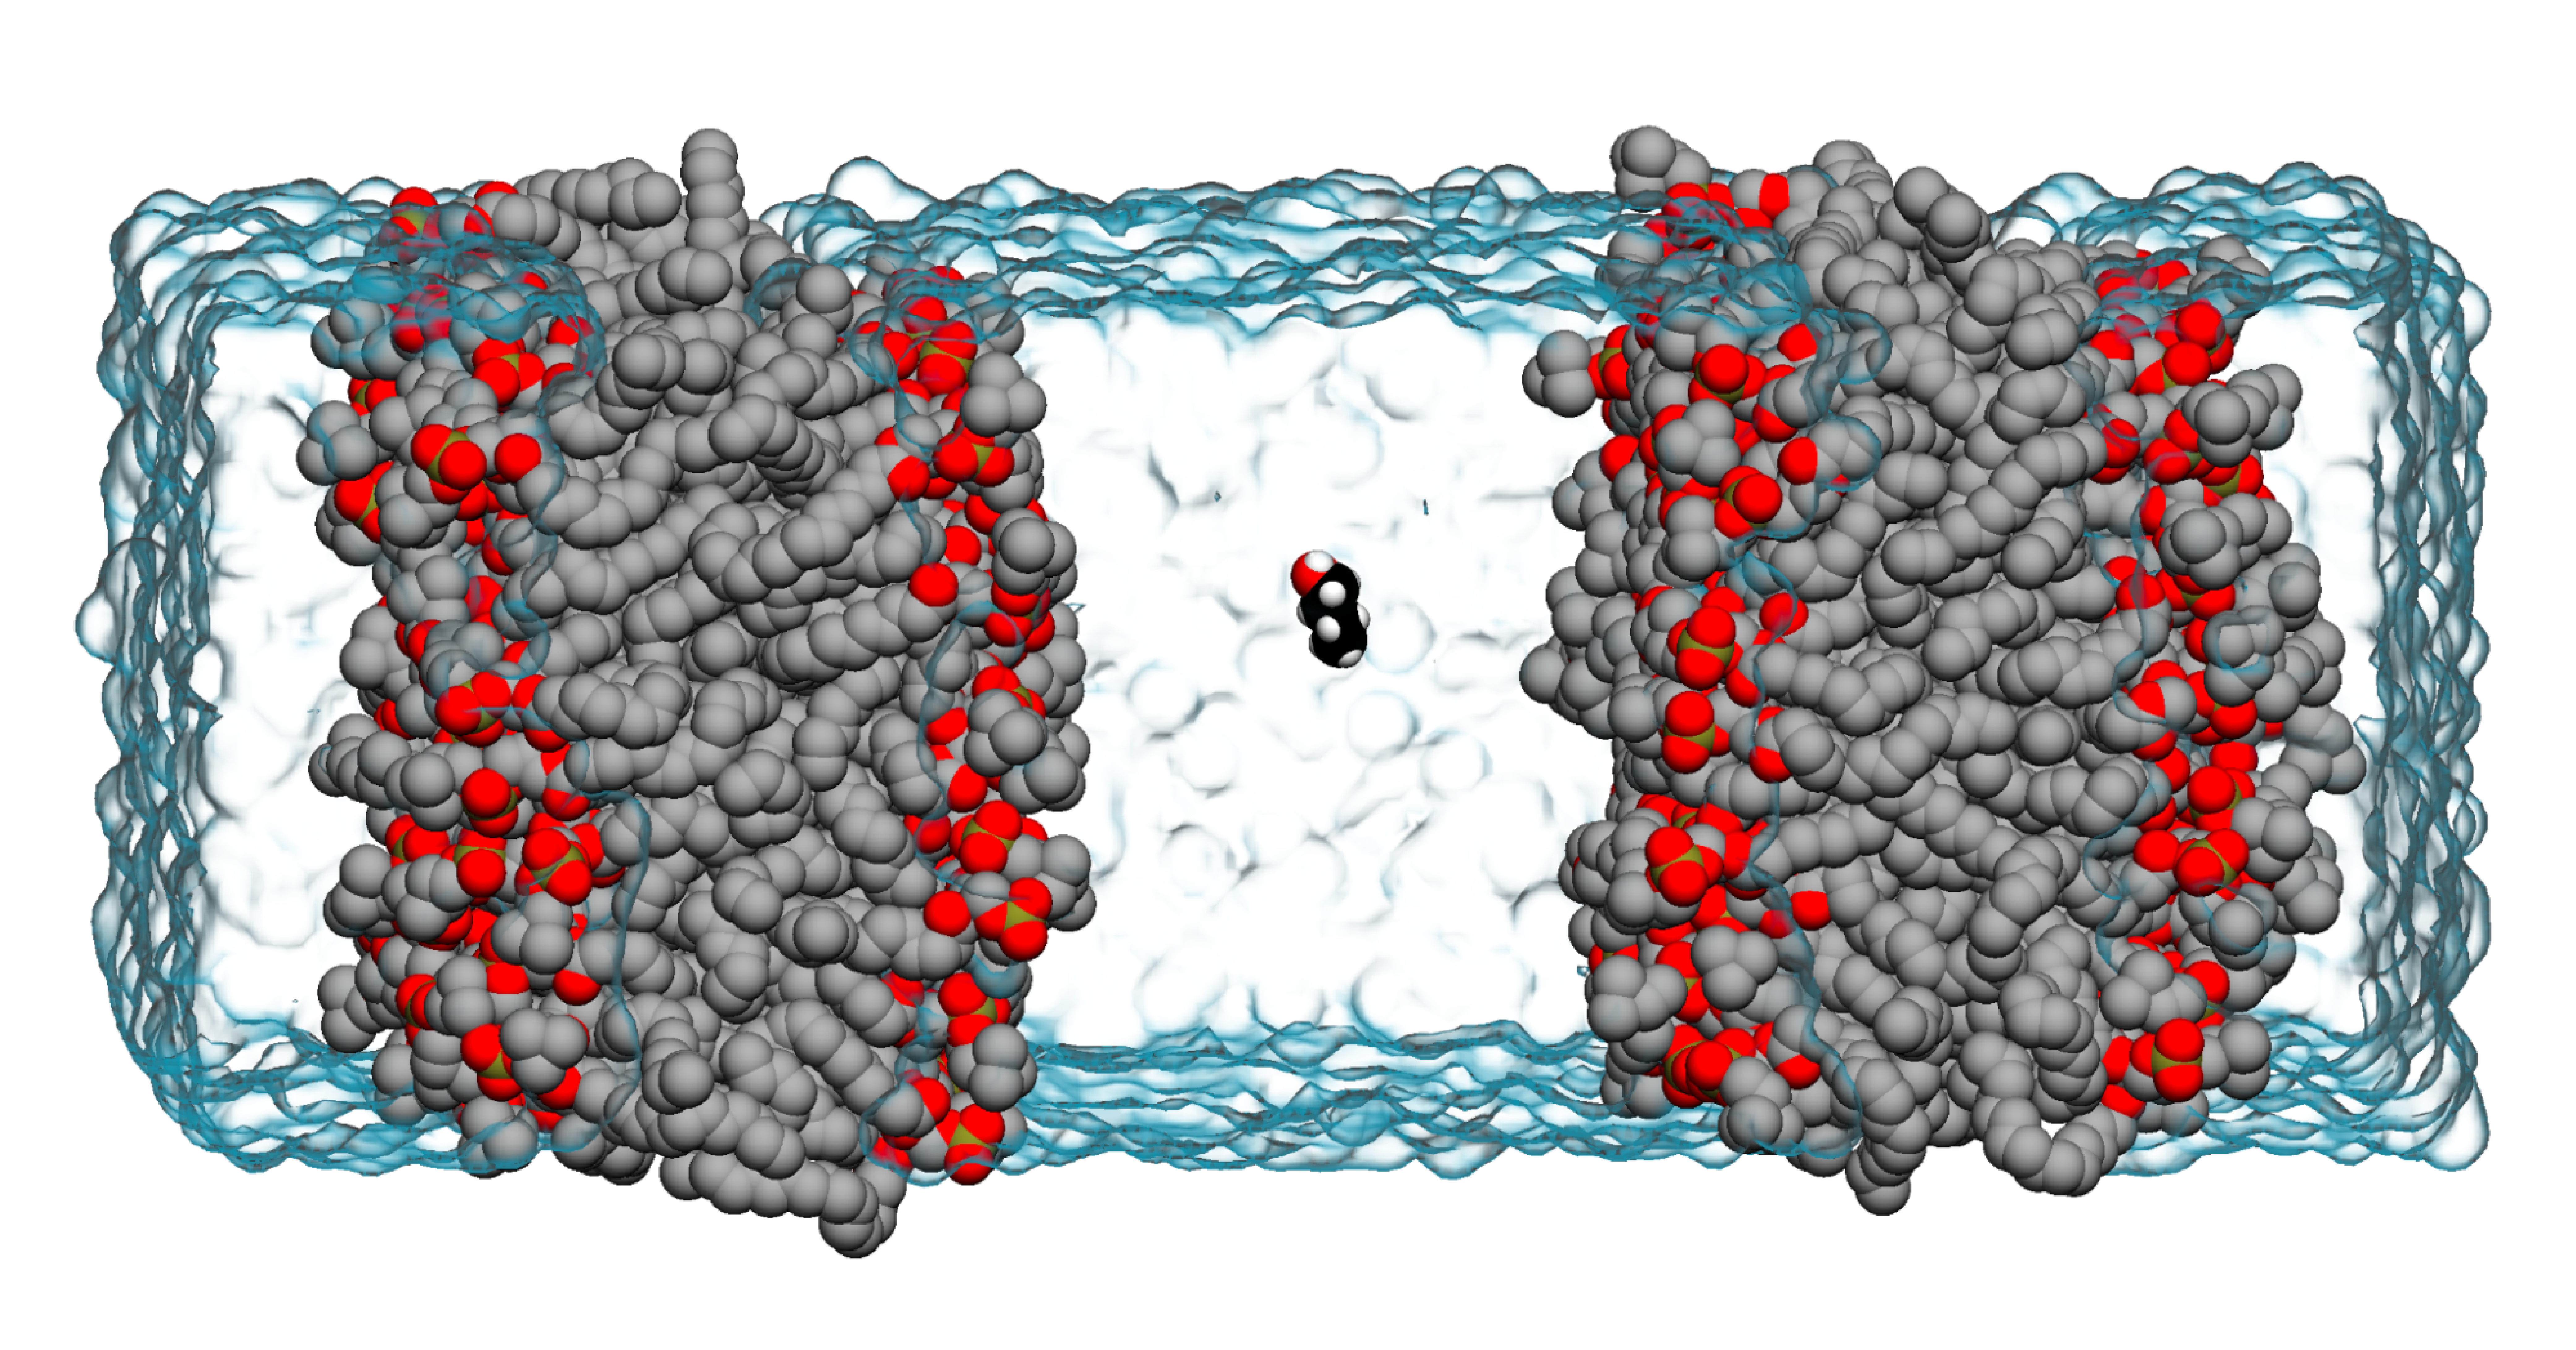
\includegraphics[width=\columnwidth]{figures/Figure4_membrane.pdf}
\caption{The equilibrated double-membrane bilayer system used for initiating WE simulations of membrane permeation by 1-butanol in this tutorial. 
Both the POPC membrane bilayers (gray; hydrogens removed for clarity) and 1-butanol (black) are represented in van der Waals representation, while layers of explicit water molecules are shown as a transparent blue surface.}
\label{fig:bilayer-butanol}
\end{figure}

\textbf{The System.} In this tutorial, we will run a WE simulation of 1-butanol crossing one membrane of a double POPC membrane bilayer system. 
To run the WESTPA 2.0 simulation, the AMBER LIPID17 force field is applied to all POPC lipids, explicit water molecules are represented by the TIP3P model, while the parameters for 1-butanol were taken from the GAFF 2.11 force field. 
All force field parameters were applied using the openmmforcefields Python package.

\textbf{Progress Coordinate.} The progress coordinate (z) is defined as the (signed) distance from the center of mass (COM) of the butanol molecule to that of the closest membrane. 
The width of a single leaflet of the membrane is roughly 2 nm, so a z < -2 nm, between -2 nm and 2 nm, or >2 nm indicates that the butanol molecule has not yet crossed, is currently crossing, or has crossed the membrane, respectively. 
A target state of z $\geq$3.5 nm is used to recycle trajectory walkers. 
The actual computation is performed by measuring the signed distances between the COMs of butanol and each of the two membranes, z\textsubscript{1} and z\textsubscript{2}, using the MDTraj analysis suite and then taking the larger value of the two, z=max(z\textsubscript{1}, z\textsubscript{2}).

\textbf{Preparing the Simulation Environment.}  Once we have constructed and equilibrated the 1-butanol membrane system, we will prepare the WESTPA system environment. 
First, we will analyze the equilibrated double membrane bilayer system to define an initial progress coordinate. 
The progress coordinate, equilibrated coordinate file (e.g. XML file), and \verb|bstates.txt| file describing the initial basis states are placed in the \verb|bstates/| directory. 
Second, we will edit the \verb|west.cfg| file with options for using the MAB scheme and HDF5 framework. 
To initialize the WESTPA 2.0 environment, we will run \verb|./init.sh|. 
This command will source the WESTPA 2.0 environment, construct the \verb|seg_logs/|, \verb|traj_segs/|, and \verb|istates/| directories, and will run the \verb|w_init| command with the correct settings for the target state (z = 3.5 nm) and the basis states constructed above.

\textbf{Adaptive Binning using the MAB Scheme.} By default, this tutorial uses a manual, fixed binning scheme, but can be modified to use the Minimal Adaptive Binning (MAB) module, which adaptively positions bins along the progress coordinate. 
To enable this adaptive binning scheme, uncomment the MAB-related lines in the \verb|west.cfg| file, which specify the \verb|MABBinMapper| as the primary bin mapper type, and comment the lines related to the inner \verb|RectilinearBinMapper|. 
Next, define \verb|n_bins| (the number of MAB bins placed per progress coordinate dimension) in the same section of the \verb|west.cfg| (e.g., if a two-dimensional progress coordinate is being used, \verb|[20, 20]| indicates 20 bins in each dimension). 
It is important to note that if the recycling of trajectories at a target state is desired within the MAB framework, recursive bins must be specified by adding a \verb|MABBinMapper| inside of a \verb|RecursiveBinMapper| outer bin and defining the target state in terms of the recursive outer bins. 
An example of a MAB recursive binning scheme is shown below:

\newpage
\begin{verbatim}
  west:
    system:
      system_options:
        bins:
          type: RecursiveBinMapper
          base:
            type: RectilinearBinMapper
            boundaries:
              - [-inf, -44, 34, inf]
            mappers:
            - type: MABBinMapper
              nbins: [20] # Number of bins
              direction: [0] # Split both directions
              skip: [0] # Bin along this dimension
              at: [0]  # Location of MAB mapper
                             relative to base mapper
\end{verbatim}

In the above example, the \verb|at| option in the last line specifies which outer bin to place the MAB scheme inside of range \verb|[-44, 34]|. 
For a two-dimensional progress coordinate, this option will require a list with two values, one for each dimension. 
The \verb|nbins| option specifies the number of MAB linear bins that will be used inside the bin, plus two more bins for extrema and bottleneck trajectories, respectively. 
Optional \verb|direction|, \verb|skip| and \verb|mab_log| parameters can also be specified for the MAB scheme. 
The \verb|direction| parameter (0, -1, or 1) can be used to specify the direction along the progress coordinate for splitting of trajectories, where 0 indicates both directions, -1 indicates the direction of decreasing values along the progress coordinate, and 1 indicates the direction of increasing values along the progress coordinate. 
The \verb|skip| parameter  (1 or 0) designates whether a particular dimension along the progress coordinate will be binned during the simulation, but will be used to define the target state (1 indicates that the dimension will be skipped for binning and 0 indicates that the dimension will not be skipped for binning). 
The \verb|mab_log| parameter, when enabled with \verb|true|, will print MAB-related statistics such as the progress coordinate values of extrema walkers to the \verb|west.log| file. 
Multiple MAB schemes can be added to a recursive binning setup, but only one MAB scheme may be used per each outer bin.

If users choose to combine the application of the MAB scheme with the weighted ensemble steady-state (WESS) plugin \citep{bhatt_steady-state_2010}, which reweights trajectories towards a non-equilibrium steady state, they must provide fixed bins for the reweighting procedure. 
The positions of these fixed bins can be specified in the WESS plugin section of the \verb|west.cfg| file:
\newpage
\begin{verbatim}
  plugins:
    - plugin: westpa.westext.wess.WESSDriver
      enabled: true
      do_reweighting: true
      window_size: 0.75
      bins:
        type: RectilinearBinMapper
        boundaries:
          - ['-inf', 0.5, 1.0, 1.5, 2.0, 2.5, 'inf']
          
\end{verbatim}

\begin{figure}[t]
\centering
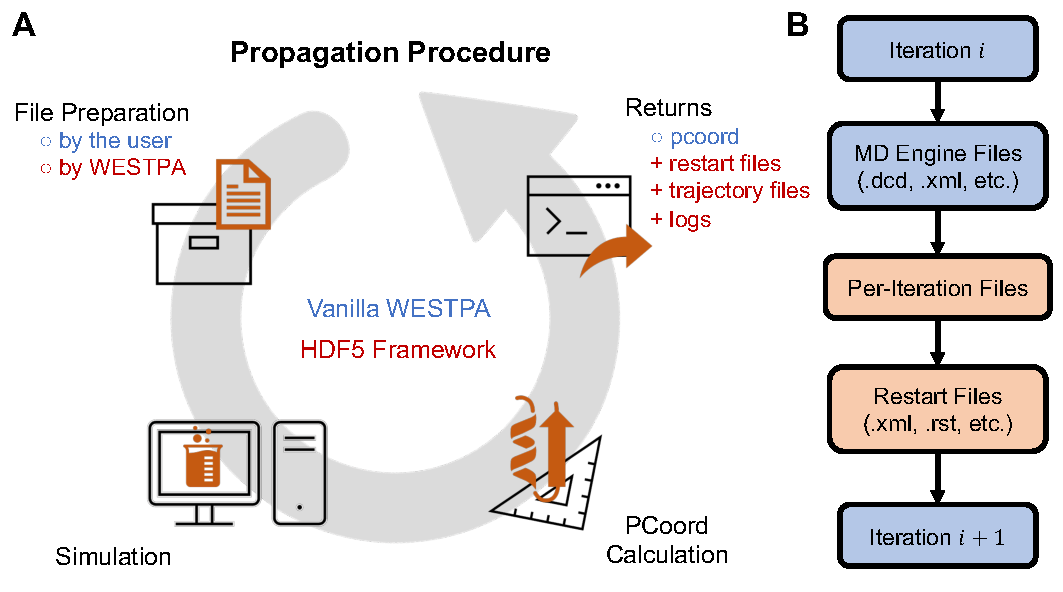
\includegraphics[width=\columnwidth]{figures/Figure5_membrane.pdf}
\caption{Diagrams showing the differences in the propagation procedure between a vanilla WESTPA run and a run with the HDF5 framework. 
A) Procedures for propagating one WE iteration using the original WESTPA 1.0 framework (blue text) and WESTPA 2.0 HDF5 framework (red text). 
Using the WESTPA 2.0 HDF5 framework, the WESTPA software prepares the input files while the user is responsible for returning the progress coordinate (pcoord), restart, trajectory, and optional log files. 
B) Workflow for using the WESTPA 2.0 HDF5 framework. 
Blue: Steps and files from the original WESTPA 1.0 procedure. 
Red: Files generated or prepared by the WESTPA 2.0 HDF5 framework. }
\label{fig:we-hdf5}
\end{figure}

\textbf{HDF5 Framework.} The setup for a WESTPA simulation with the HDF5 framework is similar to a vanilla one with the addition of the following procedures, which are a more detailed list of the same steps discussed briefly in \textbf{Advanced Tutorial \ref{tut:binless}} above:
\begin{enumerate}
    \item An \verb|iteration| entry was provided in \verb|west.cfg| under \verb|west.data.data_refs| to specify where and how the per-iteration HDF5 files should be saved and named. 
    \item All the necessary files needed for propagating the next segment, such as state/restart and topology files, are passed on to WESTPA through the environment variable, \verb|$WEST_RESTART_RETURN|, after initialization and propagation of each iteration (\textbf{Figure \ref{fig:we-hdf5}A}). 
    This information is typically placed in the \verb|get_pcoord.sh| and \verb|runseg.sh| files. 
    \item All the trajectory files, and topology files if the topology is not stored as part of the trajectory file, are provided to WESTPA through the environment variable, \verb|$WEST_TRAJECTORY_RETURN|, after the propagation of each iteration. 
    This, again, is typically placed in the \verb|get_pcoord.sh| and \verb|runseg.sh| files. 
    The coordinates of the basis states can be provided through the environment variable during initialization to be stored as the “trajectories” of the zero-th iteration. 
    Note that the procedures described in step 2 and 3 are similar to how the progress coordinates are returned through \verb|$WEST_PCOORD_RETURN| in the vanilla WESTPA simulation. 
    The trajectory and restart files will be saved as part of the per-iteration HDF5 files. 
    In turn, these files do not need to be located and copied over to the directory for propagating the next segment, and they will be automatically extracted and put into the segment folder by WESTPA instead (Figure \textbf{\ref{fig:we-hdf5}B}).
\end{enumerate}

These additional procedures simplify the data management on the user’s end for two reasons. 
First, all the trajectories are stored in a standard way which enables fast and easy access to these trajectories with their associated WE-related data using the newly added analysis module (see Section \ref{tut:binless-running}). 
Second, the restart/state files are much easier to locate as when they are generated than when they are needed in the next iteration, so letting the users pass trajectory and restart files to WESTPA for it to manage frees users from tracking those files themselves which would require the critical knowledge of how two WESTPA-assigned environment variables work (namely, \verb|$WEST_CURRENT_SEG_INITPOINT_TYPE| and \verb|$WEST_PARENT_DATA_REF|). 

For this membrane permeation example, the per-iteration HDF5 files are saved in a folder named \verb|traj_segs/| and named following the pattern \verb|iter_XXXXXX.h5|. 
The basis states are returned to WESTPA in \verb|get_pcoord.sh| as both the “trajectories” of the zero-th iteration and the restart files for propagating the first iteration and recycled walkers. 
The dynamics is propagated using OpenMM for 100 ps for each iteration, and the output trajectory files and state XML files are returned to WESTPA in \verb|runseg.sh|. 
These files are deleted once they are returned in order to save disk space. 
See the sample project setup files for detail.

\subsubsection{Running the WE Simulation}
Similar to other examples, the simulation can be run using \verb|./run.sh| from the top-level permeability tutorial directory.

\subsubsection{Analyzing the WE Simulation}
The analysis of the membrane permeation simulation can be found in the accompanying Jupyter notebook titled Membrane Permeability Tutorial (Analysis). 
In this tutorial notebook, we demonstrate how to extract a complete, continuous pathway of a membrane-crossing event and calculate the incoming flux to the target state from the WE membrane permeation simulation. 
Note that this tutorial assumes that you already have a completed simulation using the HDF5 framework with at least one crossing event (\textasciitilde40 iterations).

\subsubsection{Conclusion}
In this tutorial, we have illustrated the relative ease in which one may use the WESTPA 2.0 software package to perform advanced WE path sampling simulations of membrane permeation for a small molecule (butanol). 
Using a single workstation with two GPUs, our WE simulation can generate membrane permeation events within a few days of wall-clock time. 
WE simulations, when using the WESTPA 2.0 HDF5 framework and MAB binning scheme, are relatively cost effective, both in terms of total computing time and disk storage.

\subsection{Advanced Tutorial: Analysis and restarting with haMSMs: NTL9 Protein Folding}
\label{tut:hamsm-adv}

\begin{figure}[t]
\centering
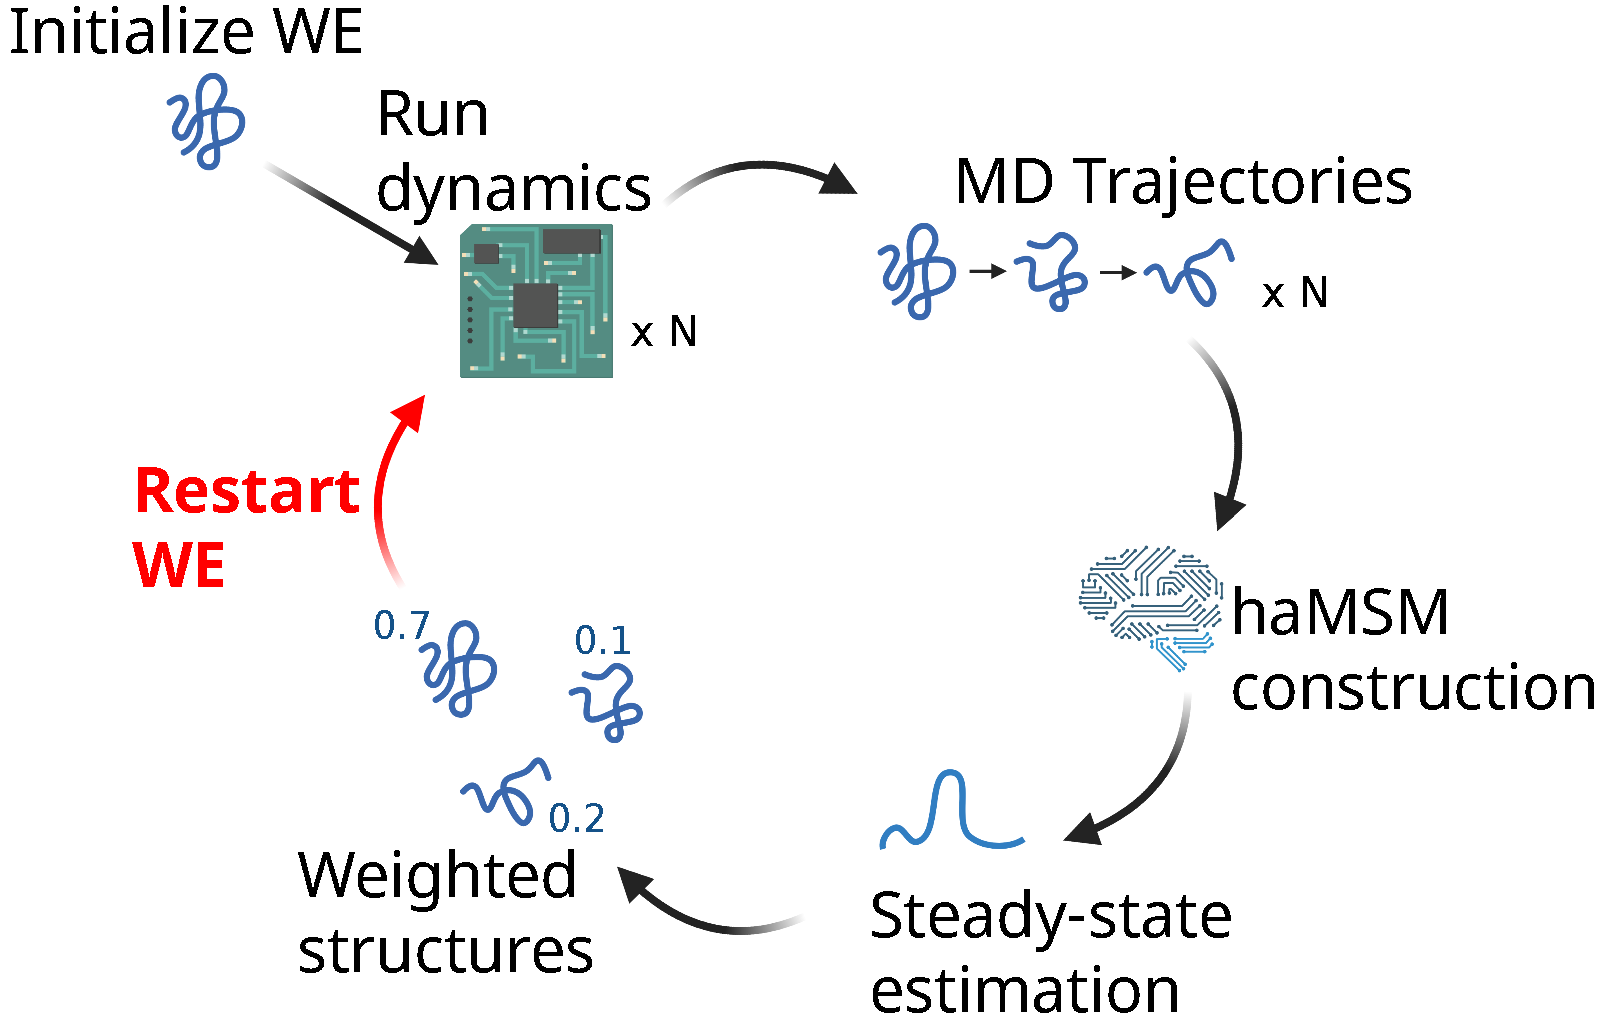
\includegraphics[width=\columnwidth]{figures/Figure6_haMSM.pdf}
\caption{Schematic of haMSM restarting procedure. 
Trajectories from one or more WE runs are used together to build an haMSM. 
An estimate of steady-state is obtained from the haMSM, and is used to assign weights to all sampled structures. 
New WE runs are initiated from these steady-state weighted structures, and the procedure repeats. 
Figure reprinted with permission from \citep{russo_westpa_2022}. 
Further permission related to the source material should be requested from ACS.}
\label{fig:hamsm}
\vspace{-0.25cm}
\end{figure}

\subsubsection{Introduction}
Although the WE strategy provides an efficient framework for unbiased rare-event sampling, slow relaxation to steady state and impractically large variance in rate constant estimates may still be limiting factors for complex systems.
History-augmented Markov state models (haMSMs) have been demonstrated to provide estimates of steady state from transient, relaxation-phase WE data, which can be used to start new WE simulations \citep{copperman_accelerated_2020}. 
As shown in \textbf{Figure \ref{fig:hamsm}}, the haMSM plugin for the WESTPA 2.0 software package automatically constructs an haMSM from one or more independent WE simulations to estimate steady-state observables and then can automatically initiate new simulations from those estimates and iteratively repeat this procedure when those simulations complete. 
The underlying haMSM analysis library, \verb|msm_we|, can also be used to perform stand-alone haMSM analysis of existing WESTPA data.



\textbf{Learning Objectives.}  This tutorial demonstrates the use of an haMSM restarting workflow in WE simulations of the ms-timescale folding process of the NTL9 protein. 
Specific objectives are:
\begin{enumerate}
    \item How to apply the haMSM plugin for periodic restarting of simulations;
    \item How to use the \verb|msm_we| package to build an haMSM from WE data;
    \item How to estimate the distribution of first passage times from the haMSM, using \verb|msm_we|.
\end{enumerate}

\subsubsection{Prerequisites} The Basic and Intermediate WESTPA Tutorials \citep{bogetti_suite_2019} should be completed before running this tutorial.

\textbf{Computational Requirements.} This tutorial can be completed on a computer with a single NVIDIA GTX 1080 GPU and a 2.4GHz Intel Xeon E5-2620 in 90 min. 
The WE simulation will generate \textasciitilde5 GB of data, though on a typical cluster filesystem, overhead associated with data redundancy may increase this to \textasciitilde15 GB. 
A version of the Amber software package compatible with Amber 16 restart and topology files must be installed to propagate the dynamics and calculate the WE progress coordinate. 

The \verb|msm_we| Python package must also be installed, which can be done by first cloning the repository and then installing it into your existing conda environment (with WESTPA already installed) by running:
\begin{verbatim}
  $ git clone https://github.com/westpa/msm_we
  $ cd msm_we 
  $ conda env update --name <your WESTPA conda env> 
          --file environment.yml
\end{verbatim}

\subsubsection{Plugin functionality}
Once we initiate a WESTPA run with the haMSM plugin enabled, the plugin will execute a series of independent WE simulations (runs) from the same starting configuration for the number of WE iterations specified in \verb|west.cfg|. 
For this tutorial, the runs will not use the HDF5 trajectory-saving framework.

If none of the WE runs have reached the target state, the haMSM plugin will sequentially extend each run for a number of iterations specified in \verb|west.cfg|. 
This extension procedure will be repeated until at least one run has reached the target state. 
For consistency, all of the other runs in the set will be extended to match the length of this run. 
As a result of this extension procedure, runs used for the first restart may be longer than runs in subsequent restarts.

After completing the extension procedure, the plugin will construct an haMSM from these runs, and estimate the steady-state distribution and flux into the target state. 
All structures sampled by the set of runs are used to build this haMSM, and are then weighted according to a steady state. 
Note that this haMSM uses only the first and last frame of each WE iteration, which effectively sets the lag-time equal~ to~ the~ WE~ resampling~ time. A~ number of~ plots~ are~ automatically generated from the model. 
The flux profile, shown in \textbf{Figure \ref{fig:flux-profile}}, provides an important metric of convergence, and should be examined carefully. 
A flatter flux profile indicates more converged weighted ensemble.

\begin{figure}[t]
    \centering
    \vspace{-0.25cm}
    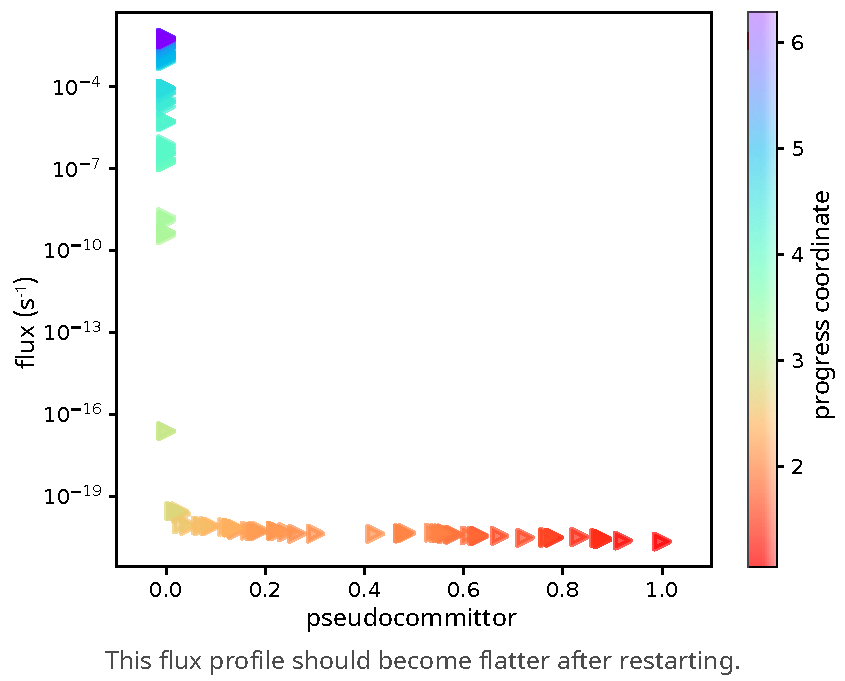
\includegraphics[width=\columnwidth]{figures/Figure7_committor.pdf}
    \caption{Sample flux profile generated by haMSM restarting plugin after a restart. 
    The x-axis is labeled "pseudocommittor", since these are committor values generated from a unidirectional path ensemble. 
    This plot should flatten in successive restarts until steady state is reached.
    The color scale indicates the progress coordinate associated with each pseudocommittor---notably, most of the dynamic range in committor-space is restricted to a small range of progress coordinate values. 
    This image can be found in restart0/plots/psuedocomm-flux\_plot\_pcoordcolor.pdf after restart is performed.}
    \vspace{-0.25cm}
    \label{fig:flux-profile}
\end{figure}

A new set of runs from the resulting weighted structured are initialized. 
These runs are correlated but independent from this point onward.
As a technical note, when initializing the new WE simulations, these structures are used as "start states". 
Within the WESTPA 2.0 framework, start states are a third category of state, in addition to basis states and target states. 
Like basis states, start states are used for seeding trajectory walkers when initializing a simulation with \verb|w_init|; however, \textit{unlike} basis states, start states are not used after this point and walkers reaching the target state will \textbf{not} be recycled into start states but rather only to the basis states. 
The new WE runs are executed for the number of WE iterations specified in \verb|west.cfg|, in series. 
At this point, the model is saved, a new restart is prepared, and the process repeats from that point onward.

Please see \citep{russo_westpa_2022, copperman_accelerated_2020} for more theoretical background on the models used by this plugin.
\subsubsection{Preparing the system}

\noindent\textbf{The system.} For our simulation of the NTL9 protein folding process, we use a stochastic Langevin thermostat with low-friction (collision frequency $\gamma$ = 5 ps\textsuperscript{-1}) and a generalized Born implicit solvent model. 
The system consists of \textasciitilde600 atoms. 
We will use the haMSM restart plugin to automatically perform three independent WESTPA runs serially before constructing an haMSM. 
A single restart will be performed from the haMSM steady state estimate, and then WE simulation will be continued for another 106 WE iterations for each of the three runs.

To reduce runtime for this tutorial, we provide a partially completed set of three independent WE simulations. 
In this set of simulations, the first two runs have completed, and the third is nearing completion. 
None of these simulations have yet reached the target state. 

After continuing this set of WE simulations, the third simulation will finish and reach its maximum number of WE iterations. 
With very high probability, none will have reached the target folded state, and pre-restart extensions will be triggered. 
The initialized runs were chosen such that it is unlikely that the third run will reach the target state before the next restart. 
However, it is possible that in the remaining few WE iterations of the third simulation, this simulation will reach the target state, in which case we will skip the extension procedure.

After a single round of extensions, the target state should be reached in run 2, though not necessarily runs 1 or 3. 
We will construct the haMSM from the three extended runs, and restart a new set of three runs from the steady-state estimates.

\textbf{Structure of Plugin-Specific Files.} A list of important files used and generated in \verb|$WEST_SIM_ROOT| by the haMSM plugin is shown in \textbf{Table \ref{tut:hamsm-table}}.

\begin{table}[t]
\caption{haMSM plugin organization and file explanations}
\label{tut:hamsm-table}
\centering
\begin{tabular}{| l | l |}
\hline
\verb|restart.dat| & Tracks current restart/run \\
\hline
\verb|restart_| & User provided on start, \\
\verb|initialization.json| & modified by plugin during run \\
\hline
\verb|west.h5| & Generated by WESTPA \\
{} & for the currently active run \\
\hline
\verb|restart0/| & Stores data from the \\
{} & first restart. 0-indexed. \\
\hline
\verb|  /JtargetSS.txt| & haMSM target steady-state \\
{} & flux estimate \\
\hline
\verb|  /pSS.txt| & haMSM steady-state \\
{} & distribution estimate \\
\hline
\verb|  /hamsm.obj| & Pickled msm\_we.ModelWE object \\
\hline
\verb|  /startstates.txt| & Used for next restart, \\
{} & holds all weighted structures \\
\hline
\verb|  /basisstates.txt| & The initial set of basis states \\
{} & supplied to \verb|w_init| \\
\hline
\verb|  /targetstates.txt| & The initial set of target states \\
{} & supplied to \verb|w_init| \\
\hline
\verb|  /struct/| & Complete set of structure files \\
{} & for all structures in \verb|startstates/| \\
\hline
\verb|  /run*/| & Backed up \verb|traj_segs/|, \verb|seg_logs/|, \\
{} & and \verb|west.h5| from each run \\
{} & in this marathon. 1-indexed.\\
\hline
\verb|  /plots/*.pdf| & Various auto-generated plots \\
\hline
\verb|restart*/| & Other restarts \\
\hline
\end{tabular}
\end{table}

\begin{comment}
\begin{verbatim}
./restart.dat            [Tracks current restart/run]
./restart_initialization.json       [User provided on 
                start, modified by plugin during run]
./west.h5                        [Generated by WESTPA 
                        for the currently active run]
./restart0/      [Stores data from the first restart. 
                                          0-indexed.]
  ./JtargetSS.txt          [haMSM target steady-state 
                                       flux estimate]
  ./pSS.txt                       [haMSM steady-state 
                               distribution estimate]
  ./hamsm.obj         [Pickled msm_we.ModelWE object]
  ./startstates.txt           [Used for next restart,
                       holds all weighted structures]
  ./basisstates.txt               [The initial set of 
                     basis states supplied to w_init]
  ./targetstates.txt              [The initial set of 
                    target states supplied to w_init]
  ./structs/         [Complete set of structure files
                   for all structures in startstates]
  ./run*/         [Backed up traj_segs, seg_logs, and 
              west.h5 from each run in this marathon.
                                          1-indexed.]
  ./plots/*.pdf        [Various auto-generated plots]
./restart*/                          [Other restarts]
\end{verbatim}
\end{comment}

The following files contain more adjustable parameters or are more tightly integrated in the workflow and therefore warrant a more in-depth explanation.

\verb|west.cfg|: The haMSM restarting plugin requires a number of parameters to be set in the appropriate section of \verb|west.cfg|. 
Details regarding these parameters are listed at {\url{https://westpa.readthedocs.io/en/latest/documentation/ext/westpa.westext.hamsm_restarting.html#west-cfg}}.

\verb|restart_initialization.json|: When initializing each run, the plugin needs to know what configuration it should be launched with. 
After the first restart, this is automatically generated. 
However, \textit{before} the first restart (i.e. in producing the initial set of runs in Workflow Step 1), there is no way for the plugin to determine how the first run was initialized. 
So, the parameters initially passed to \verb|w_init| must be manually entered into \verb|restart_initialization.json|.

\verb|westpa_scripts/restart_overrides.py|: When building the haMSM, some dimensionality reduction is typically necessary as it's generally neither practical nor useful to analyze the model on the full set of coordinates. 
This dimensionality reduction is highly system-specific, so no general procedure is distributed with the plugin. 
Instead, the user is required to define a function which takes in an array of full-atomic coordinates of shape \verb|(n_segments, n_atoms, 3)|, perform the desired dimensionality reduction, and then return the reduced coordinates in an array of shape \verb|(n_segments, n_features)|. 
This functions are then loaded by the haMSM analysis code at run-time, and used throughout. 
More details are available at {\url{https://westpa.readthedocs.io/en/latest/documentation/ext/westpa.westext.hamsm_restarting.html#featurization-overrides}}.

\textbf{Preparing the WE Simulation Environment.} To prepare the system for using the haMSM restarting plugin, first clone the tutorial repository. 
In \verb|env.sh|, change \verb|$TEMPDIR_ROOT| to point to a directory on your filesystem where temporary files will be created (on a cluster, this should ideally be some node-local scratch/temp space that supports I/O, but on a local workstation can be a new folder such as \verb|$WEST_SIM_ROOT/temp|). 
This temp space will be used for temporary files created during progress coordinate calculation. 
In the same file, change \verb|AMBER_EXEC| and \verb|CPPTRAJ| to point to your AMBER and CPPTRAJ executables. 
In \verb|west.cfg|, change \verb|ray_tempdir| to point to the same directory as \verb|TEMPDIR_ROOT|. 
Then examine haMSM plugin-specific configuration files above to familiarize yourself with them, though for this tutorial, no further changes are required. 
To download and extract the prepared files for the in-progress simulation this tutorial uses, run the following command from within the main simulation directory.

\begin{verbatim}
  $ bash pull_sample_data.sh
\end{verbatim}

\subsubsection{Running the WE simulation}
Now, we are ready to (re)start the WE simulation. 
The haMSM plugin will automatically perform the restarting and analysis. Typically, we would initialize the system using \verb|w_init| as we do for all WE simulations using the WESTPA 2.0 software package. 
However, to reduce the runtime for this tutorial, we have provided a pre-prepared system, and running \verb|w_init| is not required. 
Once we have configured the haMSM plugin through \verb|west.cfg|, we can restart the WE simulation and run the simulation for a few iterations, by simply executing the following command.

\begin{verbatim}
  $ ./run.sh
\end{verbatim}

If the target state has not been reached after running for the specified number of iterations, additional rounds of restarting/extending the WE simulation will automatically be launched. 
Once the target state has been reached, the plugin will build an haMSM, update statistical weights for each sampled structure, and restart a new set of WE trajectories initialized from those structures with updated weights. 
This will all be done automatically.

\textbf{Start States.} After performing a restart, we will find under the \verb|restart0/| directory a \verb|startstates.txt| reference file that lists all the structures used for the restart (start states) and their associated weights for initializing new WE simulations from the first round of restarting. 
As noted, these are distinct from the basis states. 
The \verb|startstates.txt| text file is formatted with three columns, which define the names (e.g., “b21s0”), associated probabilities, and name of the directory containing the structure files of the start states (relative to the path defined under \verb|west.data_refs.basis_states| in \verb|west.cfg|). 
Structure files corresponding to these start states are in \verb|restart0/structs/| and are named according to the structure’s haMSM bin and the structure’s index within that bin. 
Start states can be added to the pool of potential structures for WE initialization by adding the \verb|--sstates-from| or \verb|--sstates| option to the \verb|w_init| command. 
Similar to the \verb|--bstates| options for basis states in the above \textbf{Intermediate Tutorial \ref{tut:chig-int}}, the \verb|--sstates-from| option is used to indicate a text file with a list of start states and the \verb|--sstates| option is used to append additional start states through the command line.
\vspace{-0.125cm}

\subsubsection{Analyzing the WE simulation}
After the plugin finishes running, you will find the associated \verb|west.h5| for each run and the associated haMSM pickled \verb|hamsm.obj| objects for each marathon in the \verb|restart*/| directories. 
Although the plugin will automatically build the haMSMs and perform some of the analysis based on the configuration files, haMSM analysis can also be manually performed post-simulation on WESTPA data with the \verb|msm_we| library (as used internally by the plugin).

For this tutorial, you can use either the data generated by the steps above, or the pre-prepared \verb|west.h5| files containing data generated from a similar simulation configuration. 
This analysis largely follows the \verb|msm_we| usage instructions provided in the \verb|msm_we| documentation ({\url{https://msm-we.readthedocs.io/en/latest/usage.html}}).

For detailed instructions on how to analyze your simulation results, please refer to the Jupyter notebook distributed along with this tutorial.
\vspace{-0.125cm}

\subsubsection{Conclusion}
Complex systems may exhibit relaxation slow enough to prevent direct measurement of rate constants using probability flux in WE. 
This tutorial therefore presents the haMSM plugin for leveraging relaxation-phase WE simulations by automatically (i) building a haMSM; (ii) generating an estimate of the steady-state probability distribution and the corresponding steady flux; and (iii) if desired, restarting a new WE simulation or set of simulations from the estimated steady state. 
Each haMSM yields an estimate for the MFPT and FPT distribution using \verb|msm_we|.

\subsection{Advanced Tutorial: Creating Custom Analysis Routines and Calculating Rate Constants}
\label{tut:cust-anal-adv}

\subsubsection{Introduction}

In this tutorial, we will go over how to create custom analysis routines using the \verb|westpa.analysis| Python API and how to calculate rate constants using the Rate from Event Durations (RED) analysis scheme, which enables rate-constant estimates from transient, pre- steady-state data and therefore shares the same motivation as the haMSM analysis scheme \citep{copperman_accelerated_2020,russo_westpa_2022} used in the above \textbf{Advanced Tutorial \ref{tut:hamsm-adv}}.
For the creation of custom analysis routines, we will focus on the membrane permeability simulations completed in \textbf{Advanced Tutorial \ref{tut:mem-perm-adv}}.
For the calculation of rate constants, we will focus on previously published protein-protein binding simulations involving the barnase/barstar system \citep{saglam_proteinprotein_2019}.   

\textbf{Learning objectives.} Specific learning objectives for this tutorial include:
\begin{enumerate}
    \item How to access simulation data in a \verb|west.h5| file using the high-level \verb|Run| interface of the \verb|westpa.analysis| Python API and how to retrieve trajectory data using the \verb|BasicMDTrajectory| and \verb|HDF5MDTrajectory| readers;
    \item How to access steady-state populations and fluxes from the \verb|assign.h5| and \verb|direct.h5| data files, convert fluxes to rate constants, and plot the rate constants using an appropriate averaging scheme;
    \item How to apply the RED analysis scheme to estimate rate constants from shorter trajectories.
\end{enumerate}

\subsubsection{Prerequisites}
In addition to completing the \textbf{Basic and Intermediate Tutorials \ref{tut:nacl-basic}-\ref{tut:analysis-adv}} \citep{bogetti_suite_2019}, a prerequisite to this tutorial is completion of the above \textbf{Advanced Tutorials \ref{tut:binless} and \ref{tut:mem-perm-adv}}.

\textbf{Computational requirements.} Users should have access to at least 1 CPU core for running the analysis tools.
For larger datasets, one may want to parallelize some of the tools (especially \verb|w_direct|).
The size of a dataset is mainly determined by the number of iterations. For a dataset of greater than 1000 iterations, it may be best to use at least 4 CPU cores at a time.

\subsubsection{Creating custom analysis routines}
For this part of the tutorial, we will create custom analysis routines using the \verb|westpa.analysis| API for the membrane permeability simulations completed in \textbf{Advanced Tutorial \ref{tut:mem-perm-adv}}. 

The main abstraction of the \verb|westpa.analysis| API is the \verb|Run| class, which provides a read-only view of the data in the main WESTPA output file (\verb|west.h5|).
We will start by opening the \verb|west.h5| file from the permeability run.
We assume that the current working directory is the simulation root directory you are interested in analyzing, though the resulting \verb|west.h5| file from \textbf{Advanced Tutorial \ref{tut:mem-perm-adv}} is linked to the main directory of this tutorial for convenience.
Open a Python interpreter and run the following commands:

\pagebreak
\begin{verbatim}
  >>> from westpa.analysis import Run
  >>> run = Run.open(‘west.h5’)
  >>> run
<WESTPA Run with 500 iterations at 0x7fcaf8f0d5b0>
\end{verbatim}

We now have convenient access to a wealth of information about the permeability simulation, including all trajectory segments at each WE iteration and any data associated with those segments, including values of the progress coordinate and other auxiliary data.
Iterating over a run yields a sequence of \verb|Iteration| objects, each of which is a collection of \verb|Walker| objects.
For example, the following loop iterates over all trajectory walkers in a run, but does nothing with each trajectory walker:

\begin{verbatim}
  >>> for iteration in run:
  ...     for walker in iteration:
  ...         pass
\end{verbatim}

We can access a walker by providing its (1-based) iteration number and (0-based) segment ID:

\begin{verbatim}
  >>> walker = run.iteration(10).walker(4)
  >>> walker
  Walker(4, Iteration(10, <WESTPA Run
    with 500 iterations at 0x7fcaf8f0d5b0>))
\end{verbatim}

To access the progress coordinates of a certain trajectory walker, we use the \verb|pcoords| attribute:

\begin{verbatim}
  >>> pcoords = walker.pcoords
\end{verbatim}

Other properties available through this Python API include the weight, parent and children of a trajectory walker.
We can access auxiliary data by looking up the dataset of interest in the \verb|auxiliary_data| dictionary attribute (note that the following auxiliary dataset is not actually present, and the command is provided as an example):

\begin{verbatim}
  >>> auxdata = walker.auxiliary_data[‘test_data’]
\end{verbatim}

We can also view a list of all recycled (successful) trajectory walkers and choose one walker to trace its pathway through the membrane:

\begin{verbatim}
  >>> walkers = run.recycled_walkers
  >>> walker = max(walkers, 
  ...    key=lambda walker: walker.weight)
\end{verbatim}

The history of a trajectory walker can be traced by using the \verb|trace()| method, which returns a \verb|Trace| object:

\begin{verbatim}
  >>> trace = walker.trace()
\end{verbatim}

Using the WE iteration and IDs of the trajectory segments obtained from this trace, we can plot the data of our traced trajectory to see how that property is changing.
Remember that the \verb|test_data| auxiliary dataset does not actually exist, but can be replaced with an auxiliary dataset of your choice.

\begin{verbatim}
  >>> xs = [walker.iteration.number 
  ...       for walker in trace]
  >>> ys = [walker.auxiliary_data[‘test_data’] 
  ...       for walker in trace]
  >>> import matplotlib.pyplot as plt
  >>> plt.plot(xs, ys)
\end{verbatim}

One goal of the \verb|westpa.analysis| API is to simplify the retrieval of trajectory coordinates.
Two built-in readers are provided for retrieving MD trajectory coordinates: (1) \verb|BasicMDTrajectory|, which handles trajectory files outputted by the dynamics engine; or (2) \verb|HDF5MDTrajectory|, which handles trajectories stored using the new HDF5 framework, as is done in the above \textbf{Tutorials \ref{tut:binless} and \ref{tut:mem-perm-adv}}.
For users requiring greater flexibility, custom trajectory readers can be implemented using the more general \verb|Trajectory| class.
Here we provide a brief overview of both the \verb|BasicMDTrajectory| and the \verb|HDF5MDTrajectory| readers.
The following is included only as an example, since the trajectory files required are not provided.
MD trajectories stored in the traditional manner may be retrieved using the \verb|BasicMDTrajectory| reader with its default settings:

\begin{verbatim}
  >>> from westpa.analysis import BasicMDTrajectory
  >>> trajectory = BasicMDTrajectory()
\end{verbatim}

Here, \verb|trajectory| is a callable object that takes either a \verb|walker()| or a \verb|trace()| object as input and returns an \verb|mdtraj.Trajectory()| object ({\url{https://mdtraj.org/1.9.5/api/generated/mdtraj.Trajectory.html}}).
To retrieve the trajectory of the trace obtained above, then save the coordinates to a DCD file (e.g., for visualization using the VMD program), we can run the following:

\begin{verbatim}
  >>> traj = trajectory(trace)
  >>> traj.save(‘trace-coords.dcd’)
\end{verbatim}

Note that in the code above, we have relied on the fact that the \verb|traj_segs/| directory of interest is contained in the current working directory.
In the general case, the name of the simulation root directory may be provided to the trajectory reader via the optional \verb|sim_root| parameter.
Minor variations of the "basic" trajectory storage protocol (e.g., use of different file formats) can be handled by changing the parameters of the \verb|BasicMDTrajectory| reader: 

\begin{verbatim}
  >>> trajectory = BasicMDTrajectory(
    traj_ext='.nc', state_ext='.ncrst', top=None)
\end{verbatim}

However, suppose that instead of storing the coordinate and topology data for trajectory segments in separate files (\verb|seg.dcd| and \verb|bstate.pdb|), we store them together in an HDF5 trajectory file (such as \verb|iter_XXXXXX.h5|) using the new HDF5 restarting framework available in WESTPA 2.0. This change can be accommodated by using the \verb|HDF5MDTrajectory| reader:

\begin{verbatim}
    >>> trajectory = HDF5MDTrajectory()
\end{verbatim}

The examples above highlight the flexibility and convenience provided by the \verb|westpa.analysis| package and provide the building blocks available to a user wanting to explore the \verb|west.h5| file and create custom analysis routines using data in the \verb|west.h5| file.

\subsubsection{Calculating rate constants using the original WE scheme}

For the two remaining sections of this tutorial, we will focus on applying the RED analysis scheme \citep{degrave_red_2021} to calculate the association rate constant from previously published protein-protein binding simulations involving the barnase/barstar system \citep{saglam_proteinprotein_2019}.
The RED scheme involves three steps:

\textbf{1. Calculate State Populations and the Flux into the Target State.} The target state can be defined using either the WE progress coordinate or auxiliary coordinates.
The analysis bins and state definitions are placed in the analysis section of the \verb|west.cfg| file.

\begin{verbatim}
  west:
    analysis:
      kinetics:
           evolution: cumulative
         analysis_schemes:                  
           OVERALL:
             enabled: True
             bins:
               - type: RectilinearBinMapper
                 boundaries:
                   - [0, 3.5, 'inf']  
                   - [0, 3, 15, 'inf']
             states:
               - label: unbound
                 coords:
                   - [0.5, 50.0]
                   - [50.0, 50.0]
               - label: bound
                 coords: 
                   - [0.5, 0.5]
\end{verbatim}

\pagebreak

To calculate the flux into a state defined by the progress coordinate, we can use the \verb|w_ipa| program. Flux calculation with \verb|w_ipa| involves two steps: (1) assigning trajectory segments to states using the \verb|w_assign| command-line tool, and (2) calculating the probability flux between each pair of defined states using the \verb|w_direct| command-line tool.
Given the large size of the barnase-barstar simulation HDF5 file, we have provided the resulting \verb|assign.h5| and \verb|direct.h5| files for the remainder of the tutorial.
To use \verb|w_ipa| for flux analysis, one would run the following at the command line:  

\begin{verbatim}
  $ w_ipa -ao
\end{verbatim}

This command will analyze the \verb|pcoord| data from \verb|west.h5| using the scheme for bins and states defined in \verb|west.cfg| and not drop the user into an IPython environment (to make use of that functionality, remove the \verb|-ao| options from the above command).
The resulting \verb|assign.h5| and \verb|direct.h5| files, the latter containing the fluxes, will be outputted to a newly created directory that is named for the relevant scheme (in this case that will be in \verb|./ANALYSIS/OVERALL/|.
The \verb|evolution:cumulative| option (which is the default option) ensures that all evolution datasets are calculated with a rolling average, a requirement for using the RED scheme (see below). 

To calculate the flux into a state defined by auxiliary coordinates, we still use the scheme for bins and states defined in the \verb|west.cfg| file.
However, instead of using the \verb|w_ipa| program, we use the command-line tools, \verb|w_assign| and \verb|w_direct|.
Before using these tools, we need to copy \verb|module.py| to your current directory first (by default, \verb|module.py| is located in the \verb|./scripts/| directory).
Then, we can assign trajectory segments to specified states using the \verb|w_assign| tool:

\begin{verbatim}
  $ w_assign --config-from-file --scheme OVERALL 
    --construct-dataset module.load_auxdata --serial
\end{verbatim}

The \verb|--config-from-file| option tells the program to read analysis parameters from the \verb|west.cfg| file’s analysis section and the \verb|--scheme| option specifies the relevant scheme for bins and states.
The \verb|--construct-dataset| option provides a function to \verb|w_assign| for loading in the auxiliary data which is located in the file \verb|module.py|.
The \verb|--serial| option tells \verb|w_assign| to run the assignment in serial mode.
Running \verb|w_assign| will generate an \verb|ANALYSIS/| directory and place an \verb|assign.h5| file in a scheme-specific folder there.
Next, we apply the \verb|w_direct| tool to the \verb|assign.h5| file.

\begin{verbatim}
  $ w_direct all -a ./ANALYSIS/OVERALL/assign.h5
\end{verbatim}

This command will generate a \verb|direct.h5| file in the same directory where we ran the \verb|w_direct| command.
Move this file to the \verb|analysis/| folder that was generated by \verb|w_assign| and proceed with the analysis.
Note that the above is not part of the following tutorial and is only included to provide an example to users of how to perform an analysis on auxiliary data.

\textbf{2. Correct the Fluxes using the RED Scheme.} To correct the calculated fluxes using the RED scheme, we apply the \verb|w_red| command-line tool, which will read in the \verb|rate_evolution| and \verb|durations| datasets in your \verb|direct.h5| file and calculates a correction factor for the flux value at each iteration. The RED scheme should only be applied on WE simulations sampled in non-equilibrium steady-state conditions, where trajectories are recycled at a target state(s). This scheme is not compatible with the WESS and WEED plugins for reweighting trajectories on-the-fly .
To use this tool, add the following to the analysis section of your \verb|west.cfg| file:
\begin{verbatim}
  red:
    scheme: OVERALL
    istate_label: unbound
    fstate_label: bound
    nstiter: 21
    nstrep: 1
\end{verbatim}

\noindent For the scheme option, specify  the desired scheme for bins and states to use from your \verb|west.cfg| analysis section and for the \verb|istate_label| and \verb|fstate_label| options, specify the initial and target states, respectively.
The \verb|nstiter| parameter is the number of frames per WE iteration that were saved during the WESTPA simulation and \verb|nstrep| is the frequency of outputting progress of the RED calculation. After setting all parameters, run the \verb|w_red| tool from the command line:

\verb|$ w_red|

\noindent A new dataset containing the corrected fluxes, named \verb|red_flux_evolution|, will be added to your \verb|direct.h5| file.
If that dataset already exists, the \verb|w_red| tool will ask if you want to overwrite the existing dataset.

The new \verb|red_flux_evolution| dataset is created by adjusting the \verb|rate_evolution| dataset by the correction factor determined by the RED scheme.
The \verb|rate_evolution| dataset, in turn, is composed of the relevant \verb|conditional_flux_evolution| dataset (from \verb|direct.h5|) normalized by the steady state populations from \verb|labeled_populations| (from \verb|assign.h5|).
Therefore, when using the RED scheme (or the original \verb|rate_evolution| dataset), no explicit normalization of the fluxes by the steady state populations is necessary.

\textbf{3. Convert the Flux to a Rate Constant.} The fluxes that we just calculated are already rate constants in units of inverse $\tau$ (the resampling interval used for your WE simulation). 

For a unimolecular process, the final units of the rate constant should be inverse time (e.g., s\textsuperscript{-1}) and can be obtained by converting from units of per $\tau$ for the extracted flux array to the desired time unit.
Note that the $\tau$ value needs to be provided by the user and is not currently recorded in the \verb|west.h5| file.

For a bimolecular process, which is the case for our \verb|OVERALL| scheme, the rate constant should be in units of inverse time and inverse concentration (e.g., M\textsuperscript{-1}s\textsuperscript{-1}) and can be obtained by first converting to the desired time unit, as done for unimolecular processes, and dividing the resulting flux values by the effective concentration of the solutes involved in the bimolecular process given the volume of the simulation box.
In the case of our barnase-barstar system, the $\tau$ value was 20 ps and the effective concentration for the barstar ligand was 1.7 mM.
We will therefore divide all of the \verb|conditional_flux| values by 20 $\times$ 10\textsuperscript{-12} s and 0.0017 M to obtain per iteration rate constants in units of M\textsuperscript{-1}s\textsuperscript{-1}.

\subsubsection{Monitoring Convergence of the Rate Constant}  

To monitor the convergence of the rate-constant estimate, we can plot the time-evolution of the rate constant using both the original and RED schemes and assess how close our original estimate is to the RED estimate.
If the two schemes are converging to the same value, that can be one indication that the simulation has begun to converge.

To obtain the rate constant using the original scheme \citep{huber_weighted-ensemble_1996}, simply convert the \verb|rate_evolution| dataset to the appropriate units as discussed above.
The time-evolution of this rate-constant estimate can then be compared with the RED-scheme estimate to assess convergence of the simulation to a steady state (\textbf{Figure \ref{fig:red-flux}A}).

\begin{figure}[t]
\centering
\vspace{-0.25cm}
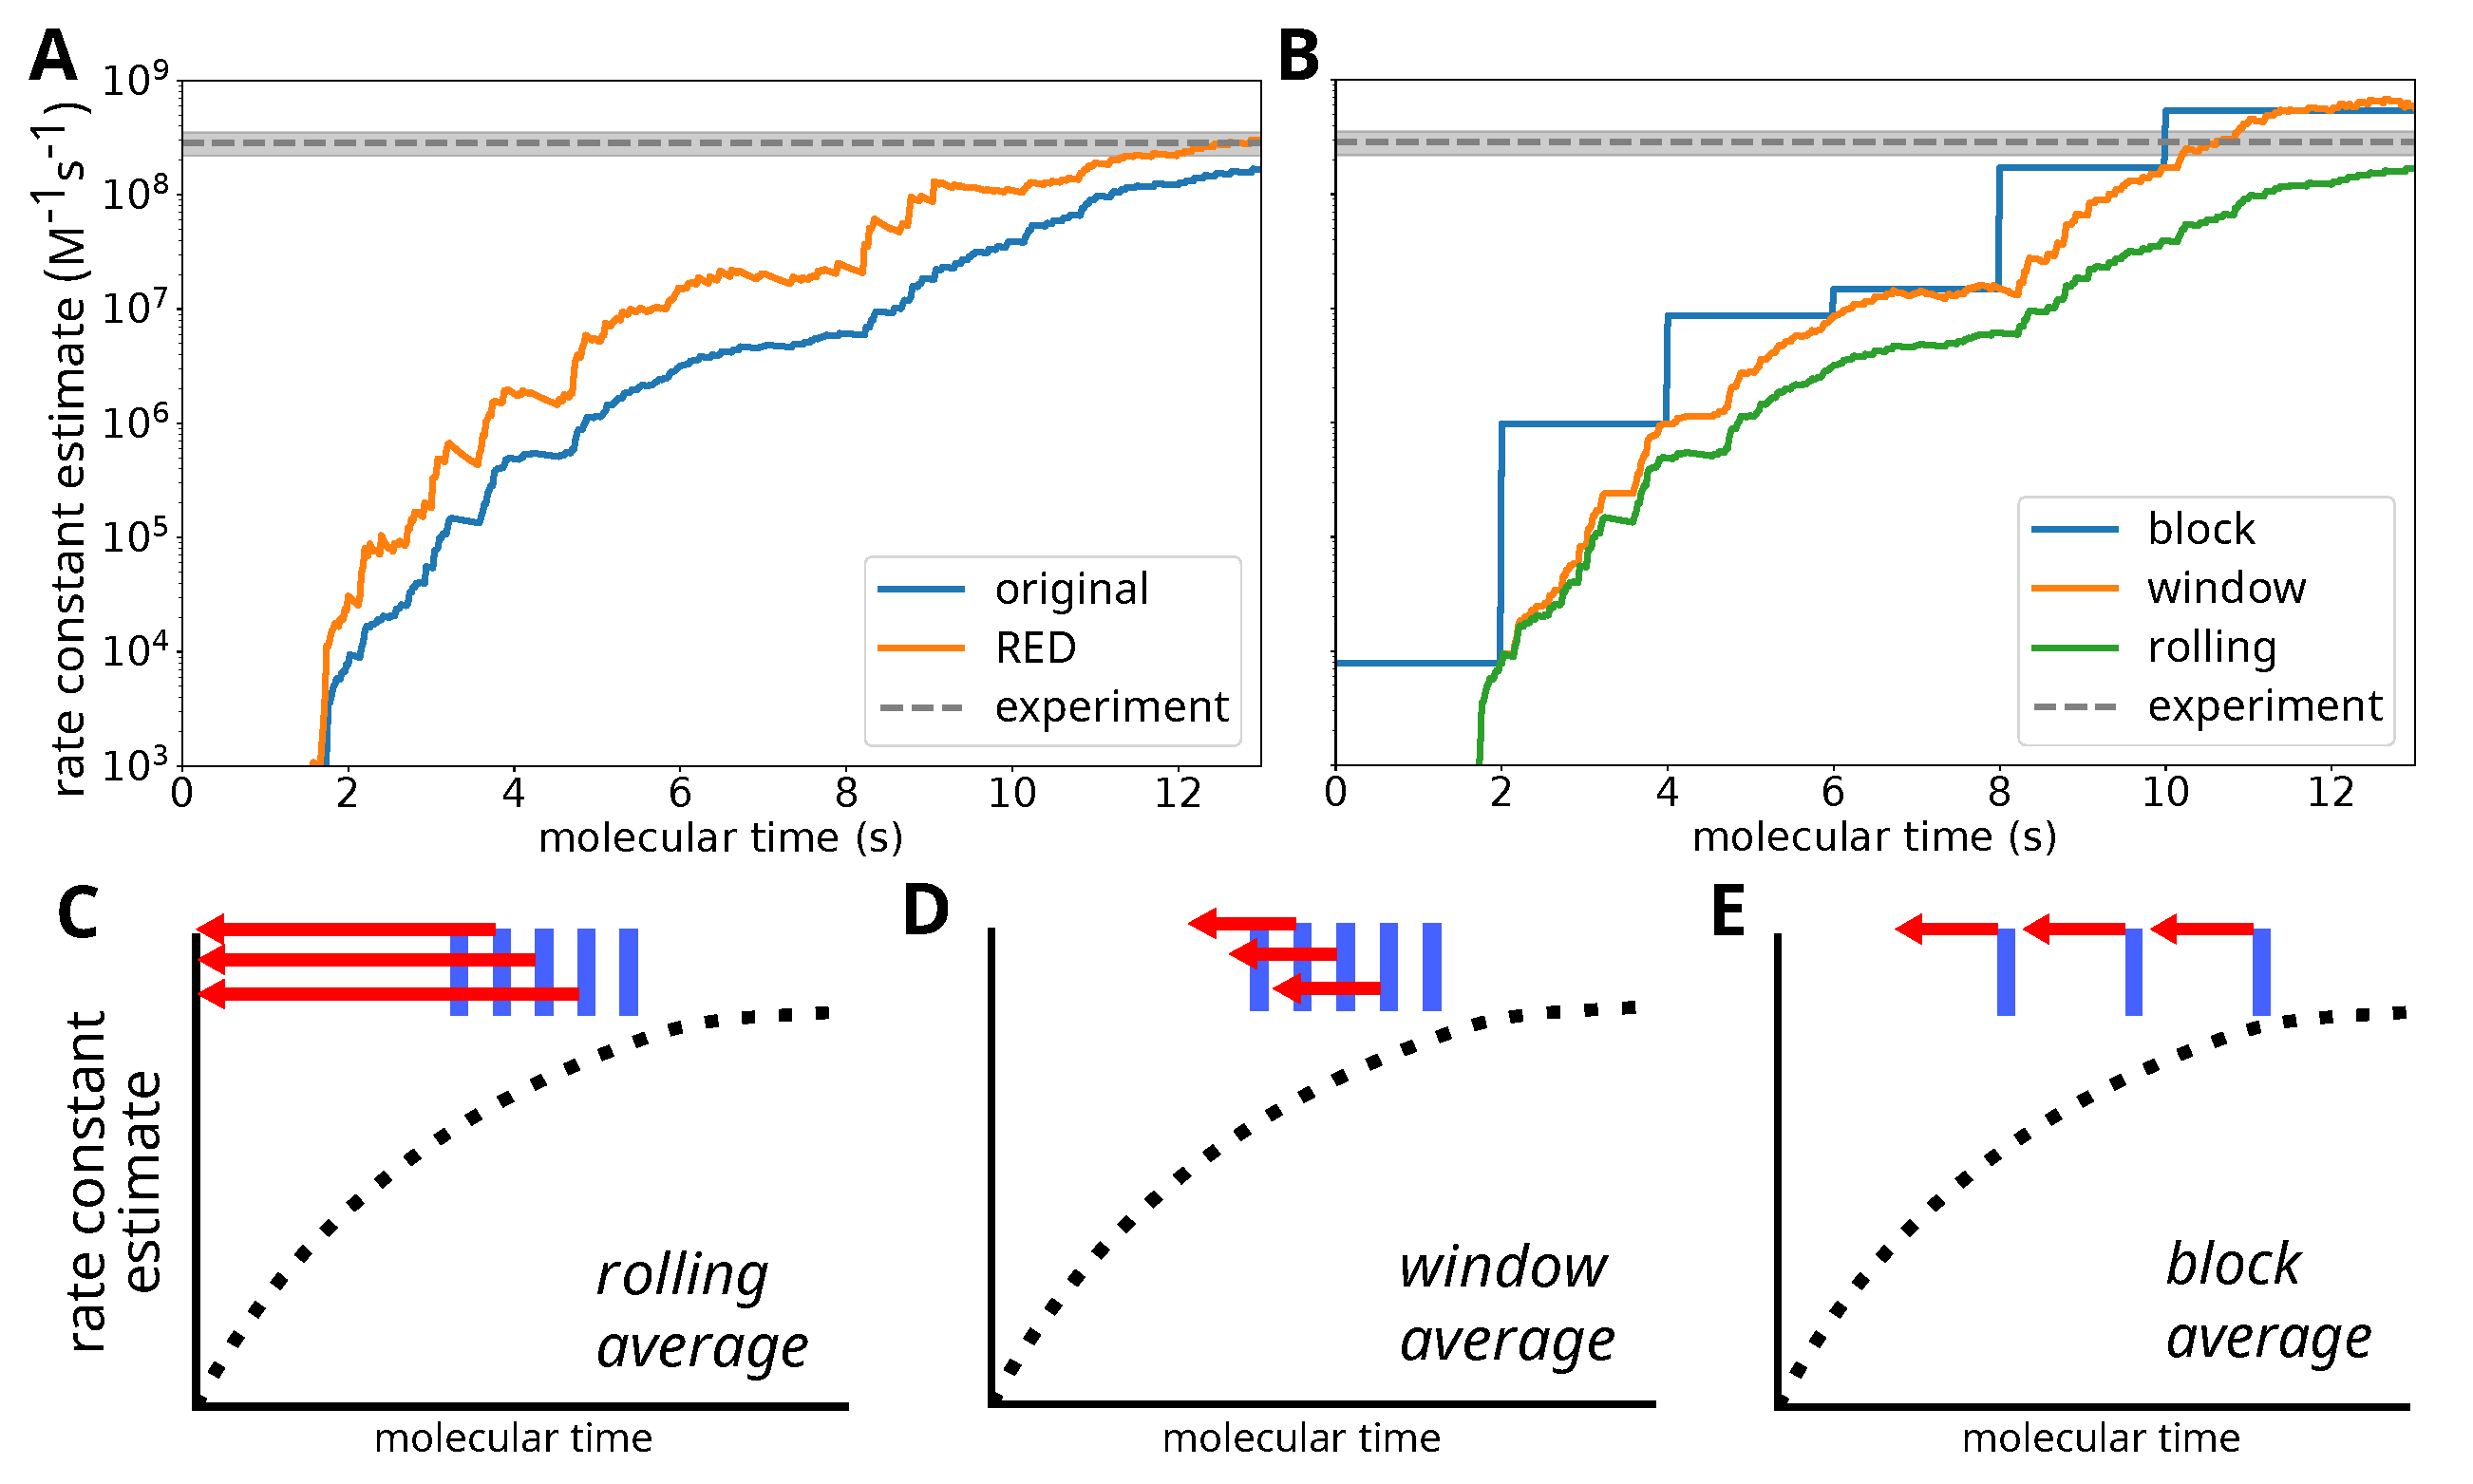
\includegraphics[width=\columnwidth]{figures/Figure8_analysis.pdf}
\vspace{-0.5cm}
\caption{A) A comparison of the RED and original schemes for estimating the rate constant for protein-protein association involving the barnase/barstar system from previously published WE simulations \citep{saglam_proteinprotein_2019}.
In this case, the simulation has not converged to a steady state, as indicated by different rate-constant estimates using the original and RED schemes.
B) A comparison of different averaging schemes using the same dataset.
While the RED scheme is, in principle, only compatible with rolling averages, the use of block and window averaging can still be informative for monitoring convergence of the simulation.
C-E) Schematic illustrations of rolling, window, and block averaging schemes, indicating points where averages are calculated (blue) and the extent of data used for the averages (red).}
\label{fig:red-flux}
\vspace{-0.25cm}
\end{figure}

\pagebreak

\textbf{A note on averaging schemes.} 
There are three main types of averaging schemes that can be used to monitor convergence when plotting the rate constant evolution using the original scheme.
It may be useful to plot different schemes depending on the behavior of your specific system.
A few examples are shown here with instructions on how to generate the plots.

The first averaging scheme is the default which is a rolling average (\textbf{Figure \ref{fig:red-flux}B}), which can be achieved by specifying \verb|evolution: cumulative| in the analysis section of \verb|west.cfg| and setting \verb|step_iter: 1|.
This method of visualizing the rate constant evolution offers the smoothest curve and is recommended as the most stringent way of assessing convergence, as it incorporates information from the entire simulation.
A rolling average is also implicitly incorporated into the RED scheme, which by design never excludes data from the start of a simulation.
When analyzing rate constant estimates generated by the RED scheme, specify \verb|evolution: cumulative| to ensure that only the implicit rolling average is performed.

The second averaging scheme is a window average, which can be achieved in \verb|w_ipa| by specifying \verb|evolution: cumulative| and \verb|step_iter: 10|, or whatever your desired averaging window is.
A recommended starting averaging window size is 10\% of the length of your simulation, but the most robust would be the lag time of your simulation as determined from an autocorrelation of the flux plot.
A windowed average is not as smooth as the rolling average but can give a better indication of convergence at different stages of your simulation relative to other stages.

The third and final averaging scheme is a block average.
This will require setting \verb|evolution: blocked| and \verb|step_iter: 10|.
The rationale behind choosing the block size here is the same as the window size discussed above.
The block average will appear like a step function where each block an average of the preceding block is plotted.
This method of plotting is the least smooth, but can be best for obtaining a final value of the rate constant that is not influenced by earlier, lower values.
\vspace{-0.3cm}

\subsubsection{Conclusion}

Among the upgrades introduced in the WESTPA 2.0 software package are ones that enable the creation and execution of more streamlined analysis of simulations and more efficient estimation of rate constants.
The \verb|westpa.analysis| subpackage can be utilized to more carefully inspect WESTPA trajectory data and to create custom analysis routines.
The RED analysis scheme for correcting rate constants based on the “ramp-up” time in the fluxes is implemented in the \verb|w_red| command-line tool.
The files contained in this tutorial for utilizing the RED scheme are intended to provide useful starting points for analyzing the kinetics of WESTPA simulations.
\pagebreak

\subsection{Advanced Tutorial: M-WEM Simulations of Alanine Dipeptide}
\label{tut:wem-adv}

\subsubsection{Introduction}

The Markovian Weighted Ensemble Milestoning (M-WEM) approach \citep{Ray2022Markovian} is a modified version of the Weighted Ensemble Milestoning (WEM) \citep{Ray2020Kinetics,Ray2020Weighted} approach. 
Both approaches are designed to use the WE strategy to enhance the efficiency of the milestoning method in calculating equilibrium and non-equilibrium properties (e.g., free energy landscape and rate constants, respectively). 

In the milestoning method \citep{Faradjian2004Computing,West2007Extending} the reaction coordinate is stratified using multiple high-dimensional interfaces---or milestones. 
Short trajectories are propagated between the interfaces and using the principles of continuous time Markov chains, the properties of a long timescale process can be calculated. 
But the milestones need to be placed significantly far from each other to lose memory of the previous milestone. 
But converging the transition statistics between distant milestones can be expensive depending on the underlying free energy landscape and the complexity of the system. 
Because of the use of shorter trajectories that do not require trajectories to transit from the initial to final states, the WEM and M-WEM calculations are computationally less expensive than a WE simulation. 
On the downside, however, one cannot obtain continuous pathways due to the lack of continuous trajectories between the starting and the final state. 

In the M-WEM approach, regions between the milestones are referred to as “cells”.
WE simulation is performed within the cell with half-harmonic walls present at the milestone interfaces to prevent trajectory escape \citep{Vanden-Eijnden2009Markovian, Maragliano2009Free, Ray2022Markovian}. 
In this tutorial, we will use M-WEM to calculate the mean first passage time (MFPT), free energy landscape and committor function for the conformational transition in the alanine dipeptide system.

\textbf{Learning objectives.} This tutorial covers the installation of and use of the Markovian Weighted Ensemble Milestoning (M-WEM) software in combination with WESTPA to compute the kinetics and the free energy landscape of an alanine dipeptide. 
Specific learning objectives include:

\begin{enumerate}
  \item How to install the M-WEM software and perform an M-WEM simulation;
  \item How to create milestones to define the M-WEM progress coordinate;
  \item How to analyze an M-WEM simulation to compute the mean first passage time, committor, and free energy landscape. 
\end{enumerate}

\subsubsection{Prerequisites}

The users should have a basic understanding of running WE simulations using the Minimal Adaptive Binning (MAB) scheme, and should have completed \textbf{Advanced Tutorial \ref{tut:mem-perm-adv}} before commencing the M-WEM tutorial. 
Also, a basic idea of the Markovian Milestoning framework is necessary. 
For that purpose, the users should refer to the following manuscripts \cite{Vanden-Eijnden2009Markovian, Maragliano2009Free, Ray2022Markovian}.

\textbf{Computational requirements.} In terms of software, this tutorial requires several Python modules (NumPy, SciPy, and Matplotlib) in addition to the WESTPA 2.0 software and NAMD 2.14 simulation package. 

\noindent Note: M-WEM is implemented using the Colvars module in NAMD. 
Please check out the NAMD tutorial ({\url{http://www.ks.uiuc.edu/Training/Tutorials/namd-index.html}}) and colvars tutorial ({\url{https://colvars.github.io/colvars-refman-namd/colvars-refman-namd.html}}).
 
In terms of computer hardware, this tutorial will require approximately 4 GB of disk space. 
Running the simulation 100 WE iterations for each milestone takes \textasciitilde85 min on an Intel Core i5-8250U CPU @ 1.60GHz processor with 4 CPU cores. 
For 8 milestones that amounts to about 11-12 hr if the calculation is performed serially with 4 CPU cores used at a time. 
But if a computer cluster is available, each milestone should be run in parallel which will significantly reduce the wall clock time. 
The analysis for each milestone takes \textasciitilde5 min for each milestone with the same computing hardware but with 1 CPU core. 
For 8 milestone cells that would be \textasciitilde40 min, but similar to the simulation, the analysis for each milestone can be done in parallel.  

\subsubsection{Installation of the M-WEM software package}

The \verb|M-WEM| software package can be downloaded from {\url{https://github.com/dhimanray/MWEM}}. 
To install the package go to the main directory that contains the \verb|setup.py| file and run the following command:

\begin{verbatim}
  $ python -m pip install .
\end{verbatim}

The M-WEM software should be installed in the same conda environment in which WESTPA 2.0 is installed.

\subsubsection{Setting up a M-WEM environment}

\textbf{Overview.} For performing the M-WEM simulation, we need to first create the milestone anchors along the transition pathway. 
This is a typical prerequisite for milestoning simulation. 
It is typically done using steered MD simulation \citep{griebel_steered_1999} which is a common technique in MD simulation. 
To avoid spending extra time and possible variability in the results, we have generated the milestone anchors and provided them in the anchors directory.

% for single column figure don't include the *
\begin{figure}[t]
\centering
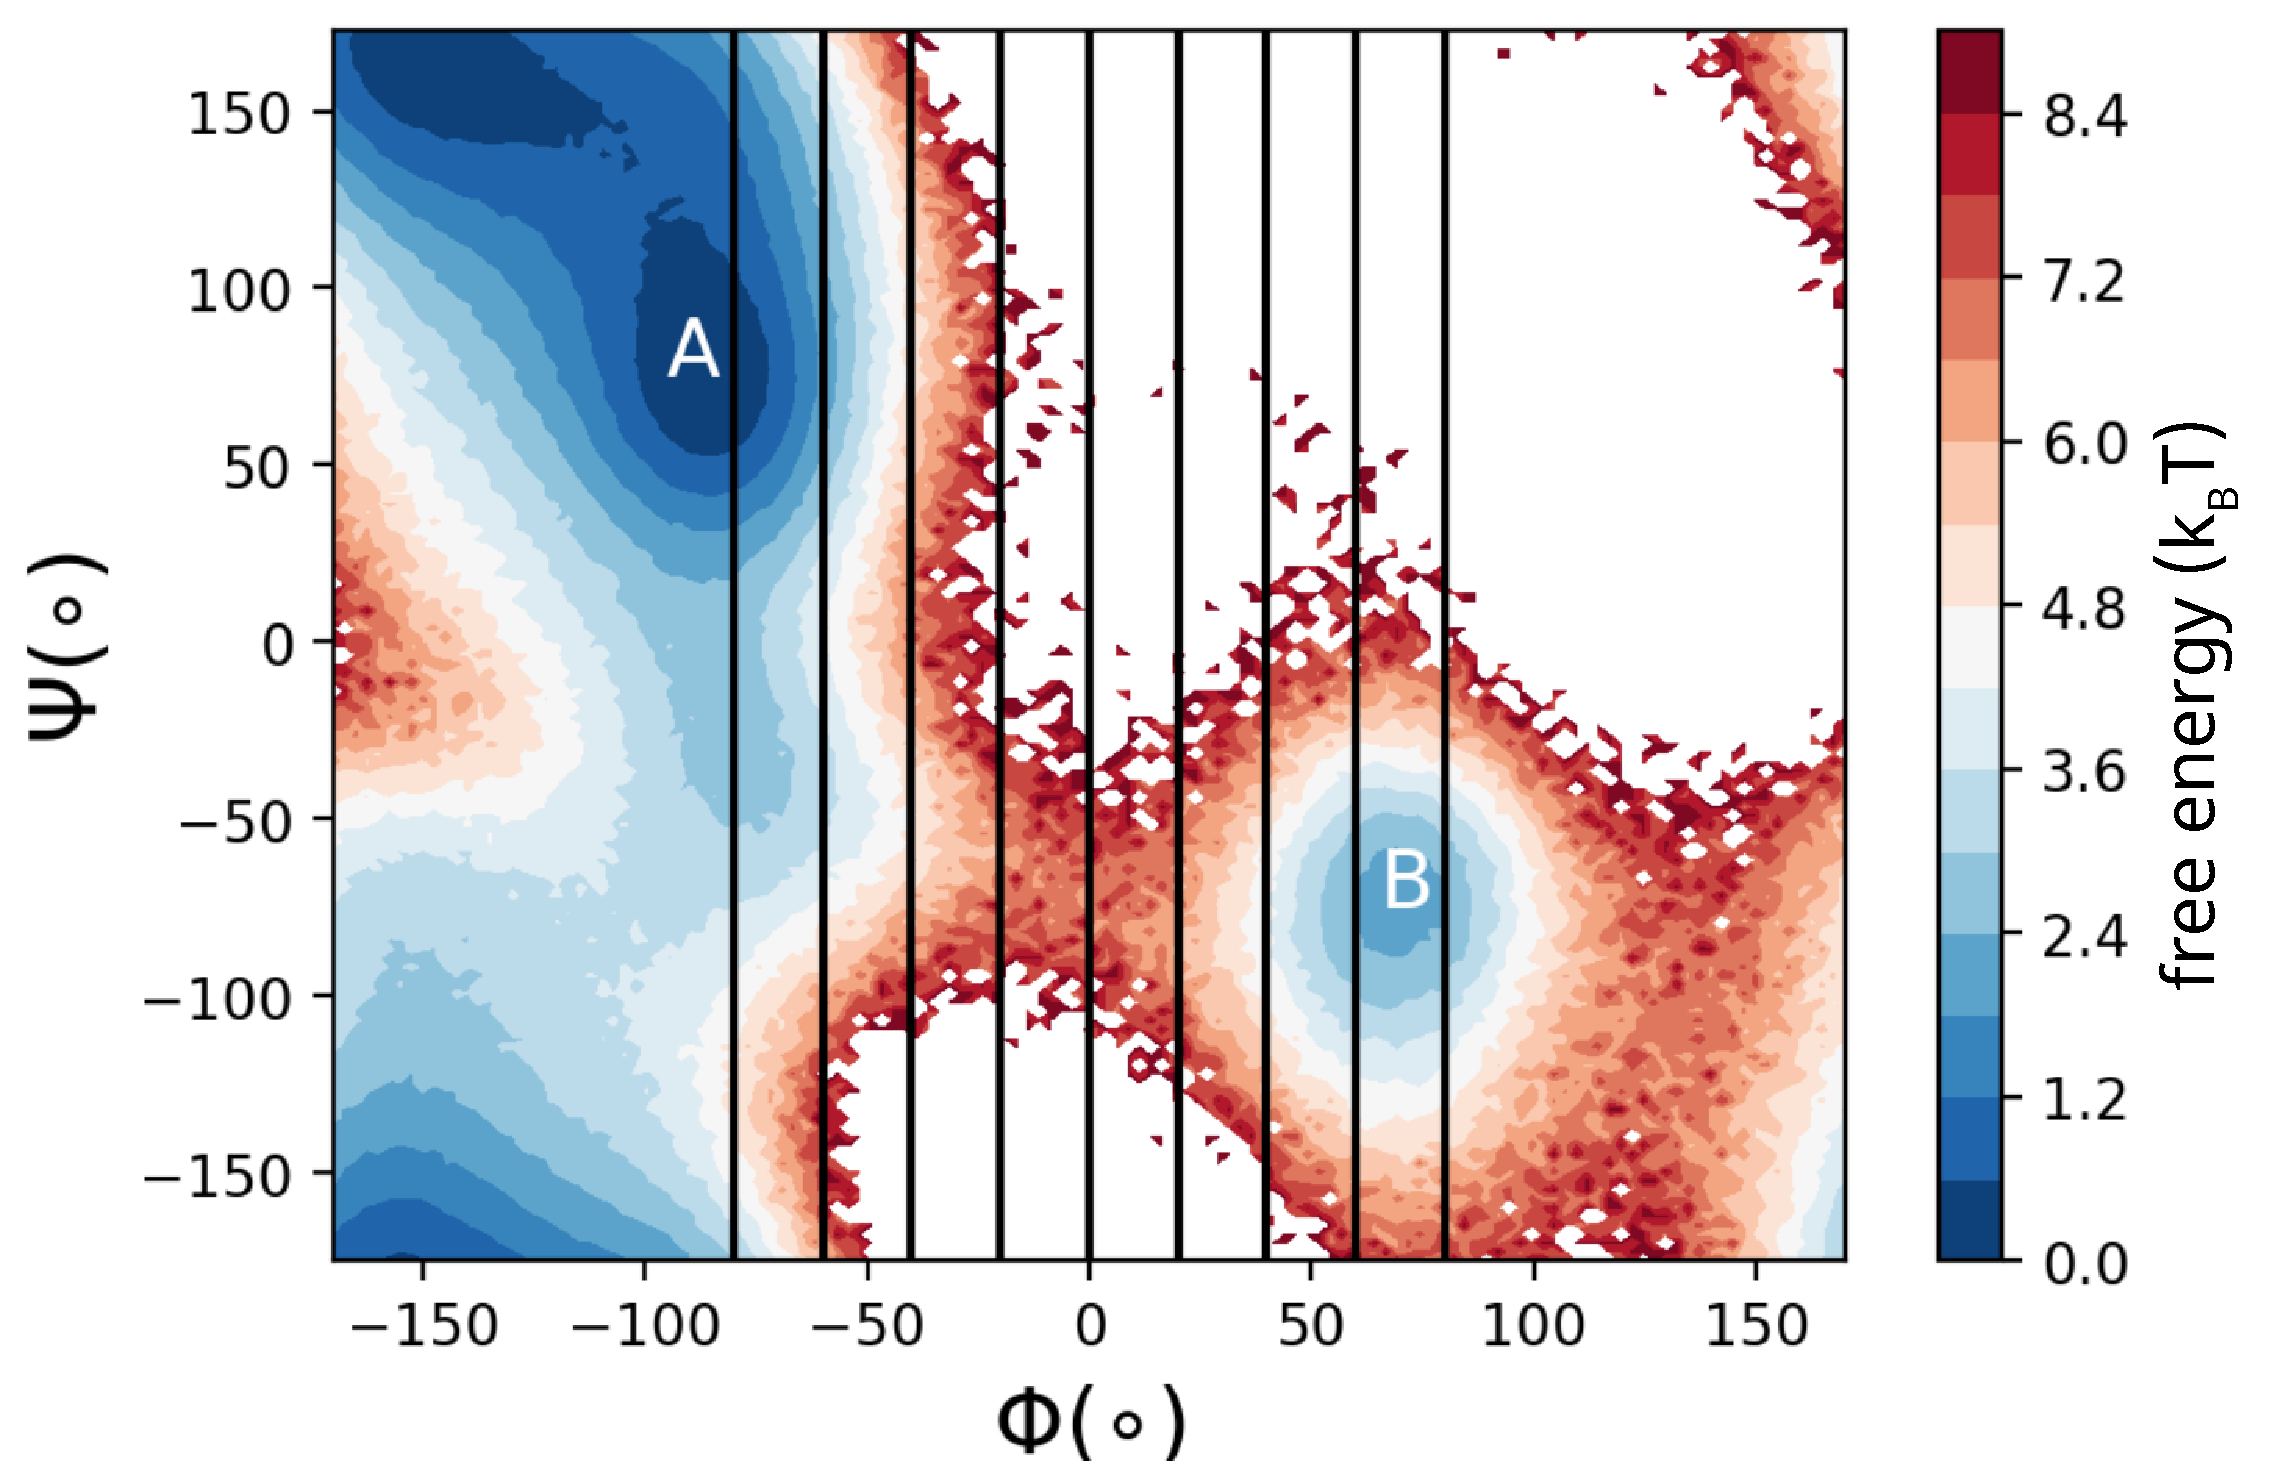
\includegraphics[width=\columnwidth]{figures/Figure9_RBin.pdf}
\caption{Free energy landscape of alanine dipeptide in the gas phase. Milestone positions are shown as vertical lines. 
Our aim is to simulate the MFPT of the transition from state A to state B.}
\label{fig:ala-landscape}
\end{figure}

\textbf{The system.} We will be studying the conformational change of gas phase alanine dipeptide using the M-WEM scheme. 
The details of this example are provided in \citep{Ray2022Markovian}. 

The free energy landscape for the system is shown in \textbf{Figure \ref{fig:ala-landscape}}. 
To simulate the transition from state A to state B, 9 milestones are placed at $\phi$ = -80$^{\circ}$,  -60$^{\circ}$, -40$^{\circ}$, -20$^{\circ}$, 0$^{\circ}$, 20$^{\circ}$, 40$^{\circ}$, 60$^{\circ}$, 80$^{\circ}$. 
This created 8 cells bound by the milestones. 
The anchors are chosen in a way that they are located approximately in the middle of each cell.

\textbf{Preparing the simulation environment.} The \verb|tutorial-7.9/| directory contains all simulation and analysis files and will be referred to as the simulation home directory for the rest of the tutorial. 
The milestone anchors for all cells generated from the steered MD simulation are provided as pdb files in the \verb|anchors/| directory. 

The \verb|build.py| script is a python script which will set up all the milestones for the simulation. 
Each milestone cell will be simulated in a different directory, numbered from 0 to 7. 

The \verb|template/| directory is a generic template for M-WEM simulation for any one cell. 
It contains all necessary files except for the pdb files which are specific to each cell (which are in the \verb|anchors/| directory). 
Also, the \verb|colvars.in| files have replaceable strings which are used by the \verb|build.py| script to create cell specific files. 
For example, there are terms like "CENTER", "HIGH", and "LOW". These are places where the position of the center and the two milestones are written by the \verb|build.py| code. 
Make sure to edit the \verb|env.sh| file to include the path to your NAMD installation.

In the \verb|common_files/| directory the topology (.psf), the parameter (.prm) and the NAMD configuration files are provided. 
The structure file (.pdb) in this directory and in the \verb|equilibration/| directory are prepared by the \verb|build.py| script, and are different for each milestone cell. 

Once you have your M-WEM setup ready, prepare the cell-specific folders by running the following command:

\begin{verbatim}
    $ python build.py
\end{verbatim}

\subsubsection{Running the M-WEM simulation} In the \verb|equilibration/| directory of each cell, a constrained equilibration of the anchor will need to be performed to keep the anchor approximately in the middle of the cell. 
The \verb|milestone_equilibration.colvars.traj| file contains the collective variable information, which, in this case, are the Phi and Psi torsion angles of the alanine dipeptide. 
The \verb|milestone_equilibration.xsc|, \verb|milestone_equilibration.coor| and\linebreak \verb|milestone_equilibration.vel| files are NAMD restart files that will be used to start WE trajectories from the endpoint of the equilibration simulation. 

The running of the M-WEM simulation for each individual cell is done separately, for the convenience of parallelizing it in a computing cluster. 
The \verb|run.sh| script performs the simulation via the command \verb|./run.sh|.
Unlike typical WESTPA setups, the initialization setup code is included in the \verb|run.sh| script here. 
Although it does not make a significant difference for a small system like this, we found it is more convenient to submit multiple milestone jobs to a computer cluster by using a single \verb|run.sh| script. 
Both the equilibration and running of each cell is performed by executing the following command from within each cell-specific folder:

\begin{verbatim}
  $ ./run.sh
\end{verbatim}

In the first part of the script, equilibration is performed. 
Then relevant files are copied to the \verb|bstates/| directory, from which they are read by the \verb|westpa_scripts/runseg.sh|. 
Then the WE simulation is initialized and propagated as usual by the \verb|w_init| and \verb|w_run| commands. 
In this example script, only one trajectory is propagated at a time. 
But this can be parallelized based on the computing resources available.
Alternative Slurm scripts for running and restarting the simulation are also provided in the same directory.

The total number of iterations performed per milestone is 100. 
The user may choose to change this number according to their preference. 
The results reported in this work are from 100 iterations. 
The convergence is achieved after 40 iterations in our calculation. 
But it may slightly vary for independent calculations.

\subsubsection{Analyzing the M-WEM simulations} After the M-WEM simulations are completed, it is important to properly analyze the results. 
Please refer to the M-WEM publication for the theoretical details of the analysis \cite{Ray2022Markovian}. 
We perform the analysis in two steps:

\textbf{Step 1.} Move into the \verb|analysis/| directory and execute the following command: 

\begin{verbatim}
  $ python analysis_build.py 
\end{verbatim}

The \verb|analysis_build.py| script will produce directories \verb|cell_0/| through \verb|cell_7/| and copy the corresponding \verb|west.h5| files (WESTPA output files) from the \verb|propagation/| directory into each cell. 
It will also copy the \verb|west.cfg| files (different from the \verb|west.cfg| files for propagation), and the \verb|analysis.py| files from \verb|westpa_analysis_files/| directory to each cell. 
The \verb|analysis.py| file also has strings like "LOW" and "HIGH", which will be replaced by floating point numbers corresponding to the left and right milestones.

Running the \verb|analysis.py| script from within a specific cell directory will produce the \verb|trajectories.pkl|, \verb|crossings.pkl| and \verb|weights.txt| files. 
The files generated by \verb|analysis.py| contain information on the trajectory traces (history of the segments in the final iteration), the time and location (which milestone right or left) of the milestone crossings, and the weights of each traced trajectory respectively.


% for single column figure don't include the *
\begin{figure}[t]
\centering
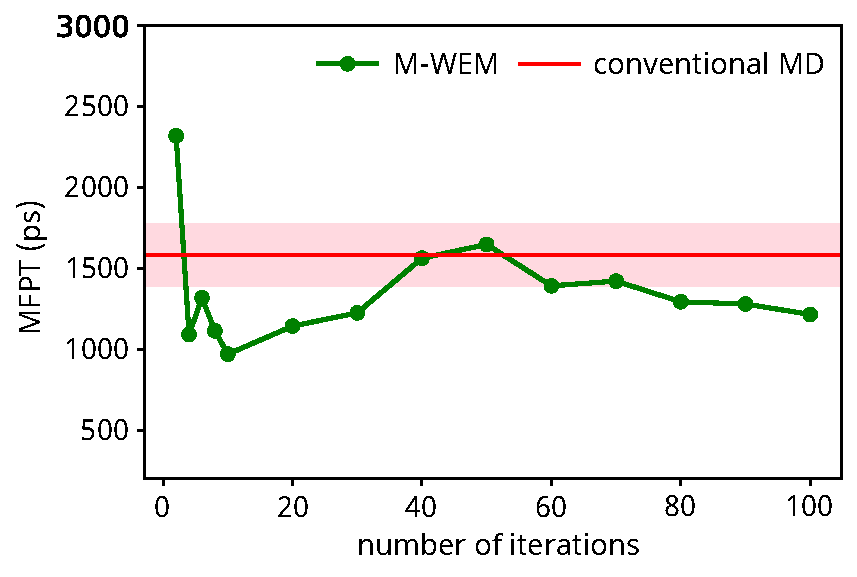
\includegraphics[width=\columnwidth]{figures/Figure10_MFPT.pdf}
\caption{Convergence of the mean first passage time (MFPT) as a function of M-WEM iterations.}
\label{fig:mwem-mfpt}
\end{figure}

Perform analysis in all cells by running the following command from within the \verb|analysis/| directory:

\begin{verbatim}
  $ ./analyze_all_convergence.sh
\end{verbatim}

This script will execute \verb|python analysis.py| from within each cell-specific directory to produce the .pkl and .txt outputs for the final iteration. 
But, for the sake of checking convergence of our results, it will also produce similar files for some subsequent iterations. 
To do that, the script will copy the \verb|analysis.py| to \verb|analysis_x.py| (where x = iteration number) and replace the \verb|w.niters| inside each \verb|analysis.py| to the corresponding iteration number. 
Then, it will produce \verb|trajectories_x.pkl|, \verb|crossings_x.pkl| and the \verb|weights_x.txt| files for each x. 
This step can take several minutes to a few hours depending on the computing hardware. 
If you have access to a computing cluster, you may choose to submit this as a job.
Note that the \verb|analyze_all_convergence.sh| script is customizable. 
For example, if you want to run all cells in parallel on a cluster you can create separate bash scripts for each cell. 
Also, \verb|analysis_build.py| will produce the following directories for milestoning analysis in Step 2: \verb|cell_probability/|, \verb|N_i_j_files/|, \verb|R_i_files/|, and \verb|committor/|.

% for single column figure don't include the *
\begin{figure}[t]
\centering
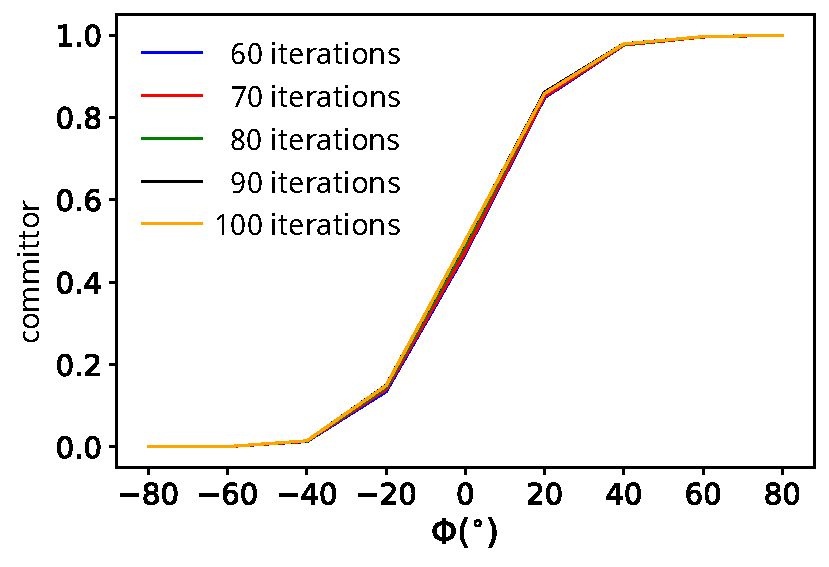
\includegraphics[width=\columnwidth]{figures/Figure11_Committor.pdf}
\caption{Committor function along the $\phi$ coordinate from M-WEM simulation.}
\label{fig:mwem-committor}
\end{figure}

\textbf{Step 2.} After the analysis of the WESTPA output files are done, we will proceed to analyze our results using the Markovian milestoning framework in two Jupyter notebooks: \verb|kinetics.ipynb| and \verb|free-energy-landscape.ipynb|.

First, run the \verb|kinetics.ipynb| notebook to obtain the mean first passage time and the committors. 
This will also produce the probability distribution file in the milestone space. Details can be found inside the notebook. 
The MFPT convergence plots and the committor functions should look like \textbf{Figures \ref{fig:mwem-mfpt} and \ref{fig:mwem-committor}}.

Next, run the \verb|free-energy-landscape.ipynb| to reconstruct the free energy landscape along Phi and Psi coordinates from the M-WEM data. 
It will first produce the unscaled probability distribution, rescale it and then compute the rescaled free energy landscape. 
The final free energy landscape should look like \textbf{Figure \ref{fig:mwem-landscape}}.

Note that before executing any notebook, you will need to set the kernel to the environment in which you installed the M-WEM software. 
If the kernel is not available, activate the Jupyter notebook for that environment by executing:

\begin{verbatim}
  $ python -m ipykernel install --user --name=westpa2
\end{verbatim}
Replace \verb|westpa2| with the environment in which you installed M-WEM.

% for single column figure don't include the *
\begin{figure}[t]
\centering
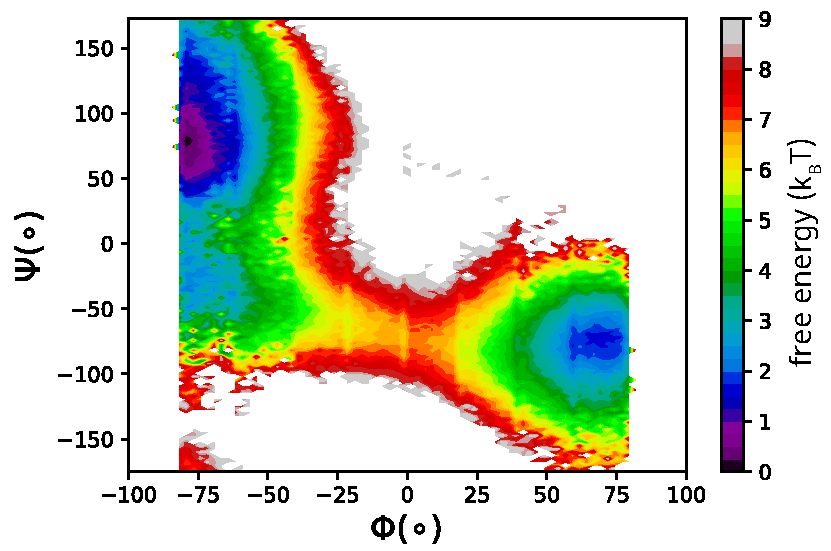
\includegraphics[width=\columnwidth]{figures/Figure12_RFree.pdf}
\caption{Free energy landscape reconstructed from an M-WEM simulation.}
\label{fig:mwem-landscape}
\end{figure}

\subsubsection{Conclusion}
This tutorial presents the Markovian Weighted Ensemble Milestoning (M-WEM) Python package for use with the WESTPA 2.0 software package to estimate equilibrium and non-equilibrium observables for the alanine dipeptide. 
In the M-WEM approach, the WE strategy is applied to enhance the efficiency of the Markovian milestoning approach to accelerate the convergence between milestones.
While it is not possible to use this approach to generate continuous pathways between the initial and final states of a rare-event process, the M-WEM approach can be highly efficient in the calculation of  “end-point properties” such as the MFPT and free energy differences between the two states. 
Beyond the alanine dipeptide, the M-WEM approach has been applied to more complex processes such as receptor-ligand binding, yielding the $k_{on}$, $k_{off}$, and binding free energy for the trypsin benzamidine complex \citep{Ray2022Markovian}.

\subsection{Advanced Tutorial: Systems Biology Simulations using the WESTPA/BNG Plugin}
\label{tut:bng-adv}

\subsubsection{Introduction}
This tutorial focuses on a scenario in systems biology in which the WE strategy can be useful: enhanced sampling of rare events in a non-spatial model. 
Here we focus on a BioNetGen language (BNGL) rule-based model for a biological signaling network that consists of a set of structured molecule types and a set of rules that define the interactions between the molecule types. 
While the average steady-state behavior of the model can be obtained using ordinary differential equations, the full kinetics of the model can only be obtained from stochastic simulations. 
However, adequate sampling of any rare events in the model can be a challenge for stochastic simulations. 
In this tutorial, we will use WESTPA to orchestrate BNGL simulations that are propagated by the BNG software package. 
As mentioned above, WESTPA is interoperable with any stochastic dynamics engine, including the BNG software.

\pagebreak

\textbf{Learning objectives.} We will simulate a BNGL rule-based model of a two-gene switch motif that exhibits mutually exclusive activation and inhibition.
Specific learning objectives include:
\begin{enumerate}
    \item How to install the WESTPA/BNG plugin and set up a WESTPA/BNG simulation; 
    \item How to apply adaptive Voronoi binning, which can be used for both non-spatial and molecular systems; 
    \item How to run basic analyses tailored for high-dimensional WESTPA/BNG simulations.
\end{enumerate} 

\subsubsection{Prerequisites}
Users should have a working knowledge of BNGL models ({\url{http://bionetgen.org}}) and the WESTPA 2.0 software package. 
This tutorial will make use of the WEBNG Python package, which facilitates the integration of WESTPA with the BNG software and requires Python 3.8 or later versions. 
To install the WEBNG package: 

\begin{verbatim}
  $ git clone 
        https://github.com/ASinanSaglam/webng.git
  $ python -m pip install -e .
\end{verbatim}

For common installation issues, see {\url{https://webng.readthedocs.io/en/latest/quickstart.html#installation}}. Alternatively the user can use a Docker container where the environment is already prepared correctly using the command: 
\begin{verbatim}
  $ docker pull 
          ghcr.io/westpa/westpa2_tutorials:webng
\end{verbatim}

Note that this requires a Docker installation, for more information see Docker documentation ({\url{https://docs.docker.com/get-docker}}). 
Once the docker image is downloaded, you can run the image with:
\begin{verbatim}
  $ docker run -it --entrypoint /bin/bash 
            ghcr.io/westpa/westpa2_tutorials:webng
\end{verbatim}

\textbf{Computational requirements.} This tutorial requires \textasciitilde500 MB disk space. 
The simulation takes at most 1 hour of wall-clock time using a single CPU core of a 3.2GHz Intel Core i7 processor. 
We recommend using the \verb|WEBNG| package on a Unix system. 
While the package has not been tested on Windows systems, one can try using the Windows subsystem for Linux (WSL; {\url{https://docs.microsoft.com/en-us/windows/wsl/install}}).

\subsubsection{Setting up the simulation}

\noindent\textbf{The model.} Our BNGL model consists of two genes, gene A and gene B, that are transcribed to produce proteins A and B, respectively (\textbf{Figure \ref{fig:two-gene-model}}). 
Protein A binds to the gene A promoter site to activate protein A production and to the gene B promoter site to repress B production. 
Likewise, protein B activates gene B and represses gene A. 
The two most populated states therefore consist of either (1) high quantities of protein A and low quantities of protein B, or (2) high quantities of protein B and low quantities of protein A. 
Transitions between these two states are rare events. 

\begin{figure}[t]
\centering
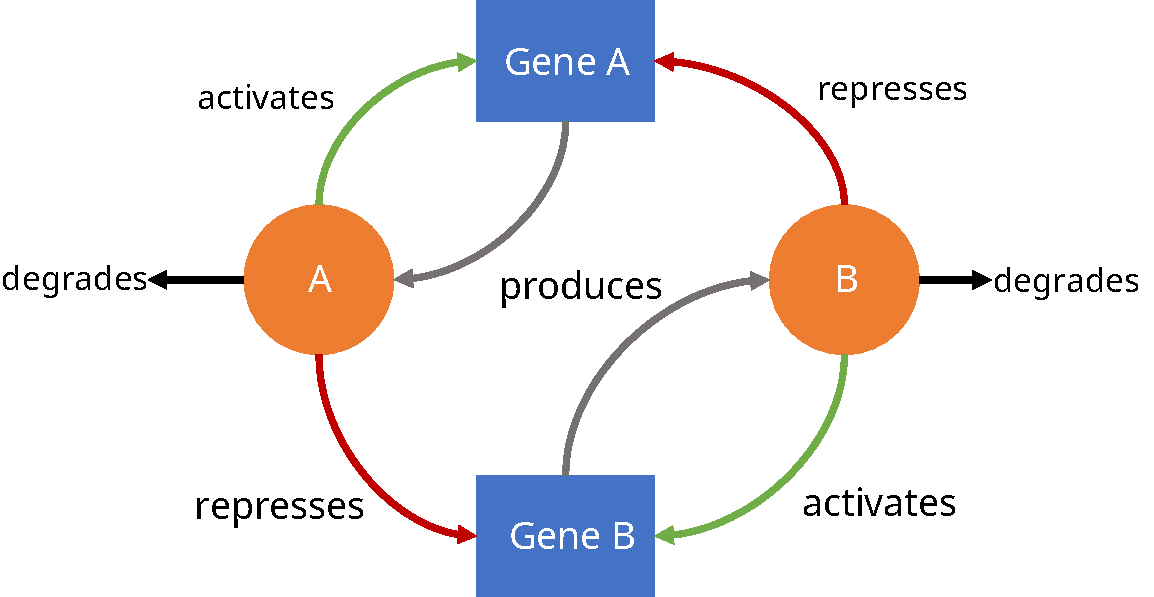
\includegraphics[width=\columnwidth]{figures/Figure13_Network.pdf}
\caption{Two-gene network of exclusive mutual inhibition and self activation.  Blue squares represent genes and orange circles represent proteins.}
\label{fig:two-gene-model}
\end{figure}

\textbf{Preparing the simulation environment.} For this portion of the tutorial, you can use either your own BNGL model or the ExMISA model described above, which is the default WEBNG example. 
WEBNG uses a YAML configuration file to set up a WESTPA folder. 
The \verb|WEBNG template| subcommand gives you a YAML config file with the same defaults which you can then edit and use to generate the WESTPA simulation folder. 

If you are using the default example, the command to generate the template is the following:
\begin{verbatim}
  $ webng template -o mysim.yaml 
\end{verbatim}

If you are using your own model file called \verb|exmisa.bngl|, the command is:
\begin{verbatim}
  $ webng template -i exmisa.bngl -o mysim.yaml
\end{verbatim}

This command will generate the YAML file, \verb|mysim.yaml|. For the full set of configuration options, see {\url{https://webng.readthedocs.io/en/latest/config.html}}. 
Path options are specified automatically using the libraries that are already installed. 
Propagator options will also be automatically populated according to the BNGL model. 
By default, this simulation setup will use an adaptive Voronoi binning scheme \citep{zhang_exact_2010} due to the fact that rectilinear binning is not feasible for high-dimensional BNG models. 
The \verb|center_freq| option sets the frequency of Voronoi bin addition, in units of WE iterations, \verb|max_centers| is the maximum number of Voronoi bins that will be added, \verb|traj_per_bin| is the number of trajectory walkers per Voronoi bin, and \verb|max_iter| option sets the maximum number of WE iterations. 
All of these options can be modified after the simulation folder is set up (see {\url{https://github.com/westpa/westpa/wiki/User-Guide#Setting_Up_a_WESTPA_Simulation}}). 

By default, the stochastic simulator is set to libroadrunner ({\url{http://libroadrunner.org}}). 
To use this simulator, we must first convert the BNGL model to a systems biology markup language (SBML) model. 
Next, we use the WEBNG software to compile the SBML model into a Python object, which allows for efficient simulation of the model. 
WEBNG also supports the use of the \verb|BNG| simulation package. 
However, the use of this package will result in higher file I/O operations. 
Any other stochastic simulator will require the use of a custom WESTPA propagator.

\subsubsection{Running the WE simulation}
To run the simulation, we first need to generate a WESTPA folder using the YAML configuration file generated in the previous step:

\begin{verbatim}
  $ webng setup --opts mysim.yaml
\end{verbatim}

The above command will use the path option \verb|sim_name| as the WESTPA folder, which is automatically set to the model name in the folder you ran the template command. 
Next, we initialize the simulation and run the model in a serial mode using a single CPU: 

\begin{verbatim}
  $ cd exmisa
  $ ./init.sh
  $ w_run --serial
\end{verbatim}

To run the model in a parallel mode using multiple CPU cores, please refer to WESTPA documentation for options available with the \verb|w_run| command-line tool.
The resulting simulation can be found in the \verb|exmisa/| folder directory.

\begin{figure}[t]
\centering
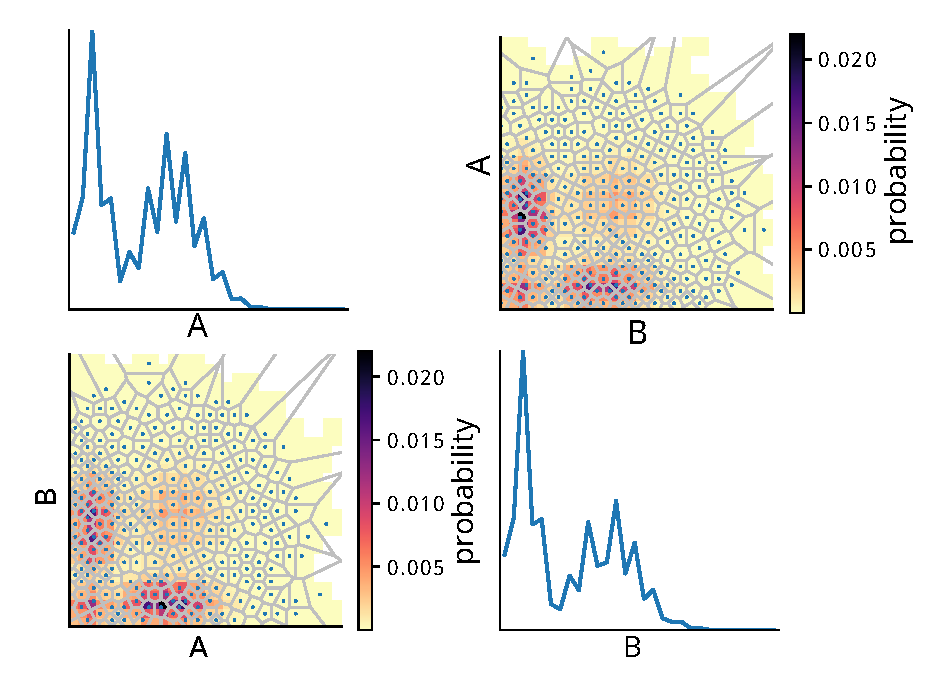
\includegraphics[width=\columnwidth]{figures/Figure14_ProbDist.pdf}
\caption{Probability distributions as a function of the two-dimensional progress coordinate (off-diagonal) and each dimension of the progress coordinate (diagonal).
Axes A and B show the quantity of each protein in the two-gene model.
Grey lines in each off-diagonal plot delineate adaptive Voronoi bins used during the WE simulation.}
\label{fig:bngl-bins-proteins}
\end{figure}

\begin{figure}[t]
\centering
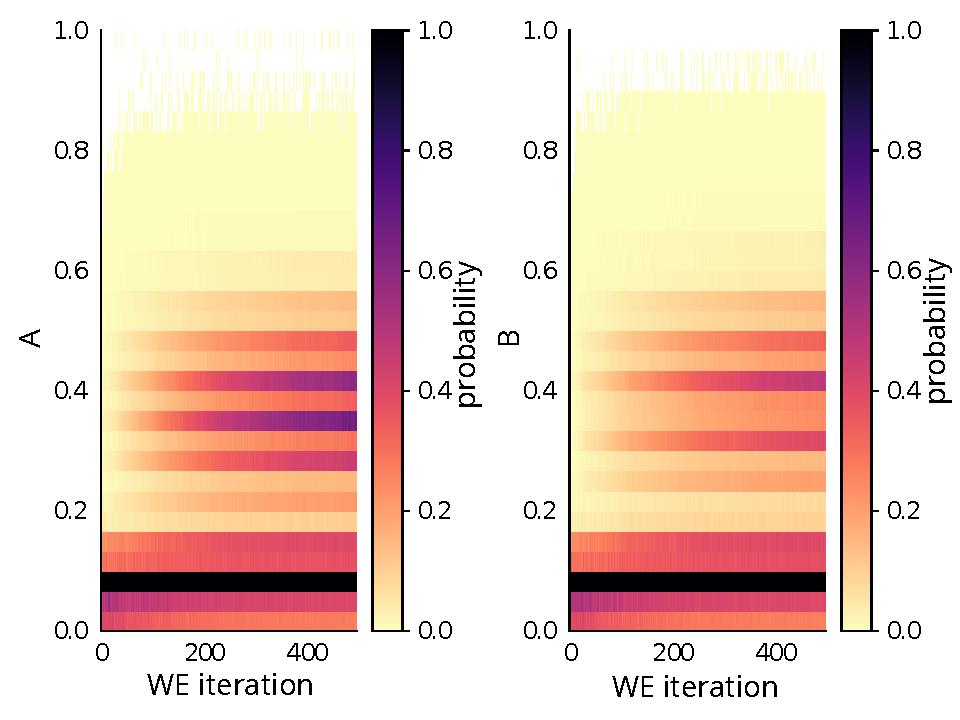
\includegraphics[width=\columnwidth]{figures/Figure15_ProbDist2.pdf}
\caption{Probability distributions of each observable (A or B) of the two-dimensional progress coordinate as a function of WE iteration. 
The striped nature of the distributions is due to the fact that A and B are discrete as opposed to continuous observables.}
\label{fig:bngl-iterations}
\end{figure}

\subsubsection{Analyzing the WE simulation}
To analyze the simulation, we will use the WEBNG package. 
To begin, we edit the YAML file under the folder that contains the configuration file \verb|mysim.yaml|, setting \verb|analyses.enable|, \verb|analyses.average.enable|, and \verb|analyses.evolution.enable| to \verb|True|; and \verb|analyses.average.first-iter| to the simulation half point (default: 50). 
To run the analysis, we use the following command: 

\begin{verbatim}
  $ webng analysis --opts mysim.yaml
\end{verbatim}

The above command will generate an \verb|analysis/| folder in the simulation folder, run the analyses, and generate associated figures. 

By default, \verb|average.png| provides an N$\times$N matrix of plots of the average two-dimensional probability distributions of each observable (dimension) of the WE progress coordinate  (\textbf{Figure \ref{fig:bngl-bins-proteins}}) and each of the other observables. 
The \verb|evolution.png| file gives the time-evolution (number of WE iterations) of probability distributions for each observable  (\textbf{Figure \ref{fig:bngl-iterations}}) and can be used to assess the convergence of simulation, making modifications to the binning scheme if necessary. 


The average two-dimensional probability distributions reveal a total of four states: a low A/low B state, the symmetric low A/high B state and high A/low B states, and a high A/high B state  (\textbf{Figure \ref{fig:bngl-bins-proteins}}). 
The fourth state is the least probable while the first three states are all highly probable. 
Transitions from low A/high B to high A/low B states are difficult to sample and transitions from low A/high B to high A/high B states are even more difficult to sample. 
The WE algorithm allows the user to sample these states and transitions between the states. 
All analyses should be based on the portion of the simulation that is done evolving. 
If the simulation is still evolving, we recommend extending the simulation until the observables of interest are reasonably converged. 

\subsubsection{Conclusion}

As demonstrated by this tutorial, the WEBNG Python package provides a framework for applying the WESTPA 2.0 software package to BNGL models with minimal user input and simplified installation. 
The adaptive Voronoi binning scheme enables efficient application of high-dimensional progress coordinates for both molecular and non-spatial systems.
Voronoi bins can be effective for exploratory simulations, placing bins as far away as possible from previous bins to inform the creation of a custom binning scheme for sampling the rare-event process of interest. 
However, such bins may not be as effective for surmounting barriers (e.g., compared to the MAB scheme \citep{torrillo_minimal_2021}), as demonstrated by the probability distribution as a function of the WE progress coordinate where many bins near the edges of the configurational space are occupied, but are not of interest. 
Future work with WEBNG will include more detailed analysis options such as automated clustering, generation of networks from bins and clusters, and the estimation of rate constants for transitions between the clusters. 


\section{Author Contributions}
%\hl{Lllian, please check
%OLD:
%AT Bogetti, B Mostofian, A Dickson, AJ Pratt, AS Saglam, PO Harrison, JL Adelman, M Dudek, PA Torrillo, AJ DeGrave, and U Adhikari developed and wrote the tutorials; the primary author of each tutorial is designated as a co-first author of the overall manuscript and listed in the order in which the tutorials appear in the manuscript. LT Chong and DM Zuckerman provided guidance for tutorial development. 
%AT Bogetti, LT Chong, DM Zuckerman, AJ Pratt, AS Saglam, B Mostofian, and MC Zwier wrote the introductory sections leading up to the tutorials. 

%NEW:
AT Bogetti, JMG Leung, JD Russo, S Zhang, JP Thompson, AS Saglam, and D Ray developed and wrote the Advanced tutorials; the primary author of each tutorial is designated as a co-first author of the overall manuscript. AT Bogetti, B Mostofian, AJ Pratt, AS Saglam, PO Harrison, JL Adelman, M Dudek, PA Torrillo, AJ DeGrave, and U Adhikari developed and wrote the Basic and Intermediate Tutorials \ref{tut:nacl-basic}-\ref{tut:analysis-adv} \citep{bogetti_suite_2019}.
LT Chong, DM Zuckerman, DN LeBard, MC Zwier, JL Adelman, I Andricioaei, and JR Faeder provided guidance for tutorial development. 
AT Bogetti, JMG Leung, LT Chong, DM Zuckerman, and MC Zwier wrote the introductory sections leading up to the tutorials. 
RC Abraham helped generate trajectory data for \textbf{Advanced Tutorial \ref{tut:binless}}.

\section{Other Contributions}
We thank the many users of the WESTPA software who have provided important feedback for improving our tutorials and documentation over the years.  

\section{Potentially Conflicting Interests}
The authors declare the following competing financial interest(s): L.T.C. is a current member of the Scientific Advisory Board of OpenEye Scientific and an Open Science Fellow with Roivant Sciences. S Zhang, JP Thompson, and DN LeBard are employees of OpenEye Scientific.

\section{Funding Information}
This work was supported by NIH R01 GM1151805-01 to LT Chong, DM Zuckerman, and JR Faeder; NSF grants CHE-1807301 and MCB-2112871 to LT Chong; a University of Pittsburgh Andrew Mellon Predoctoral Fellowship to AT Bogetti; and a MolSSI Software Fellowship to JD Russo. 


\section{Content and Links}
%OLD
%All files needed for the tutorials can be found at \url{https://github.com/westpa/westpa_tutorials}

%NEW

All files needed for the tutorials can be found at \url{https://github.com/westpa/tutorials}. 

\section*{Author Information}
\makeorcid

%\bibliography{TutorialsManuscript.bib,15_references.bib}
\bibliography{combo_refs.bib}

\input{stuff_at_the_end_ofV1}
%%%%%%%%%%%%%%%%%%%%%%%%%%%%%%%%%%%%%%%%%%%%%%%%%%%%%%%%%%%%
%%% APPENDICES
%%%%%%%%%%%%%%%%%%%%%%%%%%%%%%%%%%%%%%%%%%%%%%%%%%%%%%%%%%%%

%\appendix


\end{document}
